\documentclass[12pt, a4paper]{report}
\usepackage[margin=1in]{geometry}
\usepackage{graphicx}
\usepackage{hyperref}
\usepackage{setspace}
\usepackage{fancyhdr}
\usepackage{xcolor}
\usepackage{booktabs}
\usepackage{array}
\usepackage{float}

% Set line spacing
\onehalfspacing

% Header and Footer
\pagestyle{fancy}
\fancyhf{}
\rhead{Financial Analysis Report}
\lhead{Indian FMCG Sector}
\cfoot{\thepage}

% Title Page
\title{\textbf{FAA :- Financial Analysis Report} \\ \vspace{0.5cm} \Large Indian Fast Moving Consumer Goods Circuit}
\author{
    \textbf{Team Members:} \\
    \vspace{0.3cm}
    Prabir Kalwani (N069) \\
    Aayush Shah (N087) \\
    Snehil Sinha (N095) \\
    Parampara Srivastava (N101) \\
    Rishabh Mishra (N065) \\
    \vspace{0.8cm}
    \textbf{Faculty Mentor:} \\
    Dr. Geeta Shetty
}
\date{October 2025}

\begin{document}

\maketitle

\newpage
\tableofcontents
\newpage

% ===============================================
% CHAPTER 1: INTRODUCTION
% ===============================================
\chapter{Introduction to the Project}

This report presents a comprehensive financial analysis of key players in the Indian Fast-Moving Consumer Goods (FMCG) sector. The Indian FMCG market represents one of the largest and fastest-growing consumer markets globally, with companies ranging from traditional manufacturing to diversified conglomerates.

The analysis encompasses six major companies: Hindustan Unilever (HUL), Godrej Consumer Products Limited (GCPL), Britannia Industries, Dabur India Limited, Tata Consumer Products Limited, and ITC Limited. These organizations represent diverse segments within the FMCG landscape, including soaps and personal care, food and beverages, healthcare, and household products.

This report examines key financial metrics, corporate governance structures, dividend policies, and strategic positioning of these market leaders in the Indian FMCG circuit.

\section{Purpose and Context}

The Indian Fast-Moving Consumer Goods (FMCG) sector represents one of the country's most dynamic and competitive industries, characterized by high-volume sales, rapid inventory turnover, and intense brand competition. As economic conditions evolve and consumer preferences shift, understanding the financial health and strategic positioning of leading players becomes critical for investors, analysts, and industry stakeholders.

This comprehensive report analyzes the financial performance of six major FMCG companies---ITC Limited, Hindustan Unilever Limited (HUL), Tata Consumer Products, Dabur India, Britannia Industries, and Godrej Consumer Products Limited (GCPL)---comparing their fiscal year 2023 performance against fiscal year 2024 results. These companies collectively represent diverse product portfolios spanning personal care, food and beverages, home care, and tobacco products, providing a holistic view of sector dynamics.

\section{Analytical Framework}

The analysis employs a multi-dimensional financial assessment framework examining four critical areas:

\begin{itemize}
    \item \textbf{Liquidity Analysis} evaluates each company's ability to meet short-term obligations through current and quick ratios, revealing financial flexibility and working capital management effectiveness.
    
    \item \textbf{Profitability Analysis} assesses operational efficiency and pricing power by examining gross and net profit margins, indicating how effectively companies convert revenue into bottom-line earnings.
    
    \item \textbf{Leverage Analysis} examines capital structure through debt-to-equity ratios, revealing financial risk profiles and management's approach to funding growth and operations.
    
    \item \textbf{Operational Efficiency} measures inventory turnover rates, providing insights into supply chain effectiveness, demand forecasting accuracy, and working capital optimization.
\end{itemize}

\section{Market Environment and Relevance}

The FY2023-24 period presented unique challenges for FMCG companies, including persistent inflation in key raw materials, evolving consumer behaviors post-pandemic, increasing rural market pressures, and intensifying competition from both established players and emerging direct-to-consumer brands. Understanding how different companies navigated these headwinds through their financial strategies provides valuable insights into management quality, competitive positioning, and future prospects.

This report moves beyond surface-level ratio comparisons to provide interpretive analysis---exploring the ``why'' behind numerical changes, identifying strategic patterns, and offering actionable insights. By examining year-over-year trends across multiple financial dimensions simultaneously, we uncover interconnected dynamics that reveal each company's true financial health and strategic direction.

\newpage


% ===============================================
% CHAPTER 2: COMPANY PROFILES
% ===============================================
\chapter{Company Profiles: Key Details}

\section{Hindustan Unilever (HUL)}

\subsection{Corporate Information}

\begin{tabular}{ll}
    \textbf{NIC Code} & 20231 (Soap manufacturing and related FMCG) \\
    \textbf{Headquarters} & Unilever House, B. D. Sawant Marg, \\
                          & Chakala, Andheri East, Mumbai, Maharashtra \\
    \textbf{Date of Incorporation} & October 17, 1933 \\
    \textbf{Chairman} & Nitin Paranjpe \\
    \textbf{CEO} & Priya Nair (appointed August 1, 2025) \\
\end{tabular}

\subsection{Dividend Performance}

HUL has consistently issued dividends over the last 2 years with substantial growth and regular interim, special, and final payouts. The company demonstrates a strong commitment to shareholder returns through a diversified dividend distribution strategy.

---

\section{Godrej Consumer Products Limited (GCPL)}

\subsection{Corporate Information}

\begin{tabular}{ll}
    \textbf{NIC Code} & 20231, 20236 (Soaps, Hair Colours, Toiletries, \\
                      & Household Insecticides) \\
    \textbf{Headquarters} & Godrej One, Pirojshanagar, Eastern Express Highway, \\
                          & Vikhroli (East), Mumbai, Maharashtra \\
    \textbf{Date of Incorporation} & November 29, 2000 \\
    \textbf{Executive Chairperson} & Nisaba Godrej \\
    \textbf{CEO \& Managing Director} & Sudhir Sitapati \\
\end{tabular}

\subsection{Dividend Performance}

GCPL has steadily paid dividends over the last 2 years, including higher interim values and a peak in April 2024. The company maintains a balanced dividend policy ensuring regular returns to shareholders.

---

\section{Britannia Industries}

\subsection{Corporate Information}

\begin{tabular}{ll}
    \textbf{NIC Code} & L15412WB1918PLC002964 \\
                      & (Food products, bakery, biscuits) \\
    \textbf{Corporate Headquarters} & Prestige Shantiniketan, The Business Precinct, \\
                                    & Tower C, 16th \& 17th Floor, \\
                                    & Whitefield Main Road, Bengaluru, Karnataka \\
    \textbf{Registered Office} & 5/1A Hungerford Street, Kolkata, West Bengal \\
    \textbf{Date of Incorporation} & March 21, 1918 \\
    \textbf{Chairman} & Nusli N Wadia \\
    \textbf{CEO} & Varun Berry (Executive Vice Chairman \& Managing \\
               & Director \& CEO, confirmed after Rajneet Kohli's \\
               & exit in early 2025) \\
\end{tabular}

\subsection{Dividend Performance}

Britannia has paid high annual dividends in the last 2 years (Rs. 73.5–75 per share), maintaining leadership in shareholder rewards. The company demonstrates exceptional returns to investors through consistent and generous dividend distributions.

\section{Dabur India Limited}

\subsection{Corporate Information}

\begin{tabular}{ll}
    \textbf{NIC Codes} & 21003 (Healthcare - Ayurvedic preparations), \\
                       & 20236 (Hair oils and shampoos), \\
                       & 20235 (Oral hygiene), \\
                       & 10304 (Real fruit juices), \\
                       & 20232/20239 (Home care), \\
                       & 20237 (Skin care/cosmetics) \\
    \textbf{Corporate Headquarters} & Dabur Corporate Office, Kaushambi, \\
                                   & Sahibabad, Ghaziabad, Uttar Pradesh 201010 \\
    \textbf{Registered Office} & 8/3, Asaf Ali Road, New Delhi-110002 \\
    \textbf{Date of Incorporation} & September 16, 1975 \\
    \textbf{Chairman} & Mohit Burman (Non-executive) \\
    \textbf{CEO} & Mohit Malhotra (Whole-Time Director \& CEO) \\
\end{tabular}

\subsection{Dividend Performance}

Dabur has maintained consistent dividend payments, with a notable increase in FY2025 (Rs. 5.25 per share). The company's dividend policy reflects stable earnings and a commitment to returning value to shareholders.

---

\section{Tata Consumer Products Limited}

\subsection{Corporate Information}

\begin{tabular}{ll}
    \textbf{NIC Code} & L15491WB1962PLC031425 \\
                      & (Food \& beverages, tea, coffee, salt, ready meals) \\
    \textbf{Corporate Headquarters} & Global Corporate Office, 11/13 Botawala Building, \\
                                    & 1st Floor, Office \#2-6, \\
                                    & Horniman Circle, Fort, Mumbai \\
    \textbf{Registered Office} & 1, Bishop Lefroy Road, Kolkata, West Bengal \\
    \textbf{Date of Incorporation} & October 18, 1962 \\
    \textbf{Chairman} & N Chandrasekaran (Non-Executive) \\
    \textbf{CEO} & Sunil D'Souza (Managing Director \& CEO since 2020) \\
\end{tabular}

\subsection{Dividend Performance}

Tata Consumer Products has issued regular and growing annual dividends in the range of Rs. 7.75–8.45 per share in the last 2 years. The company maintains a progressive dividend policy supporting long-term investor confidence.

---

\section{ITC Limited}

\subsection{Corporate Information}

\begin{tabular}{ll}
    \textbf{NIC Code} & L16005WB1910PLC001985 / 16005 \\
                      & (Tobacco products, diversified FMCG, \\
                      & agri, paper products, hotels, IT) \\
    \textbf{Corporate Headquarters} & Virginia House, 37 J.L. Nehru Road, \\
                                    & Kolkata, West Bengal 700071 \\
    \textbf{Date of Incorporation} & August 24, 1910 \\
    \textbf{Chairman \& CEO} & Sanjiv Puri (Chairman \& Managing Director) \\
\end{tabular}

\subsection{Dividend Performance}

ITC provides frequent and robust dividend payments, consisting of interim, final, and special dividends with major annual payouts. The company demonstrates exceptional capital return practices supporting shareholder value creation.

\vspace{1cm}

\newpage

\section*{Dividend Payout Graphs - Summary Grid}

This section presents a comprehensive grid view of dividend payouts for all six major FMCG companies analyzed in this report. These charts illustrate the dividend per share (in Rupees) distributed over the last two years, including final, interim, and special dividends.


\subsection*{HUL, GCPL, Britannia, and Dabur}

\begin{figure}[H]
    \centering
    \begin{minipage}{0.48\textwidth}
        \centering
        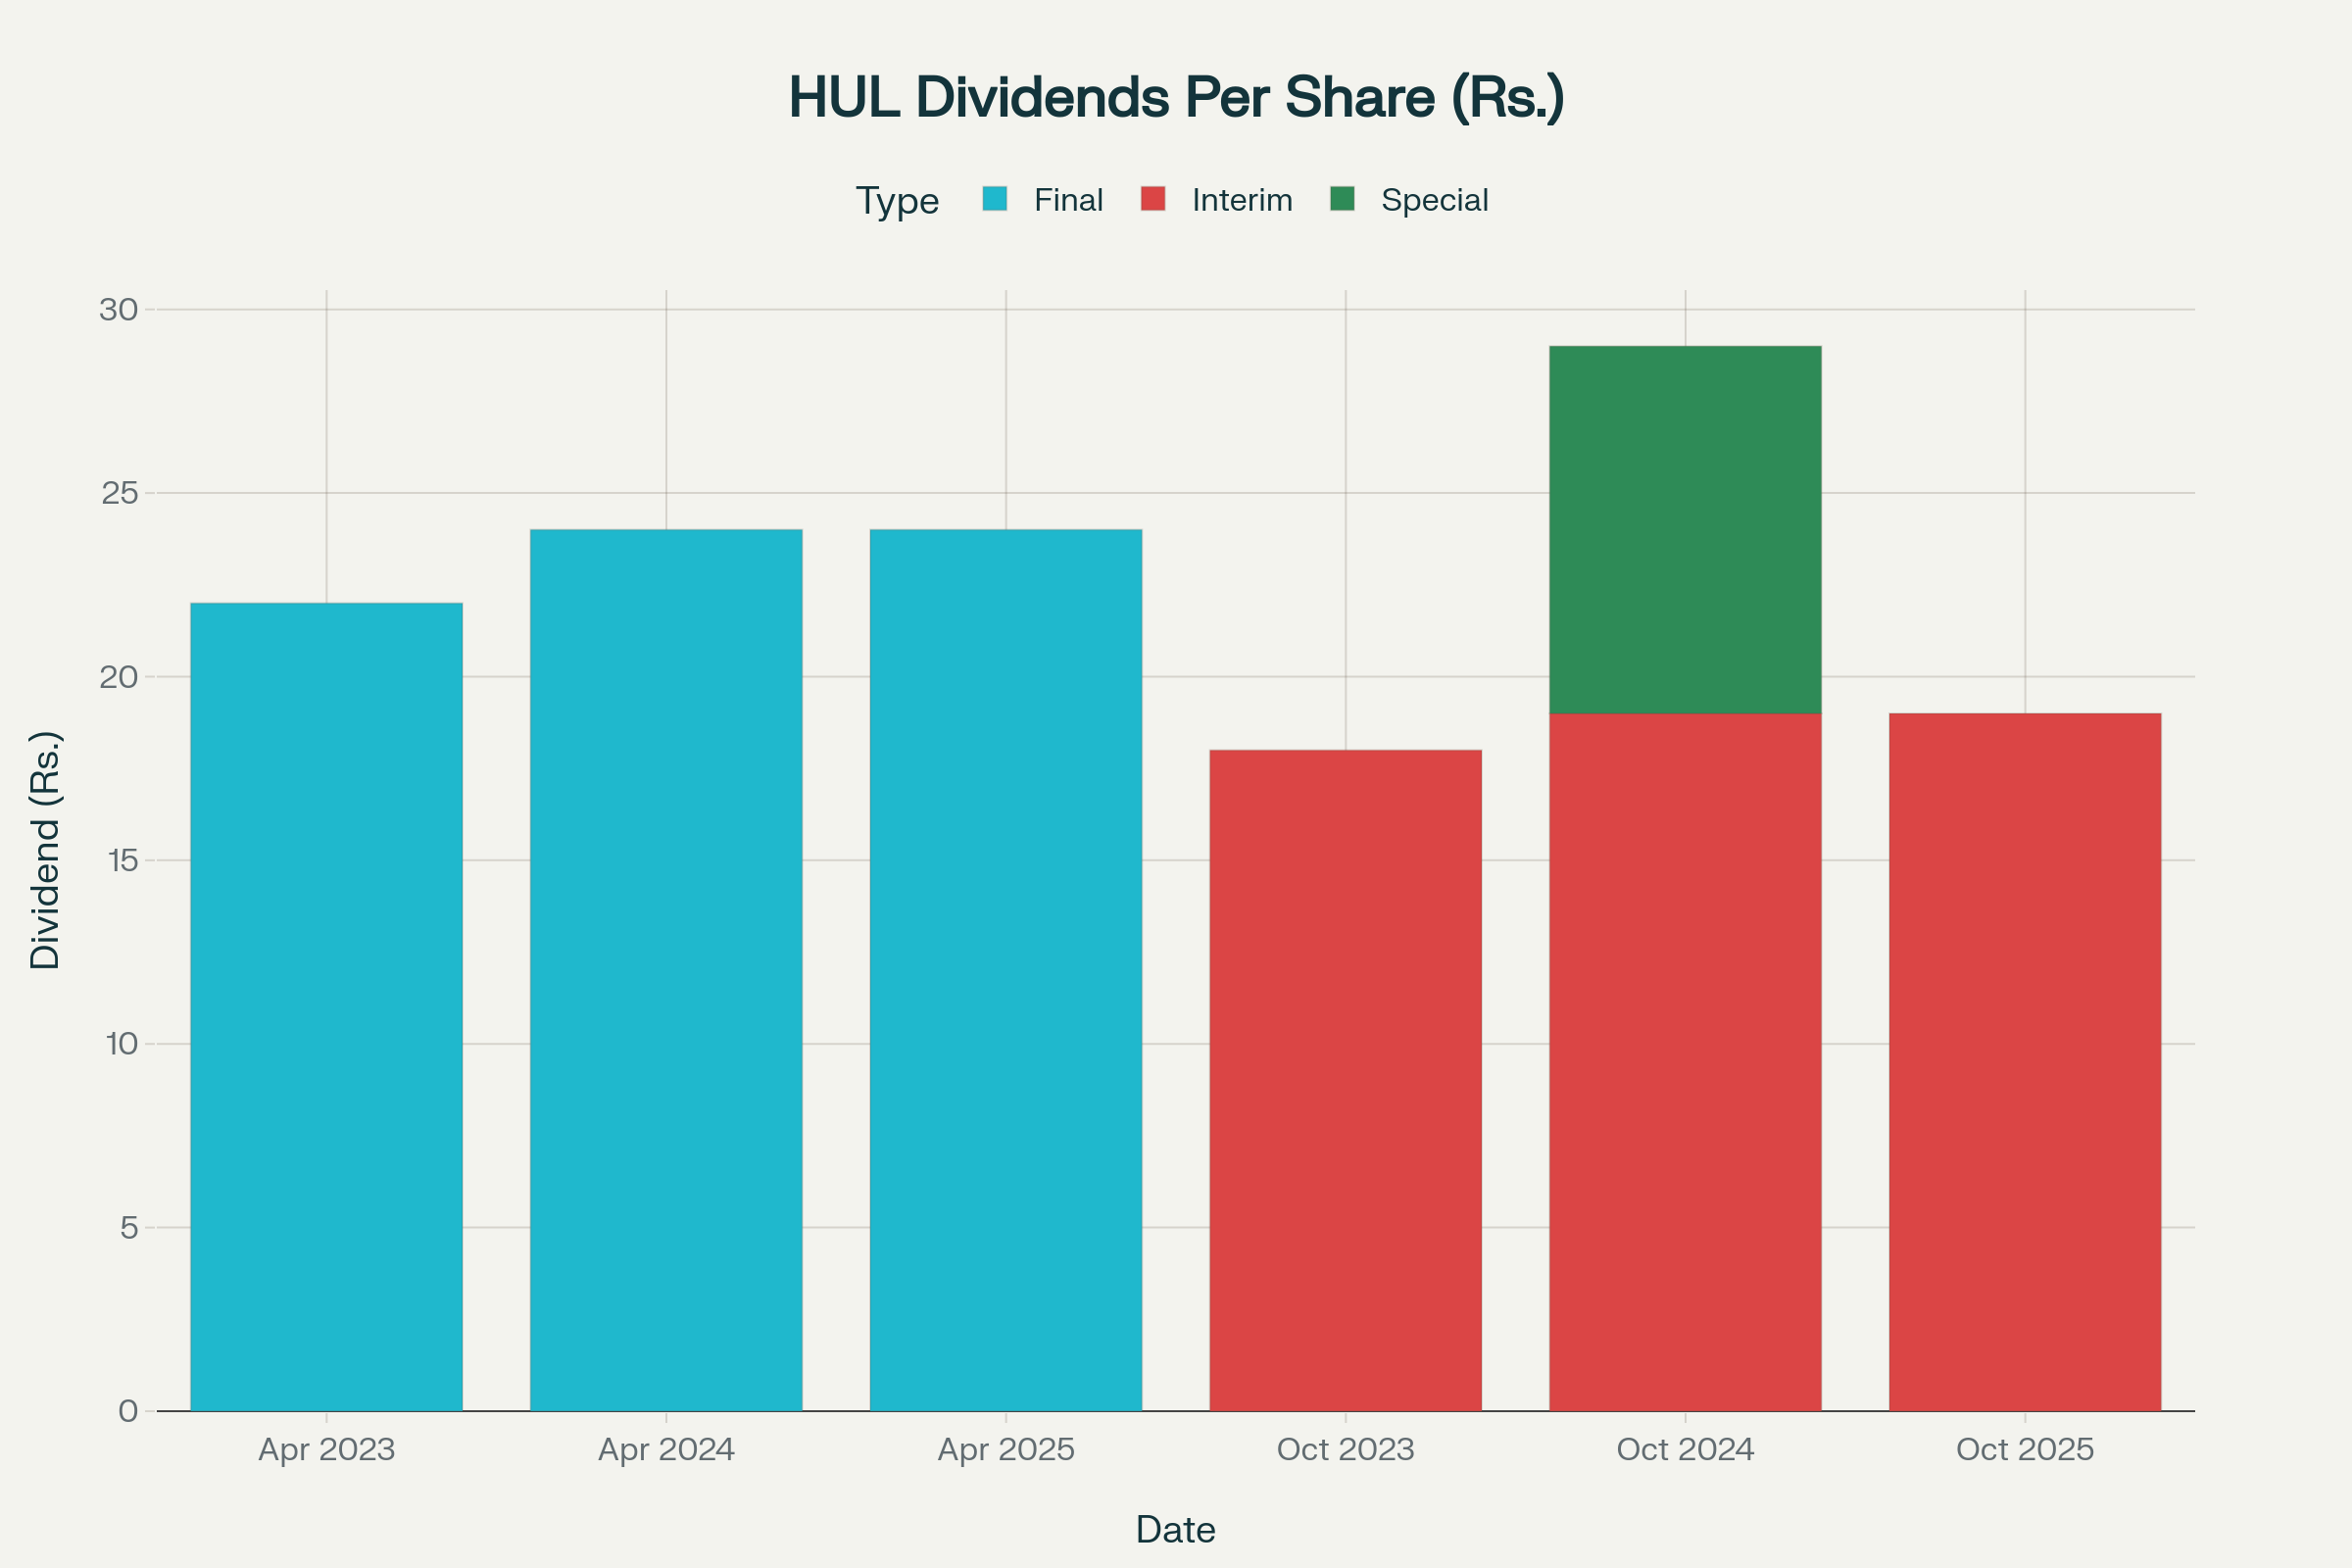
\includegraphics[width=\textwidth]{assets/Dividend_Payout_HUL.png}
        \caption{HUL Dividend Per Share (Rs.)}
    \end{minipage}
    \hfill
    \begin{minipage}{0.48\textwidth}
        \centering
        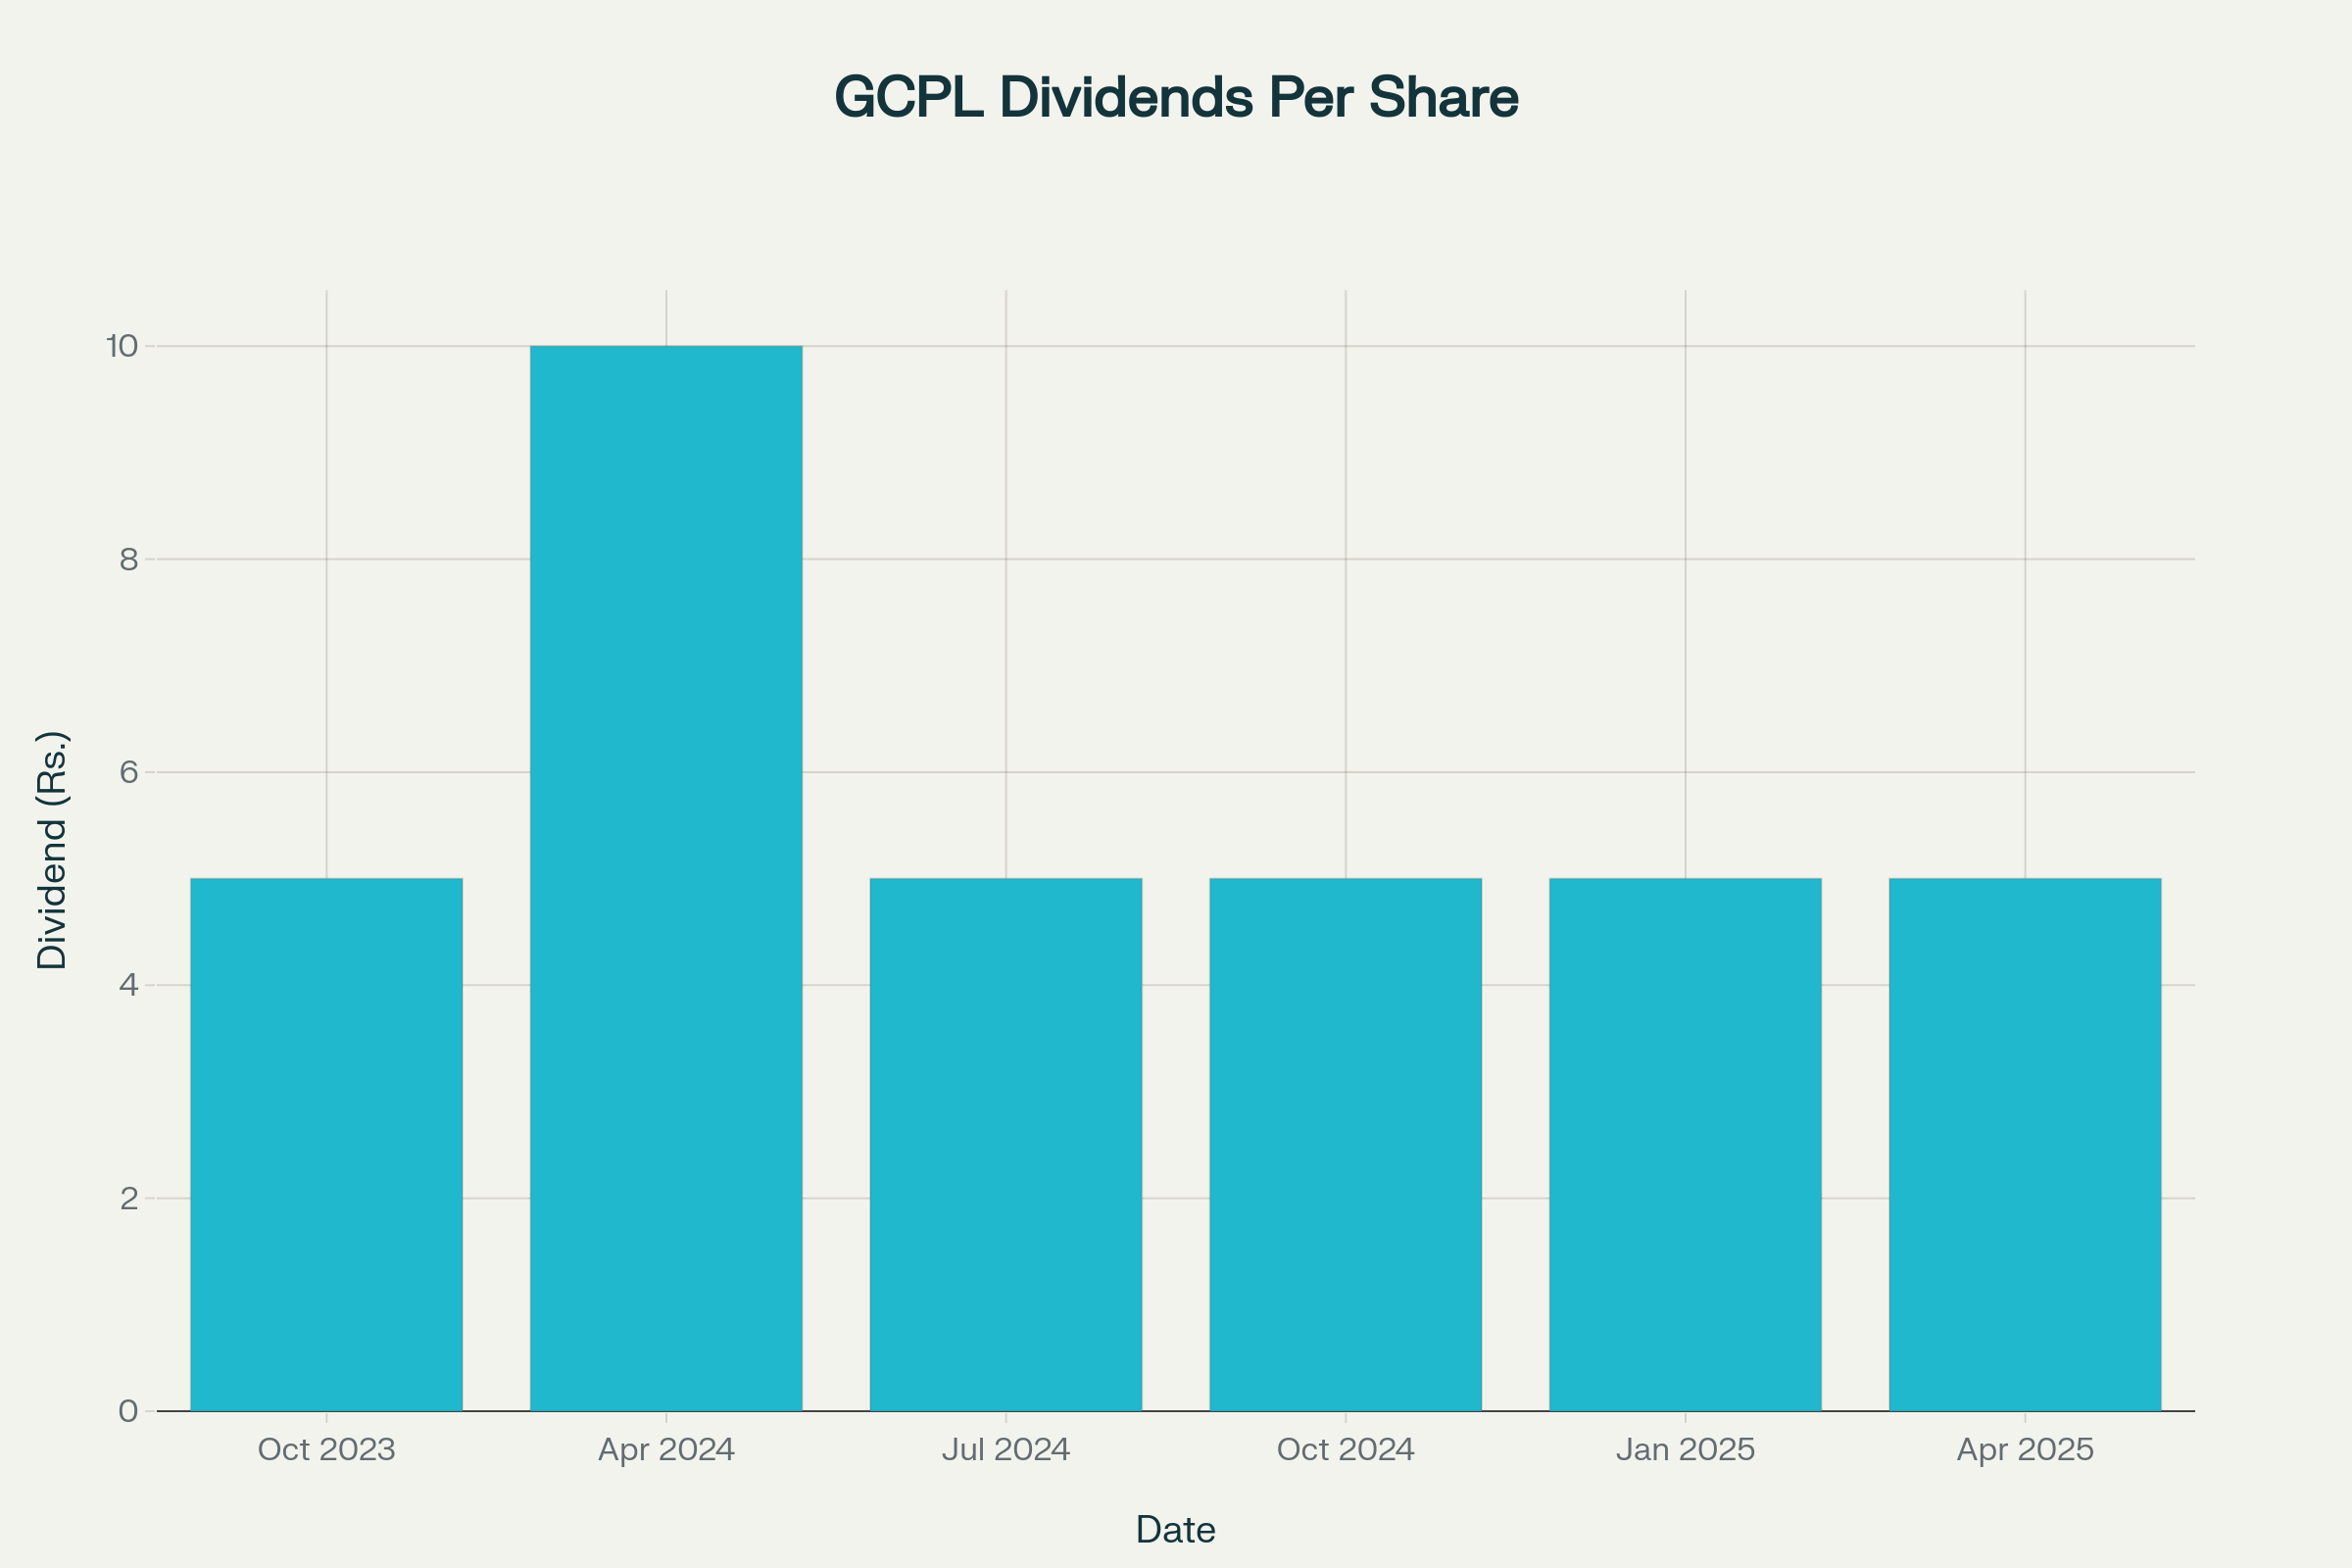
\includegraphics[width=\textwidth]{assets/Dividend_Payout_GCPL.png}
        \caption{GCPL Dividend Per Share (Rs.)}
    \end{minipage}
\end{figure}

\vspace{0.5cm}

\begin{figure}[H]
    \centering
    \begin{minipage}{0.48\textwidth}
        \centering
        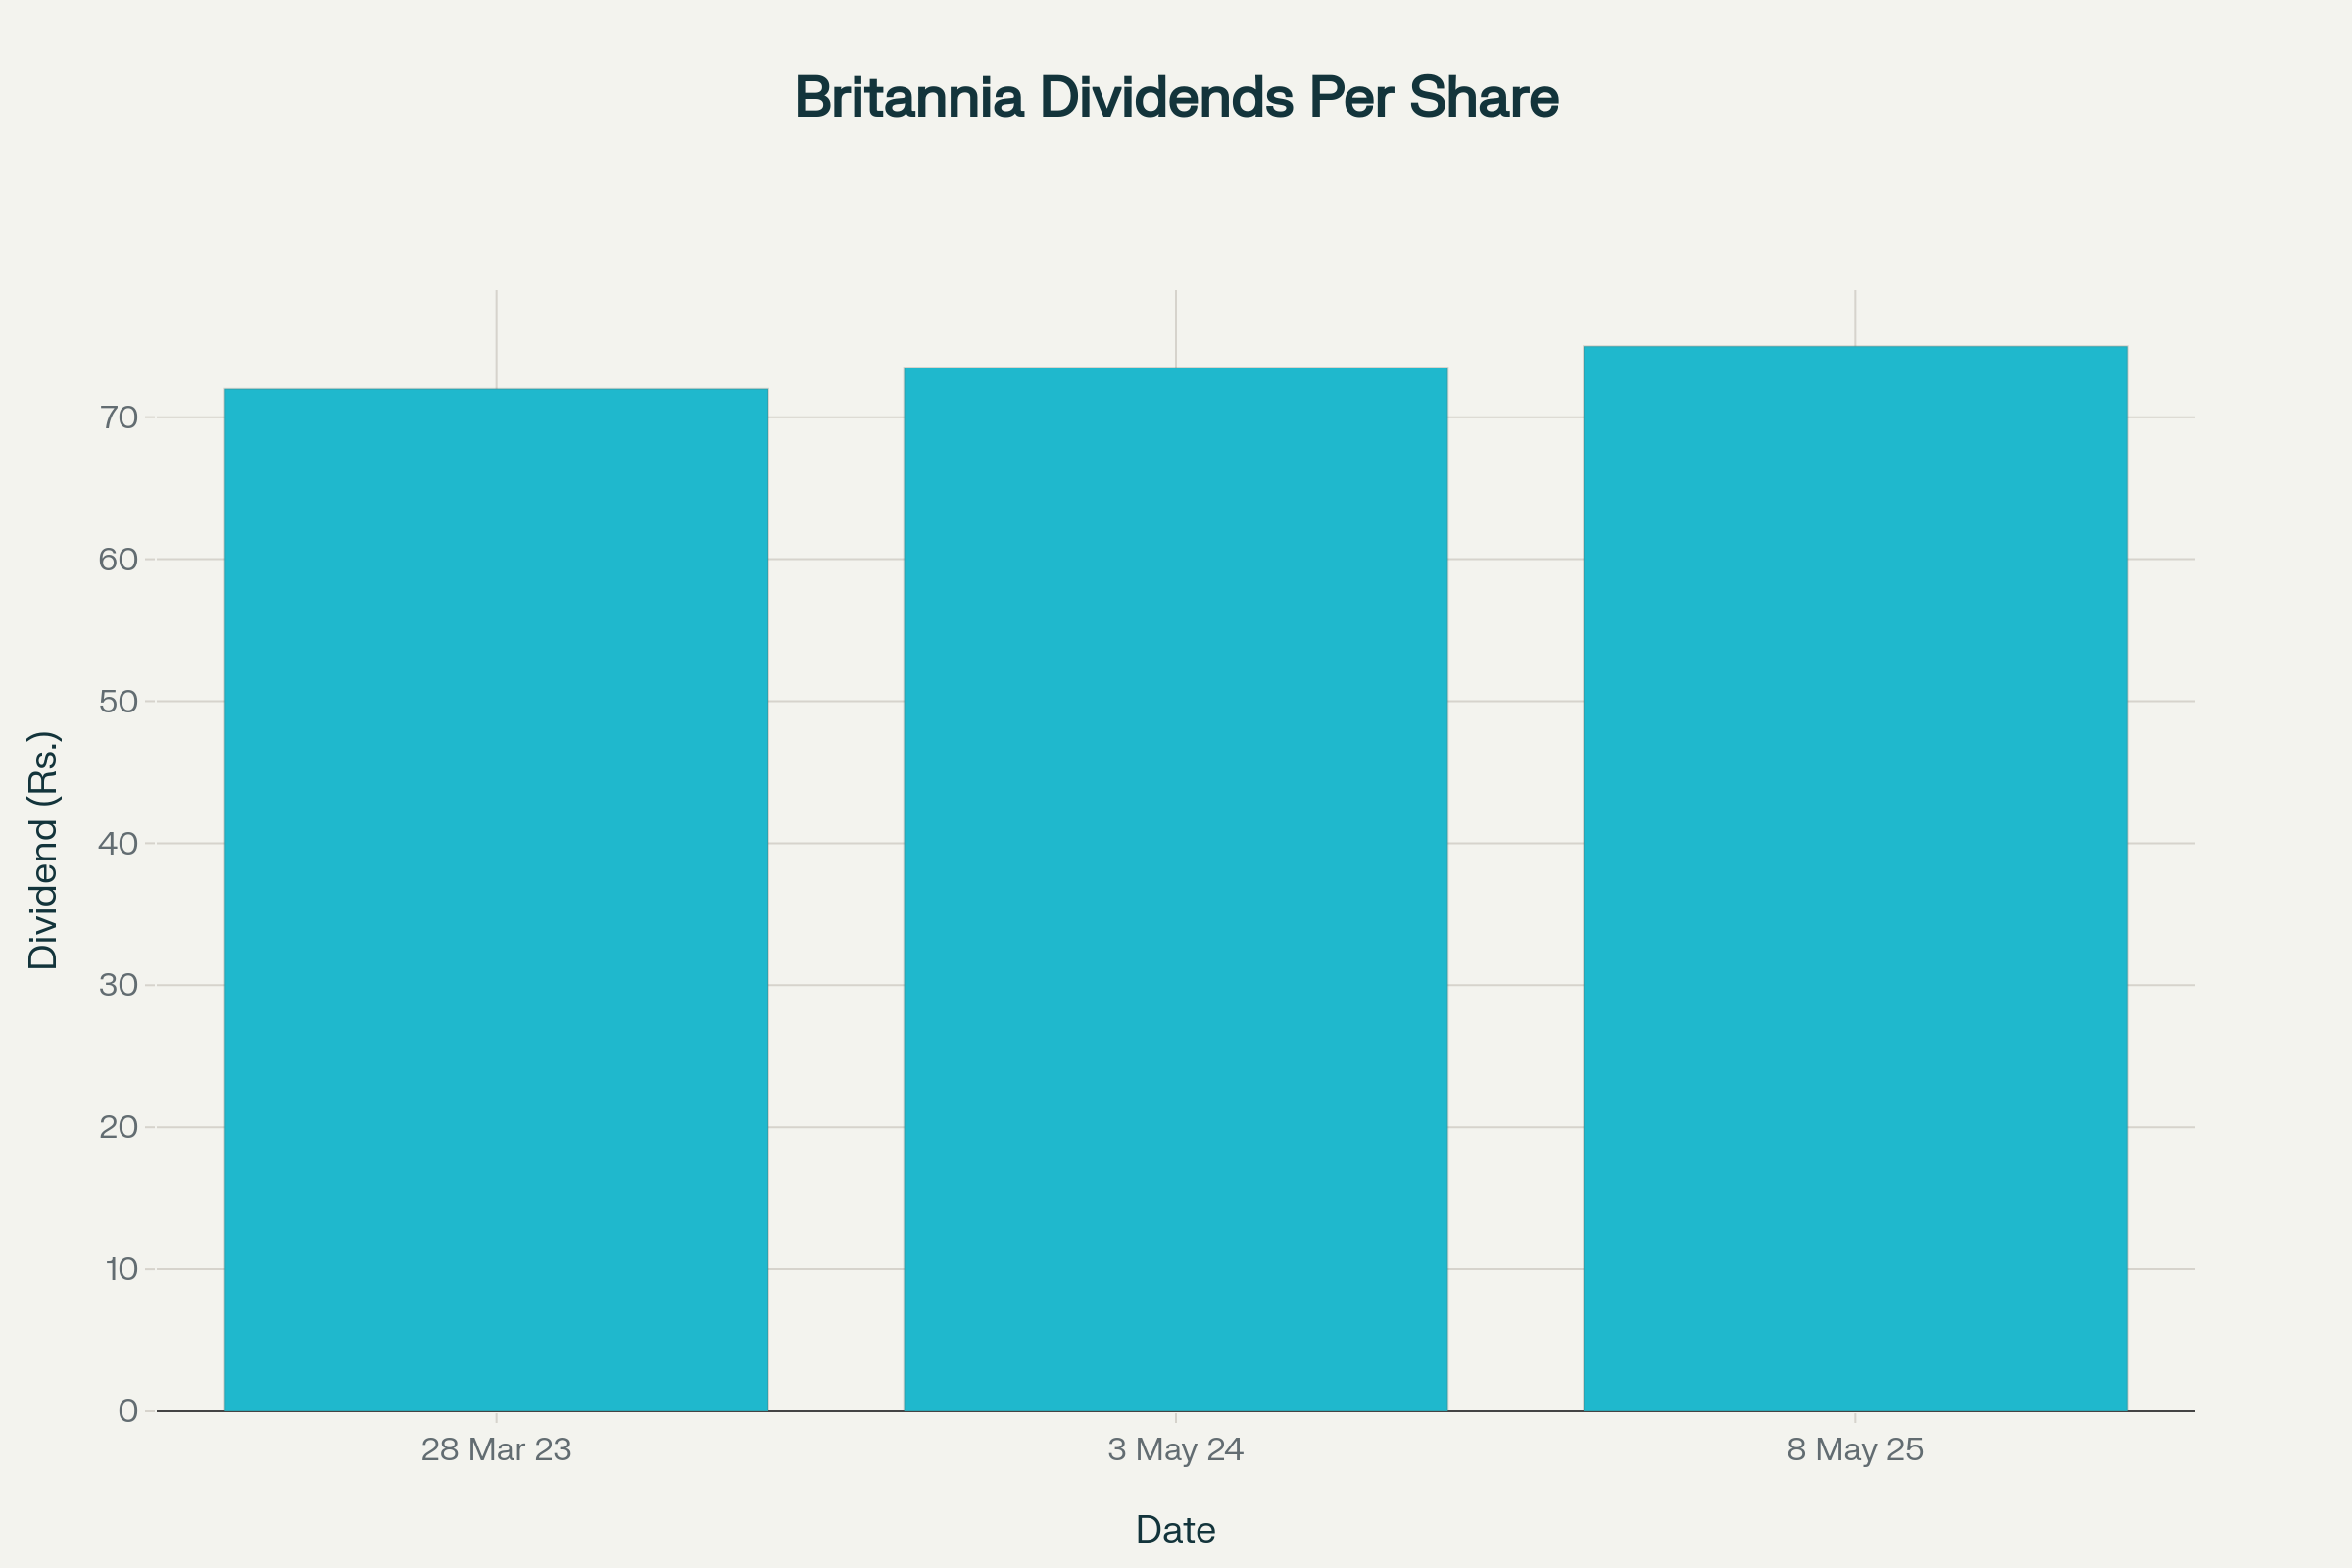
\includegraphics[width=\textwidth]{assets/Dividend_Payout_Britania.png}
        \caption{Britannia Dividend Per Share (Rs.)}
    \end{minipage}
    \hfill
    \begin{minipage}{0.48\textwidth}
        \centering
        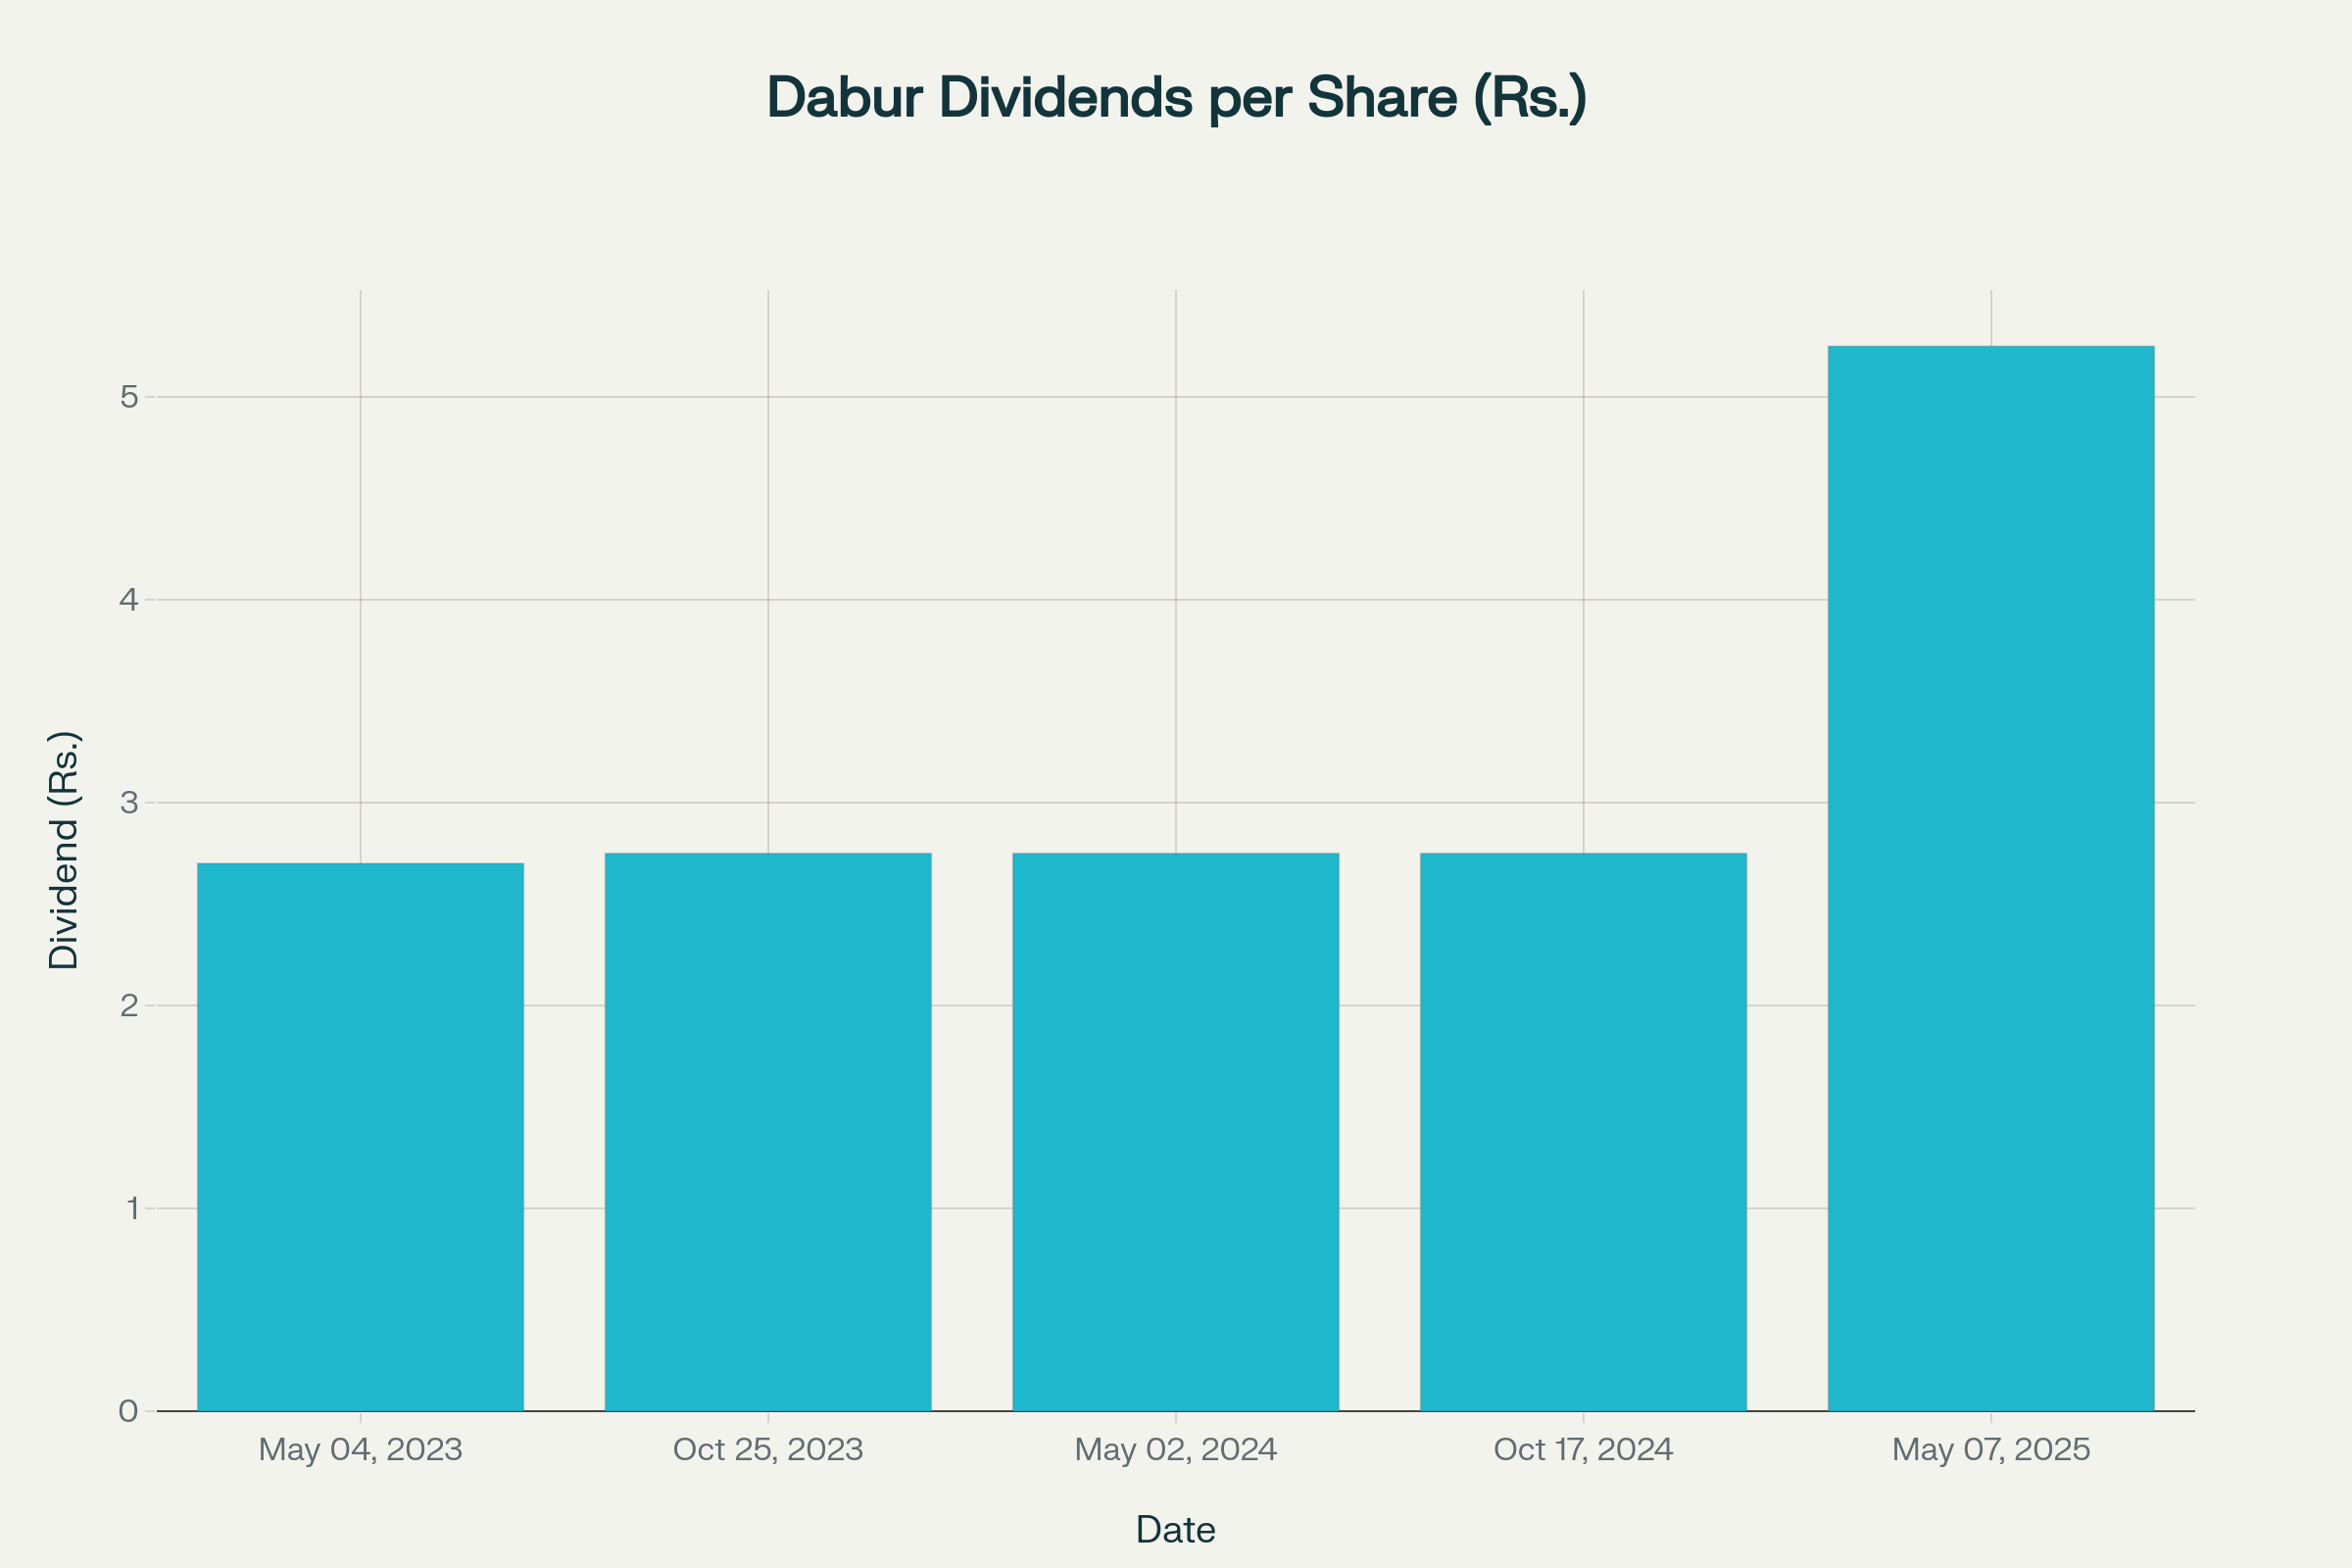
\includegraphics[width=\textwidth]{assets/Dividend_Payout_Dabur.png}
        \caption{Dabur Dividend Per Share (Rs.)}
    \end{minipage}
\end{figure}

\vspace{0.5cm}

\subsection*{Tata Consumer Products and ITC}

\begin{figure}[H]
    \centering
    \begin{minipage}{0.48\textwidth}
        \centering
        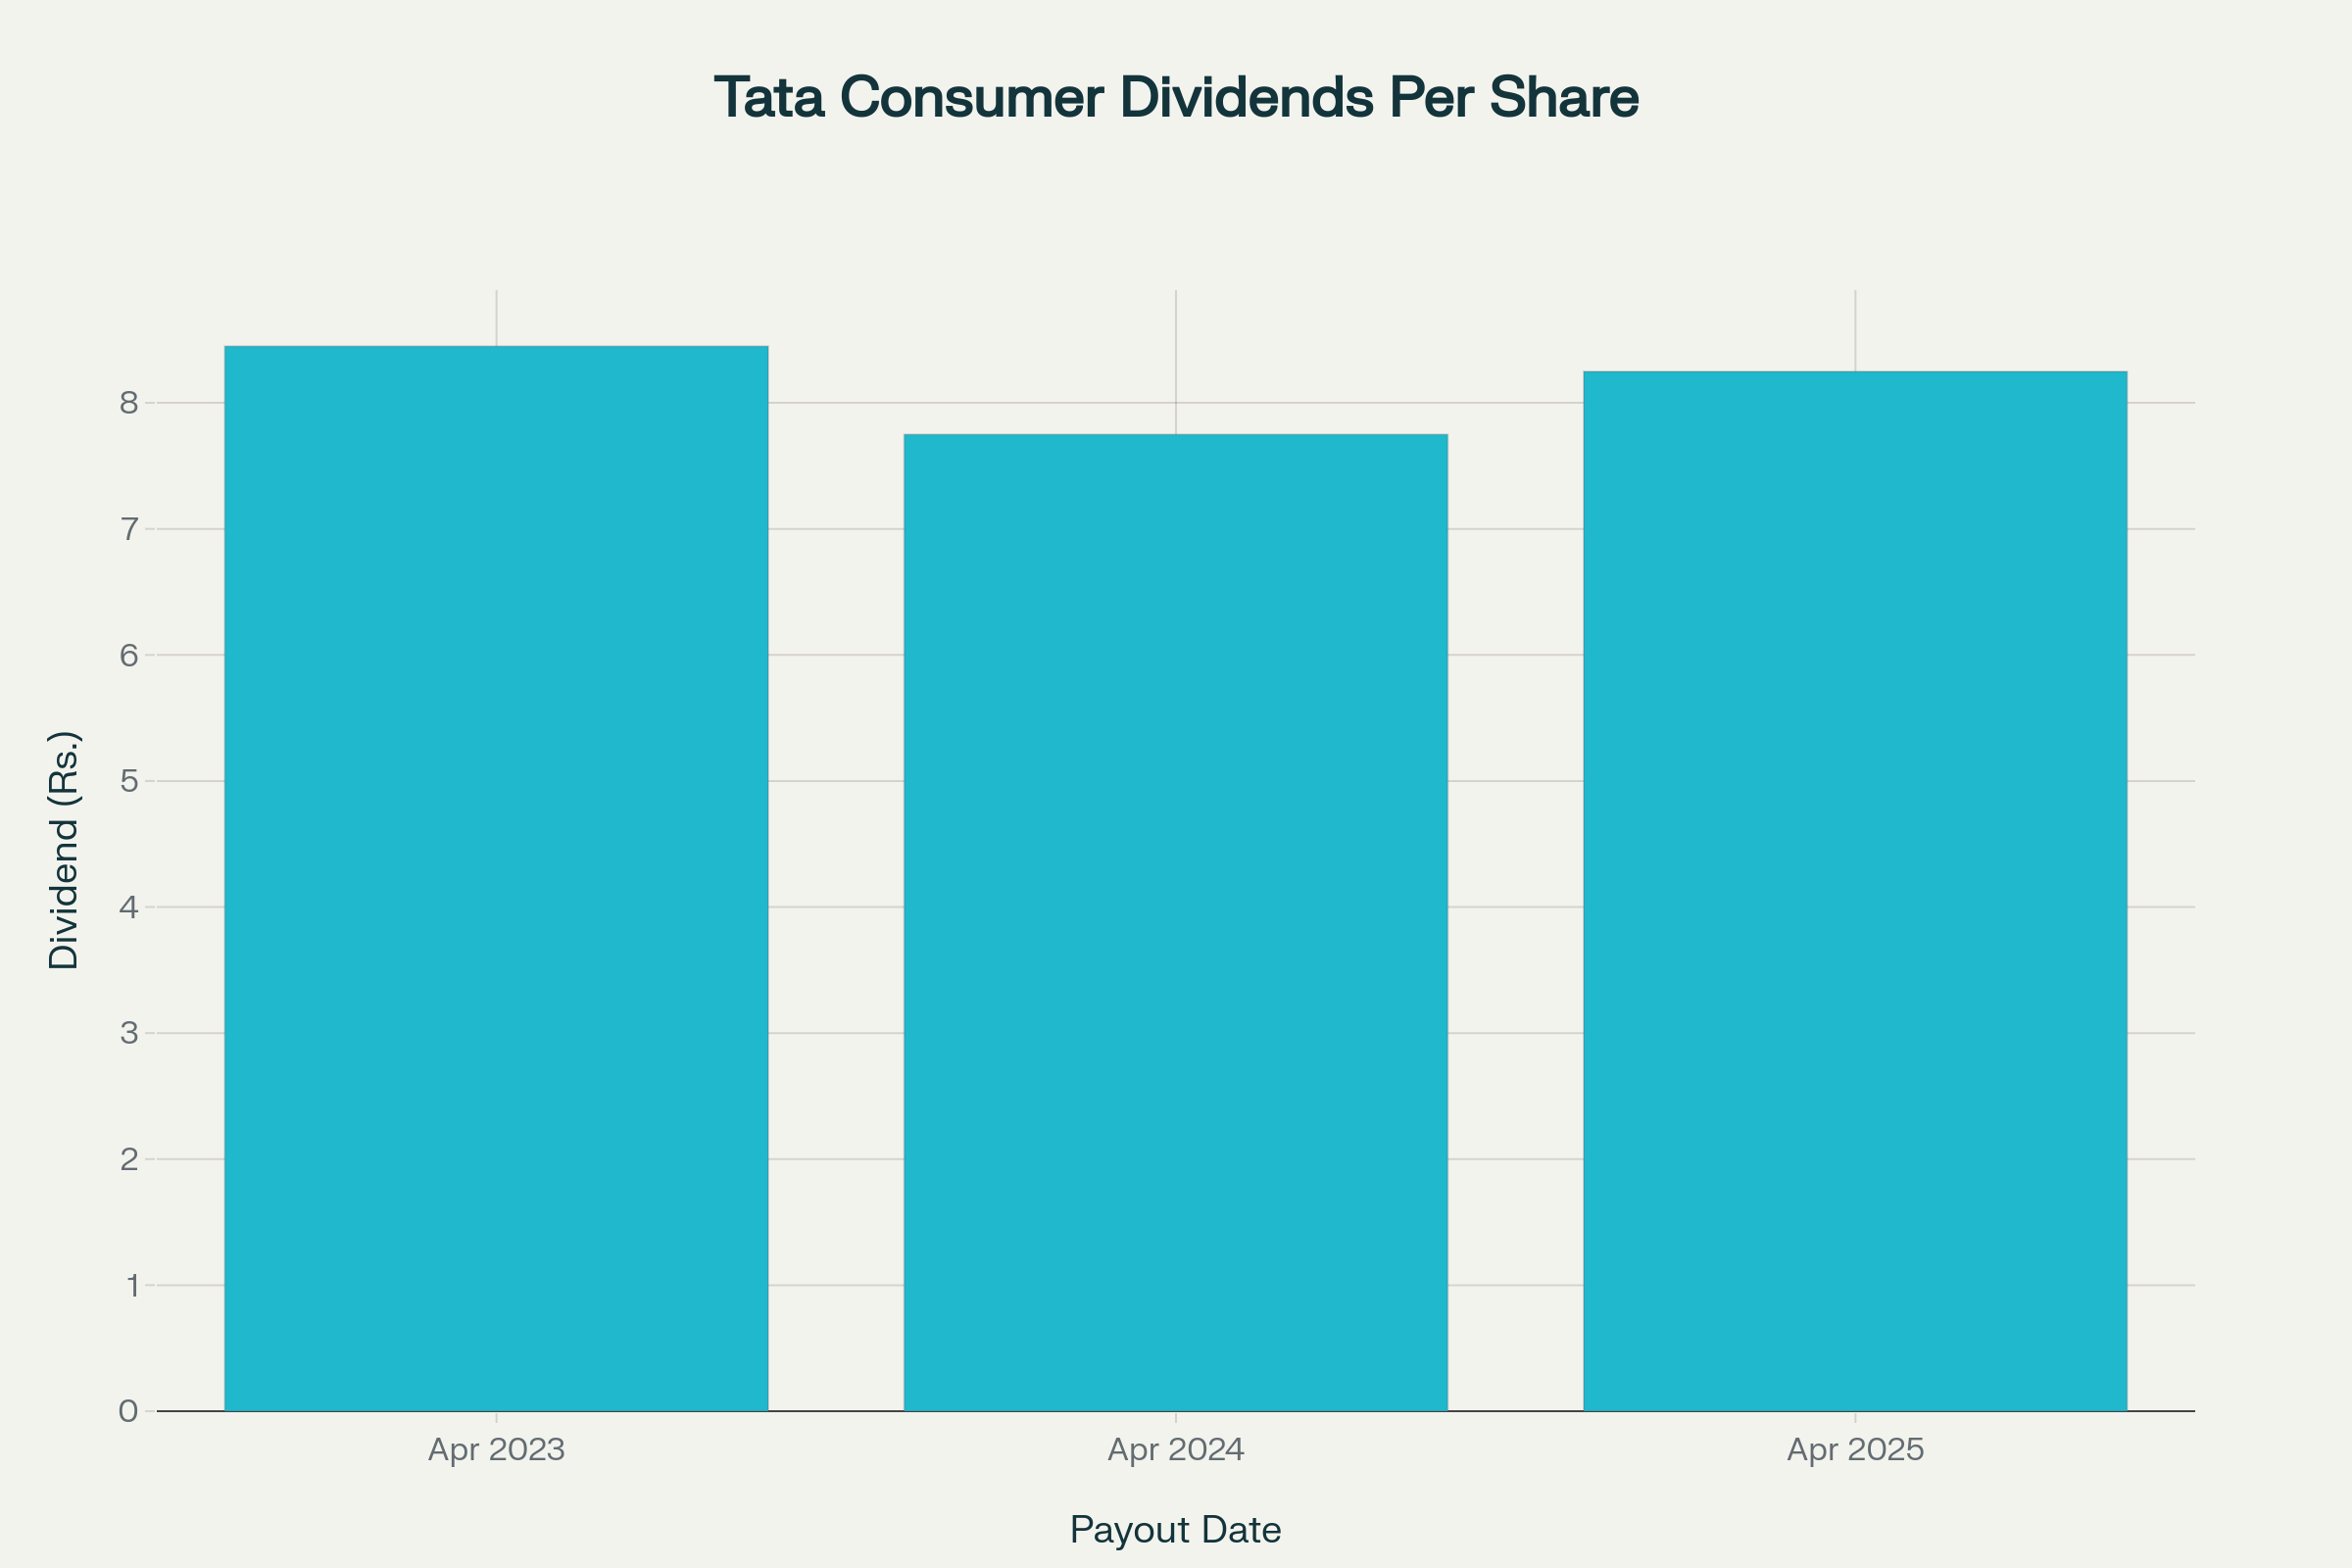
\includegraphics[width=\textwidth]{assets/Dividend_Payout_Tata.png}
        \caption{Tata Consumer Products Dividend Per Share (Rs.)}
    \end{minipage}
    \hfill
    \begin{minipage}{0.48\textwidth}
        \centering
        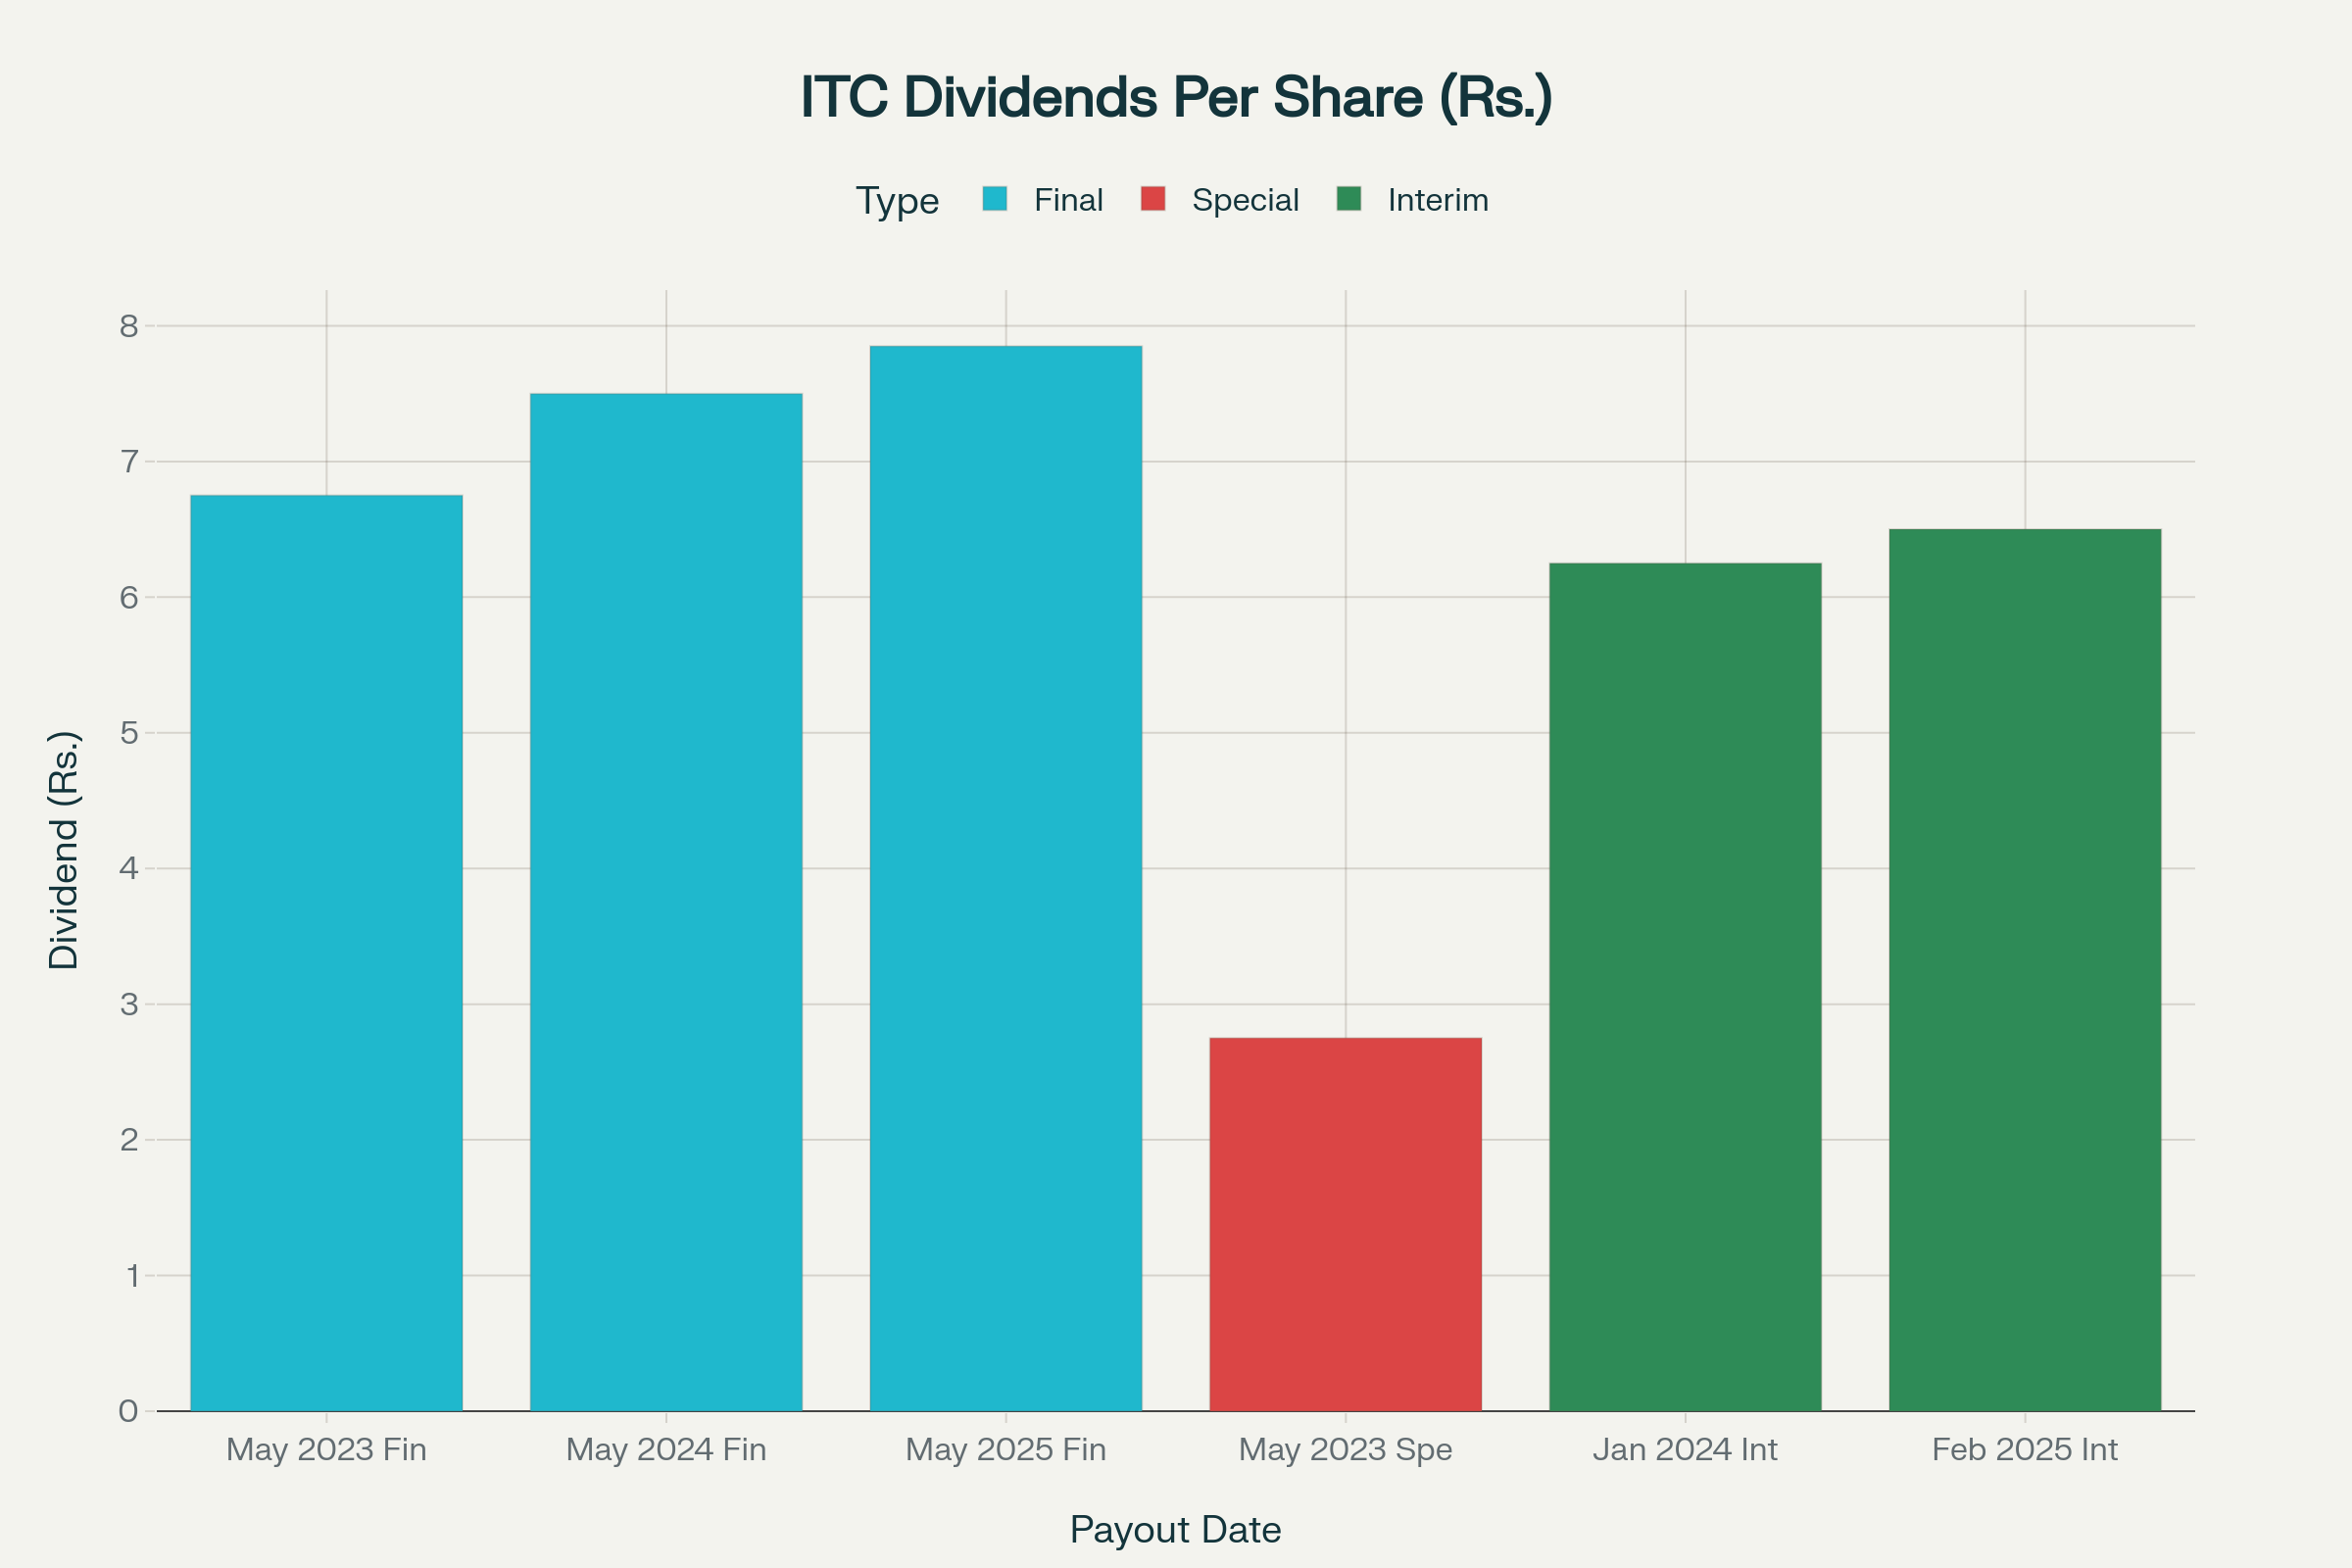
\includegraphics[width=\textwidth]{assets/Dividend_Payout_ITC.png}
        \caption{ITC Dividend Per Share (Rs.)}
    \end{minipage}
\end{figure}


\chapter{Industry Profile: Indian FMCG Sector}

\section{Market Sector and Industry Identification}

\subsection{Market Sector (Broad)}
Consumer Staples (also known as Fast-Moving Consumer Goods or FMCG).

\subsection{Industry (Specific)}
Diversified FMCG. This is the most accurate term as the selected companies operate across multiple categories, including Food \& Beverages, Personal Care, Home Care, and Health \& Wellness.

\subsection{What Qualifies a Company for this Industry?}

Companies in this industry are bound by a common set of characteristics related to their products, market, regulations, and economic sensitivities.

\section{Characteristics Binding the Industry}

\subsection{A. Similar Products and Services}

The core of the industry is selling high-volume, low-margin products that are repurchased frequently and have a short shelf life.

\begin{itemize}
    \item \textbf{HUL:} Dominant in Home Care (Surf Excel, Vim), Beauty \& Personal Care (Dove, Lux, Ponds), and Foods (Knorr, Kissan).
    
    \item \textbf{ITC:} A diversified conglomerate with a core FMCG business (Aashirvaad, Sunfeast, Bingo, Yippee), alongside a significant presence in Tobacco, Hotels, and Paperboards.
    
    \item \textbf{Tata Consumer Products:} Primarily a Beverages \& Foods company (Tata Tea, Tetley, Tata Salt, Tata Sampann). It has recently expanded aggressively into a broader ``pantry platform'' with acquisitions like Capital Foods (Ching's Secret) and Organic India.
    
    \item \textbf{Dabur:} Focuses on health and wellness, built on an Ayurvedic/Natural platform. Key categories include Health (Dabur Chyawanprash), Oral Care (Dabur Red), Hair Care (Vatika), and Foods (Real).
    
    \item \textbf{Britannia:} A market leader in the Bakery \& Dairy category, with iconic brands like Good Day, NutriChoice, and Marie Gold.
    
    \item \textbf{GCPL (Godrej):} A focused player in Home Care (Good Knight) and Personal Care (Cinthol, BBlunt), with a strong presence in emerging markets outside India.
\end{itemize}

\subsection{B. Similar Market}

All six companies target a broad mass-market of over a billion Indian consumers. Their success depends on:

\begin{itemize}
    \item \textbf{Extensive Distribution:} A deep and wide distribution network is non-negotiable, covering everything from traditional kirana (local grocery) stores to modern supermarkets and e-commerce.
    
    \item \textbf{High Brand-Building Costs:} The market is intensely competitive. High advertising and marketing expenditure is essential to build and maintain brand loyalty.
    
    \item \textbf{Growing Digital Channels:} E-commerce and ``Quick Commerce'' (10-minute delivery) are a new, disruptive, and rapidly growing battleground for all players.
\end{itemize}

\subsection{C. Similar Regulations}

These companies operate under a strict common regulatory framework:

\begin{itemize}
    \item \textbf{Food Safety (FSSAI):} The Food Safety and Standards Authority of India governs food product safety, hygiene, licensing, and manufacturing.
    
    \item \textbf{Packaging \& Labeling (Legal Metrology Act):} This act mandates strict rules for packaging declarations, including Maximum Retail Price (MRP), manufacturing date, net weight, and ingredients.
    
    \item \textbf{Advertising (ASCI):} The Advertising Standards Council of India monitors misleading claims, a critical area in a marketing-driven industry.
    
    \item \textbf{Environmental Laws:} The Plastic Waste Management (PWM) Rules put increasing pressure on all players to manage their packaging footprint through recycling and extended producer responsibility (EPR).
    
    \item \textbf{Taxation (GST):} All products fall under the Goods and Services Tax, with different slabs for essential vs. luxury goods.
\end{itemize}

\subsection{D. Similar Economic Response}

The sector is generally ``defensive'' because its products are non-discretionary (people always need soap and salt). However, its performance is highly sensitive to specific economic factors:

\begin{itemize}
    \item \textbf{Rural Demand:} A significant portion of sales comes from rural India. A good monsoon and strong agricultural incomes directly boost rural consumption and, therefore, industry-wide volume.
    
    \item \textbf{Inflation:} The industry is highly sensitive to raw material inflation (e.g., palm oil, crude oil, wheat).
    \begin{itemize}
        \item Company Response: To protect margins, companies either raise prices (price-led growth) or reduce pack sizes (grammage cuts).
        \item Consumer Response: High inflation leads to ``down-trading,'' where consumers shift to cheaper brands or smaller-sized packs (sachets).
    \end{itemize}
    
    \item \textbf{Consumer Sentiment:} When sentiment is positive, ``premiumization'' (buying higher-value products) becomes a key growth driver.
\end{itemize}

\section{Industry Leaders and Laggards}

Industry Leaders include ITC (highest profitability), Britannia (exceptional ROE), and Dabur (strong all-around performer).

Industry Laggards include GCPL and Tata Consumer Products, though they command high P/E ratios suggesting investor optimism for future growth.

\section{Competitive Comparison and Market Dynamics}

\subsection{Stock Performance Analysis (2-Year Trend)}

\begin{figure}[H]
    \centering
    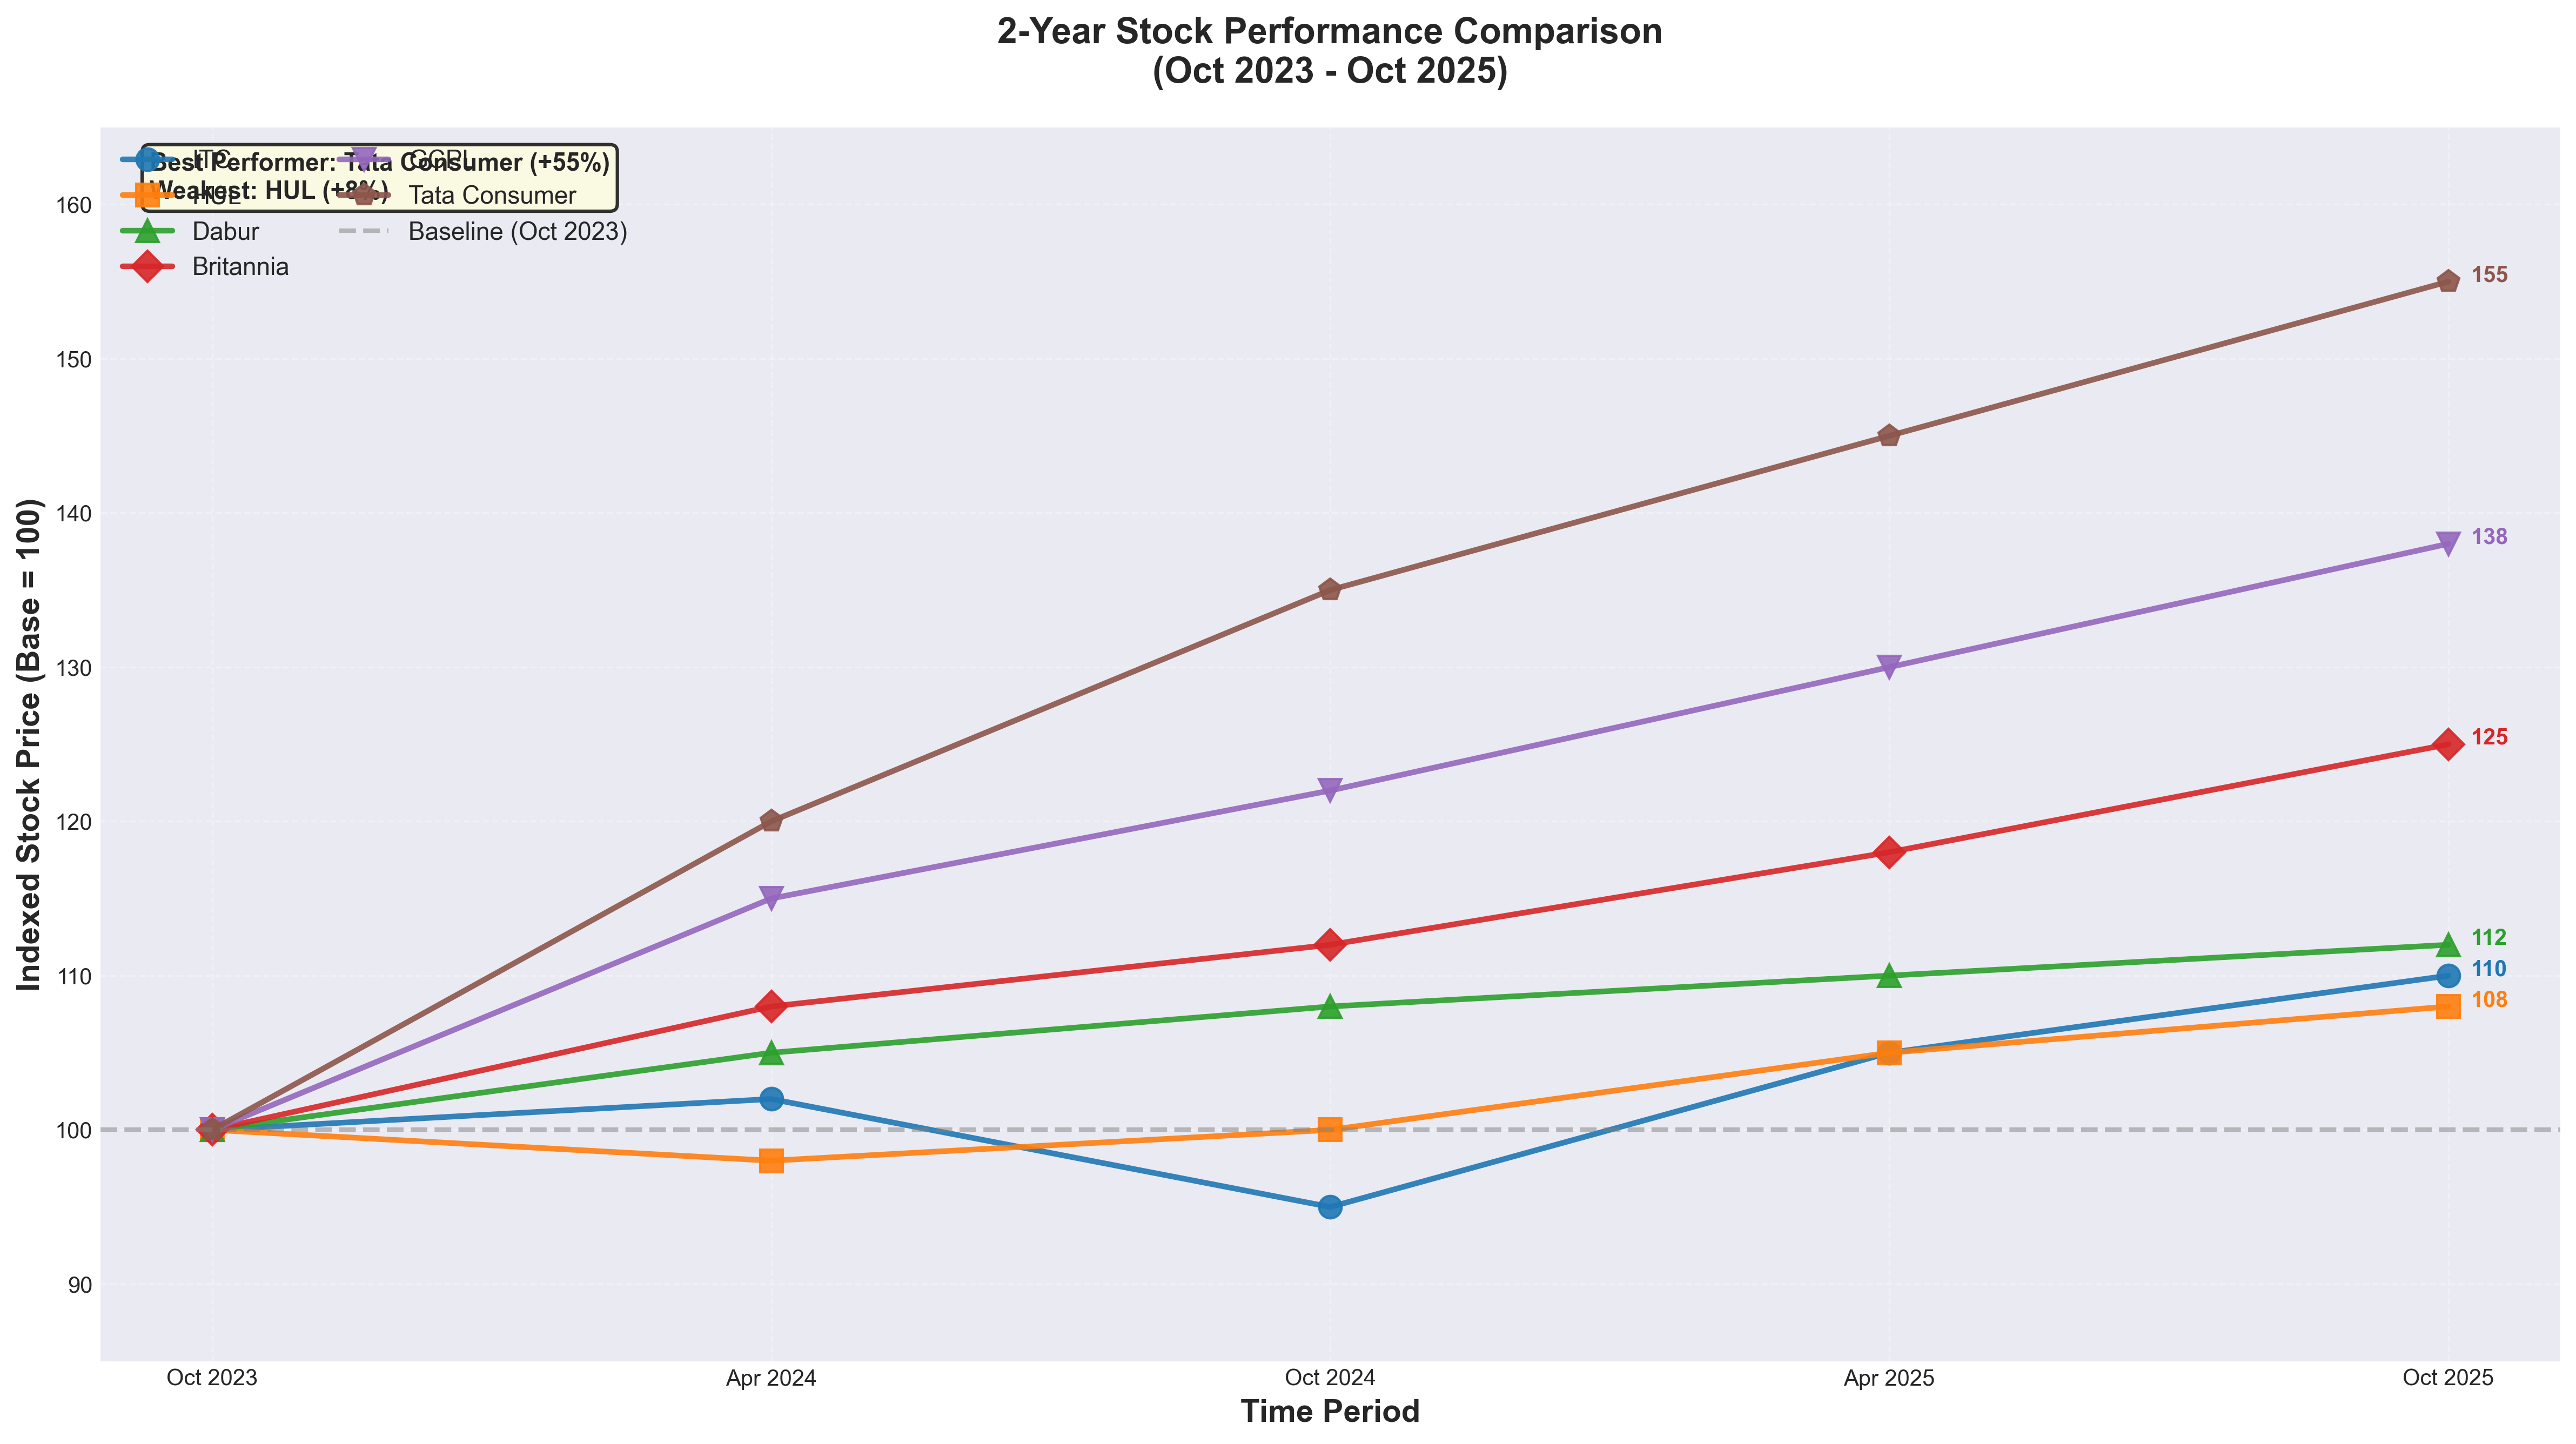
\includegraphics[width=0.85\textwidth]{assets/industry_profile /stock_performance_chart.png}
    \caption{2-Year Stock Performance - Indexed to October 2023 (Base = 100)}
\end{figure}

\subsection{Market Capitalization Distribution}

\begin{figure}[H]
    \centering
    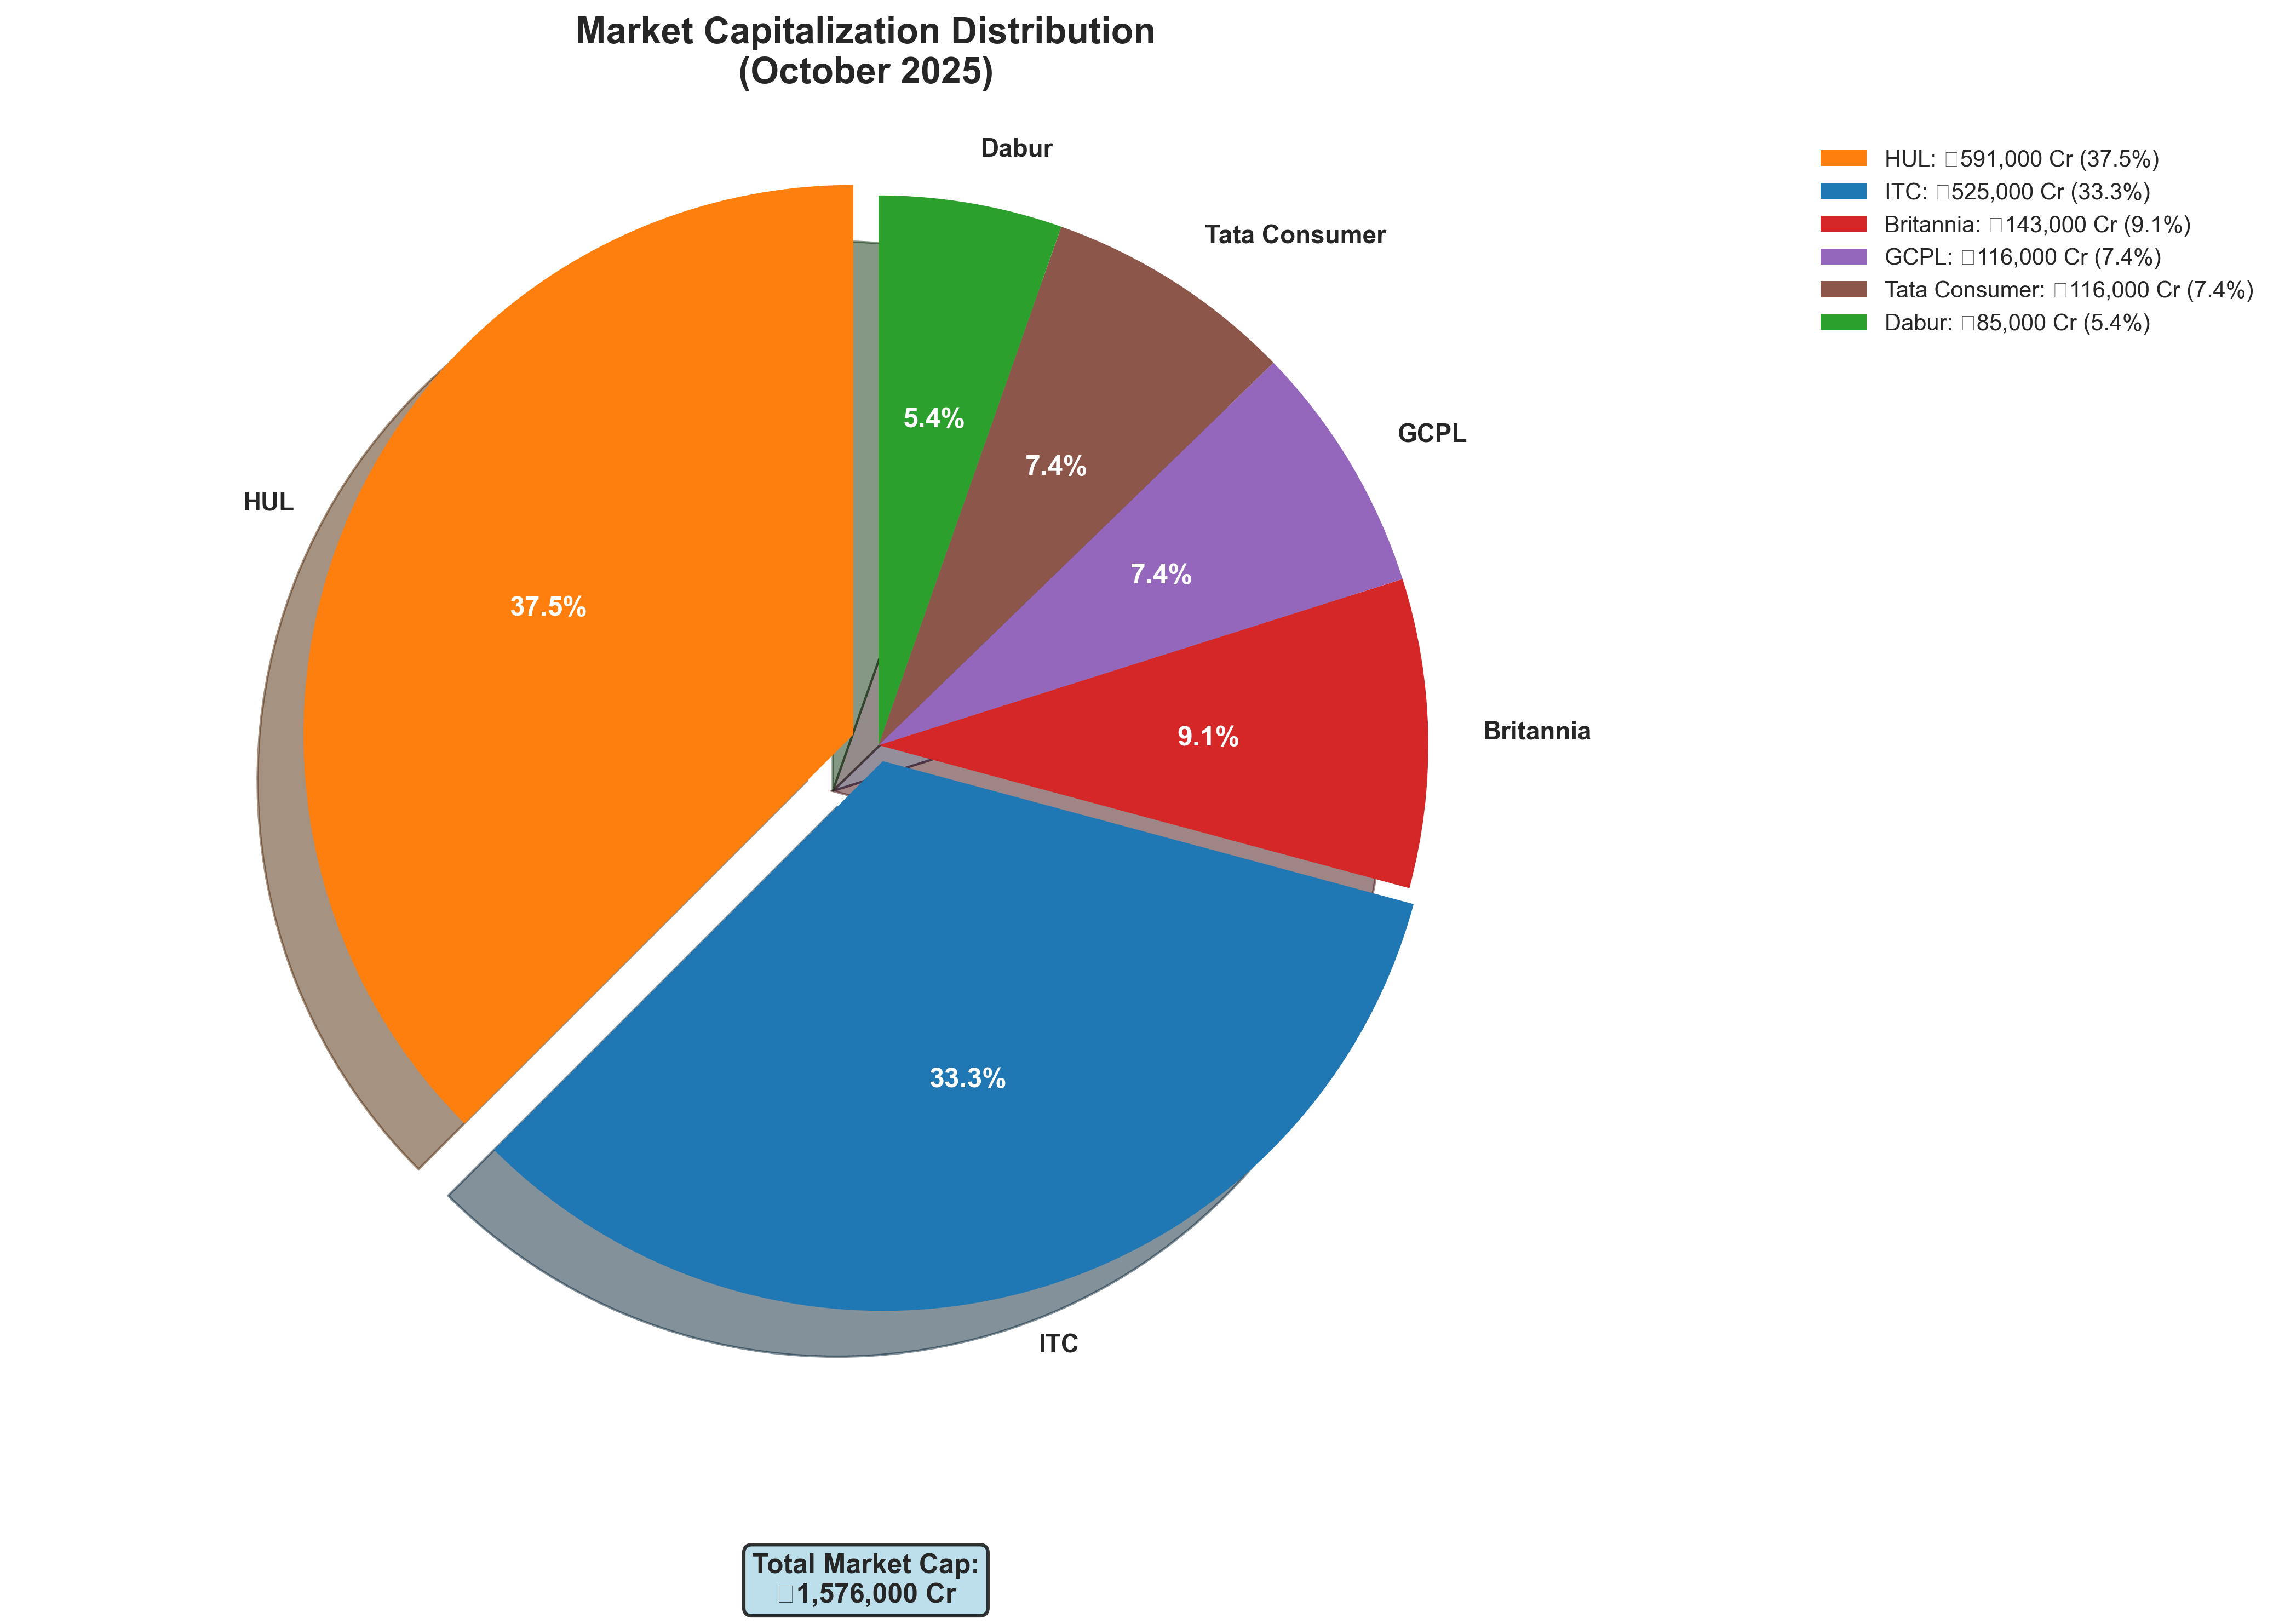
\includegraphics[width=0.85\textwidth]{assets/industry_profile /market_cap_chart.png}
    \caption{Market Capitalization Distribution - October 2025}
\end{figure}

\section{Company Positioning}

\subsection{Tata Consumer Products}

\textbf{Position:} High-growth, high-premium stock. The company's stock surge (+55\%) and extreme P/E ratio (106.53) are completely disconnected from its low 2024 profitability (7.21\% ROE). This is a classic ``growth story'' driven by aggressive acquisition strategy in 2024.

\subsection{ITC}

\textbf{Position:} Mature, high-profit ``value'' stock undergoing transformation. ITC's low P/E (26.13) reflects its legacy as a mature (but highly profitable) tobacco business that pays a high dividend. Stock volatility was event-driven by the demerger of its hotel business.

\subsection{HUL}

\textbf{Position:} The stable, mature market leader. HUL's modest stock growth (+8\%) reflects its maturity, with the company struggling with low volume growth in 2024.

\section{NIFTY FMCG Index}

The NIFTY FMCG index is a sectoral benchmark on the National Stock Exchange of India that tracks the performance of 15 leading companies in the fast-moving consumer goods (FMCG) sector, which includes non-durable and mass-consumption products such as food, beverages, personal care, and household items. 

Calculated using the free float market capitalization method, this index reflects the relative market value of its constituent stocks and serves as a crucial tool for benchmarking, launching ETFs, and structured products. Key constituents include industry giants like Hindustan Unilever, ITC, and Nestlé India, whose steady growth and resilience have ensured the index remains vital for investors and portfolio managers tracking trends in India's rapidly evolving consumer market.

\newpage

% ===============================================
% CHAPTER 4: FINANCIAL STATEMENT ANALYSIS
% ===============================================
\chapter{Financial Statement Analysis}

This report analyzes the financial performance of six major FMCG companies (ITC, HUL, Tata, Dabur, Britannia, and GCPL) across key financial dimensions including liquidity, profitability, leverage, and operational efficiency. The analysis reveals divergent strategic paths: while some companies strengthened their balance sheets through deleveraging, others experienced significant operational challenges requiring deeper investigation.

\section{Liquidity Analysis: Short-Term Financial Health}

\subsection{Strong Performers}

ITC maintains exceptional liquidity with a current ratio of 2.91, improving 2.5\% year-over-year. This positions ITC as the sector leader in short-term solvency, providing substantial cushion to weather market volatility. However, the quick ratio declined 4.8\% to 1.89, suggesting increased inventory levels relative to liquid assets—a concern explored further in operational efficiency metrics.

Dabur demonstrated the most impressive liquidity turnaround, with its current ratio surging 40\% from a concerning 0.85 to 1.19. More remarkably, the quick ratio doubled (106.2\% increase) to 0.79. This transformation suggests aggressive working capital management, potentially through accelerated receivables collection or strategic reduction in short-term liabilities. While still below the 1.5 benchmark, the trajectory indicates improving financial flexibility.

\begin{figure}[H]
    \centering
    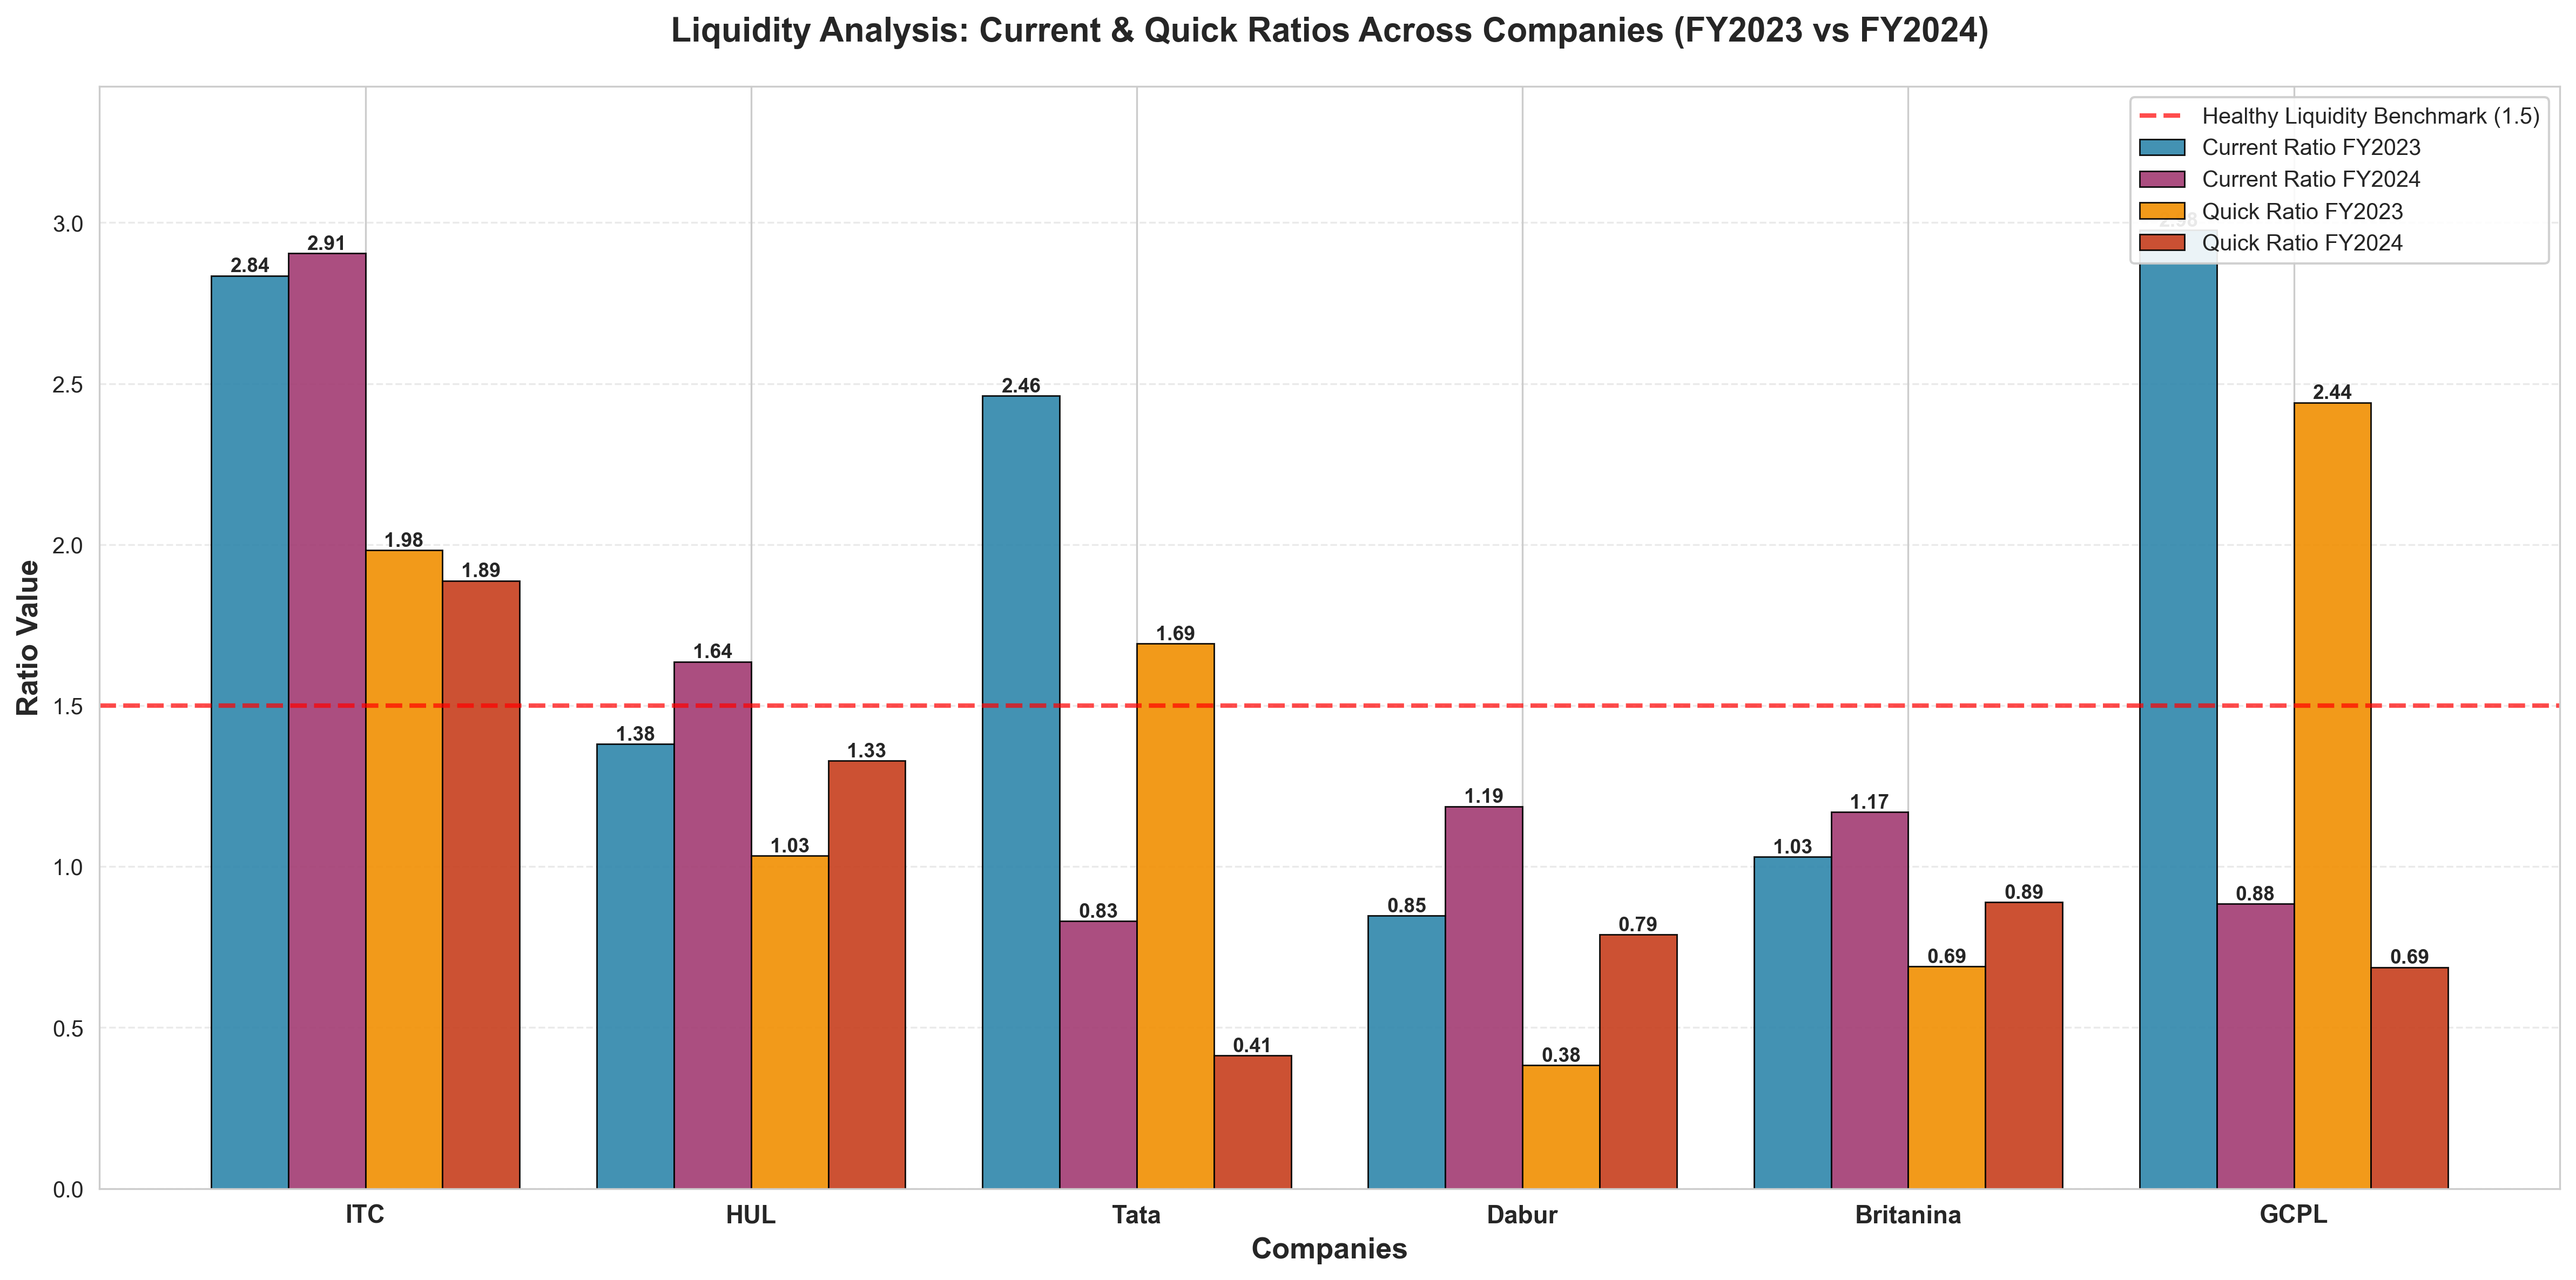
\includegraphics[width=0.8\textwidth]{assets/imperative_analysis/liquidity_analysis.png}
    \caption{Liquidity Analysis - Current and Quick Ratios Comparison}
\end{figure}

\vspace{0.3cm}

GCPL and Tata experienced severe liquidity deterioration that demands immediate management attention. GCPL's current ratio collapsed 70.3\% from 2.98 to 0.88, falling below the critical 1.0 threshold. This dramatic shift, coupled with a 71.8\% decline in quick ratio to 0.69, suggests one of three scenarios: aggressive expansion funded through short-term debt, significant working capital mismanagement, or potential reclassification of liabilities from long-term to short-term.

Tata similarly suffered a 66.2\% liquidity decline (current ratio: 2.46 → 0.83), with quick ratio plummeting 75.6\%. This transformation is particularly alarming given Tata's minimal leverage (D/E: 0.017), suggesting the issue stems from operational factors—possibly inventory buildup or delayed receivables—rather than debt restructuring.

HUL and Britannia occupy the middle ground with modest improvements of 18.6\% and 13.6\% respectively, though both remain below the 1.5 comfort zone at 1.64 and 1.17.

\section{Profitability Analysis: Operational Excellence and Margin Management}

\subsection{Exceptional Performance}

GCPL achieved extraordinary profitability expansion with net profit margin skyrocketing 327.4\% from 17.1\% to 73.0\%. This exceptional jump warrants investigation into whether it reflects: (a) one-time gains from asset sales or restructuring, (b) dramatic cost reduction initiatives, or (c) premium product mix shift. The accompanying 23.9\% gross margin improvement (44.4\% → 55.1\%) suggests genuine operational improvements rather than merely financial engineering, though such extreme growth is unsustainable.

\begin{figure}[H]
    \centering
    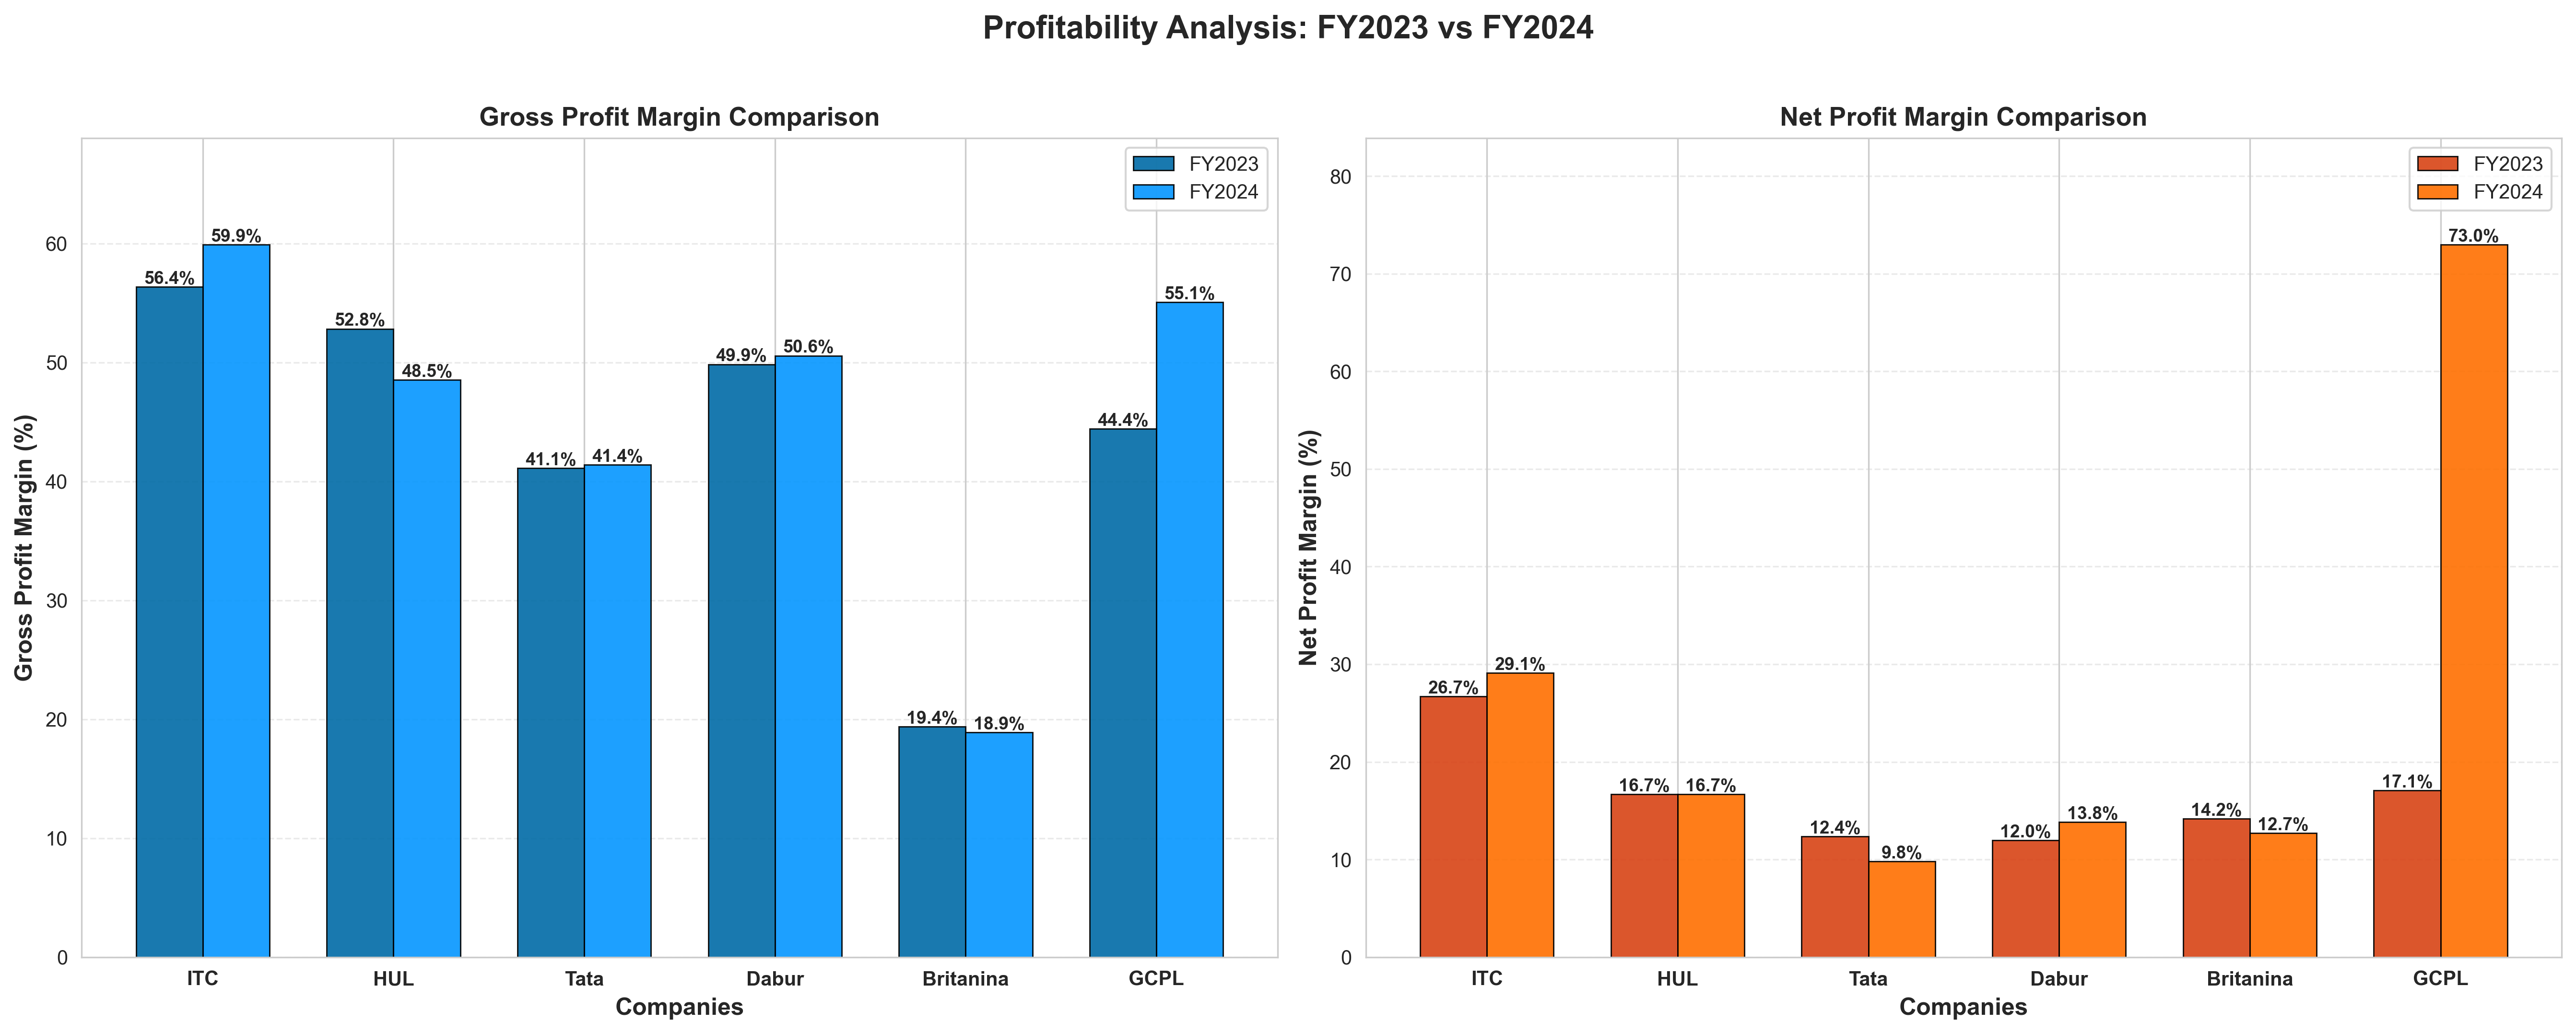
\includegraphics[width=0.8\textwidth]{assets/imperative_analysis/profitability_analysis.png}
    \caption{Profitability Analysis - Net Profit Margins Across Companies}
\end{figure}

\vspace{0.3cm}

Dabur improved net profitability by 15.5\% to 13.8\%, accompanied by modest gross margin expansion of 1.5\%. This balanced improvement suggests effective cost management throughout the value chain rather than dependence on top-line pricing actions alone.

\subsection{Profitability Pressures}

Tata experienced significant msargin compression with net profit declining 20.8\% to 9.8\%, despite maintaining stable gross margins (41.1\% → 41.4\%). This divergence between gross and net margins indicates escalating operating expenses or interest costs consuming the gross profit. The stable gross margin rules out raw material inflation or pricing pressure, pointing instead to SG\&A bloat, increased depreciation, or expansion-related expenses.

Britannia faced a 10.6\% net margin decline to 12.7\%, coupled with a 2.6\% gross margin contraction. This suggests dual pressures: input cost inflation eroding gross profitability, compounded by additional operating expense burdens. As a biscuit manufacturer, Britannia faces direct exposure to wheat, sugar, and palm oil price volatility.

HUL presents an interesting case with net margins remaining virtually flat at 16.7\% (+0.2\%), despite an 8.2\% gross margin decline (52.8\% → 48.5\%). This stability amid gross margin compression indicates aggressive operating expense management, likely reflecting restructuring initiatives, distribution efficiency gains, or reduced marketing spend—a potentially risky trade-off between short-term profitability and long-term brand equity.

\begin{figure}[H]
    \centering
    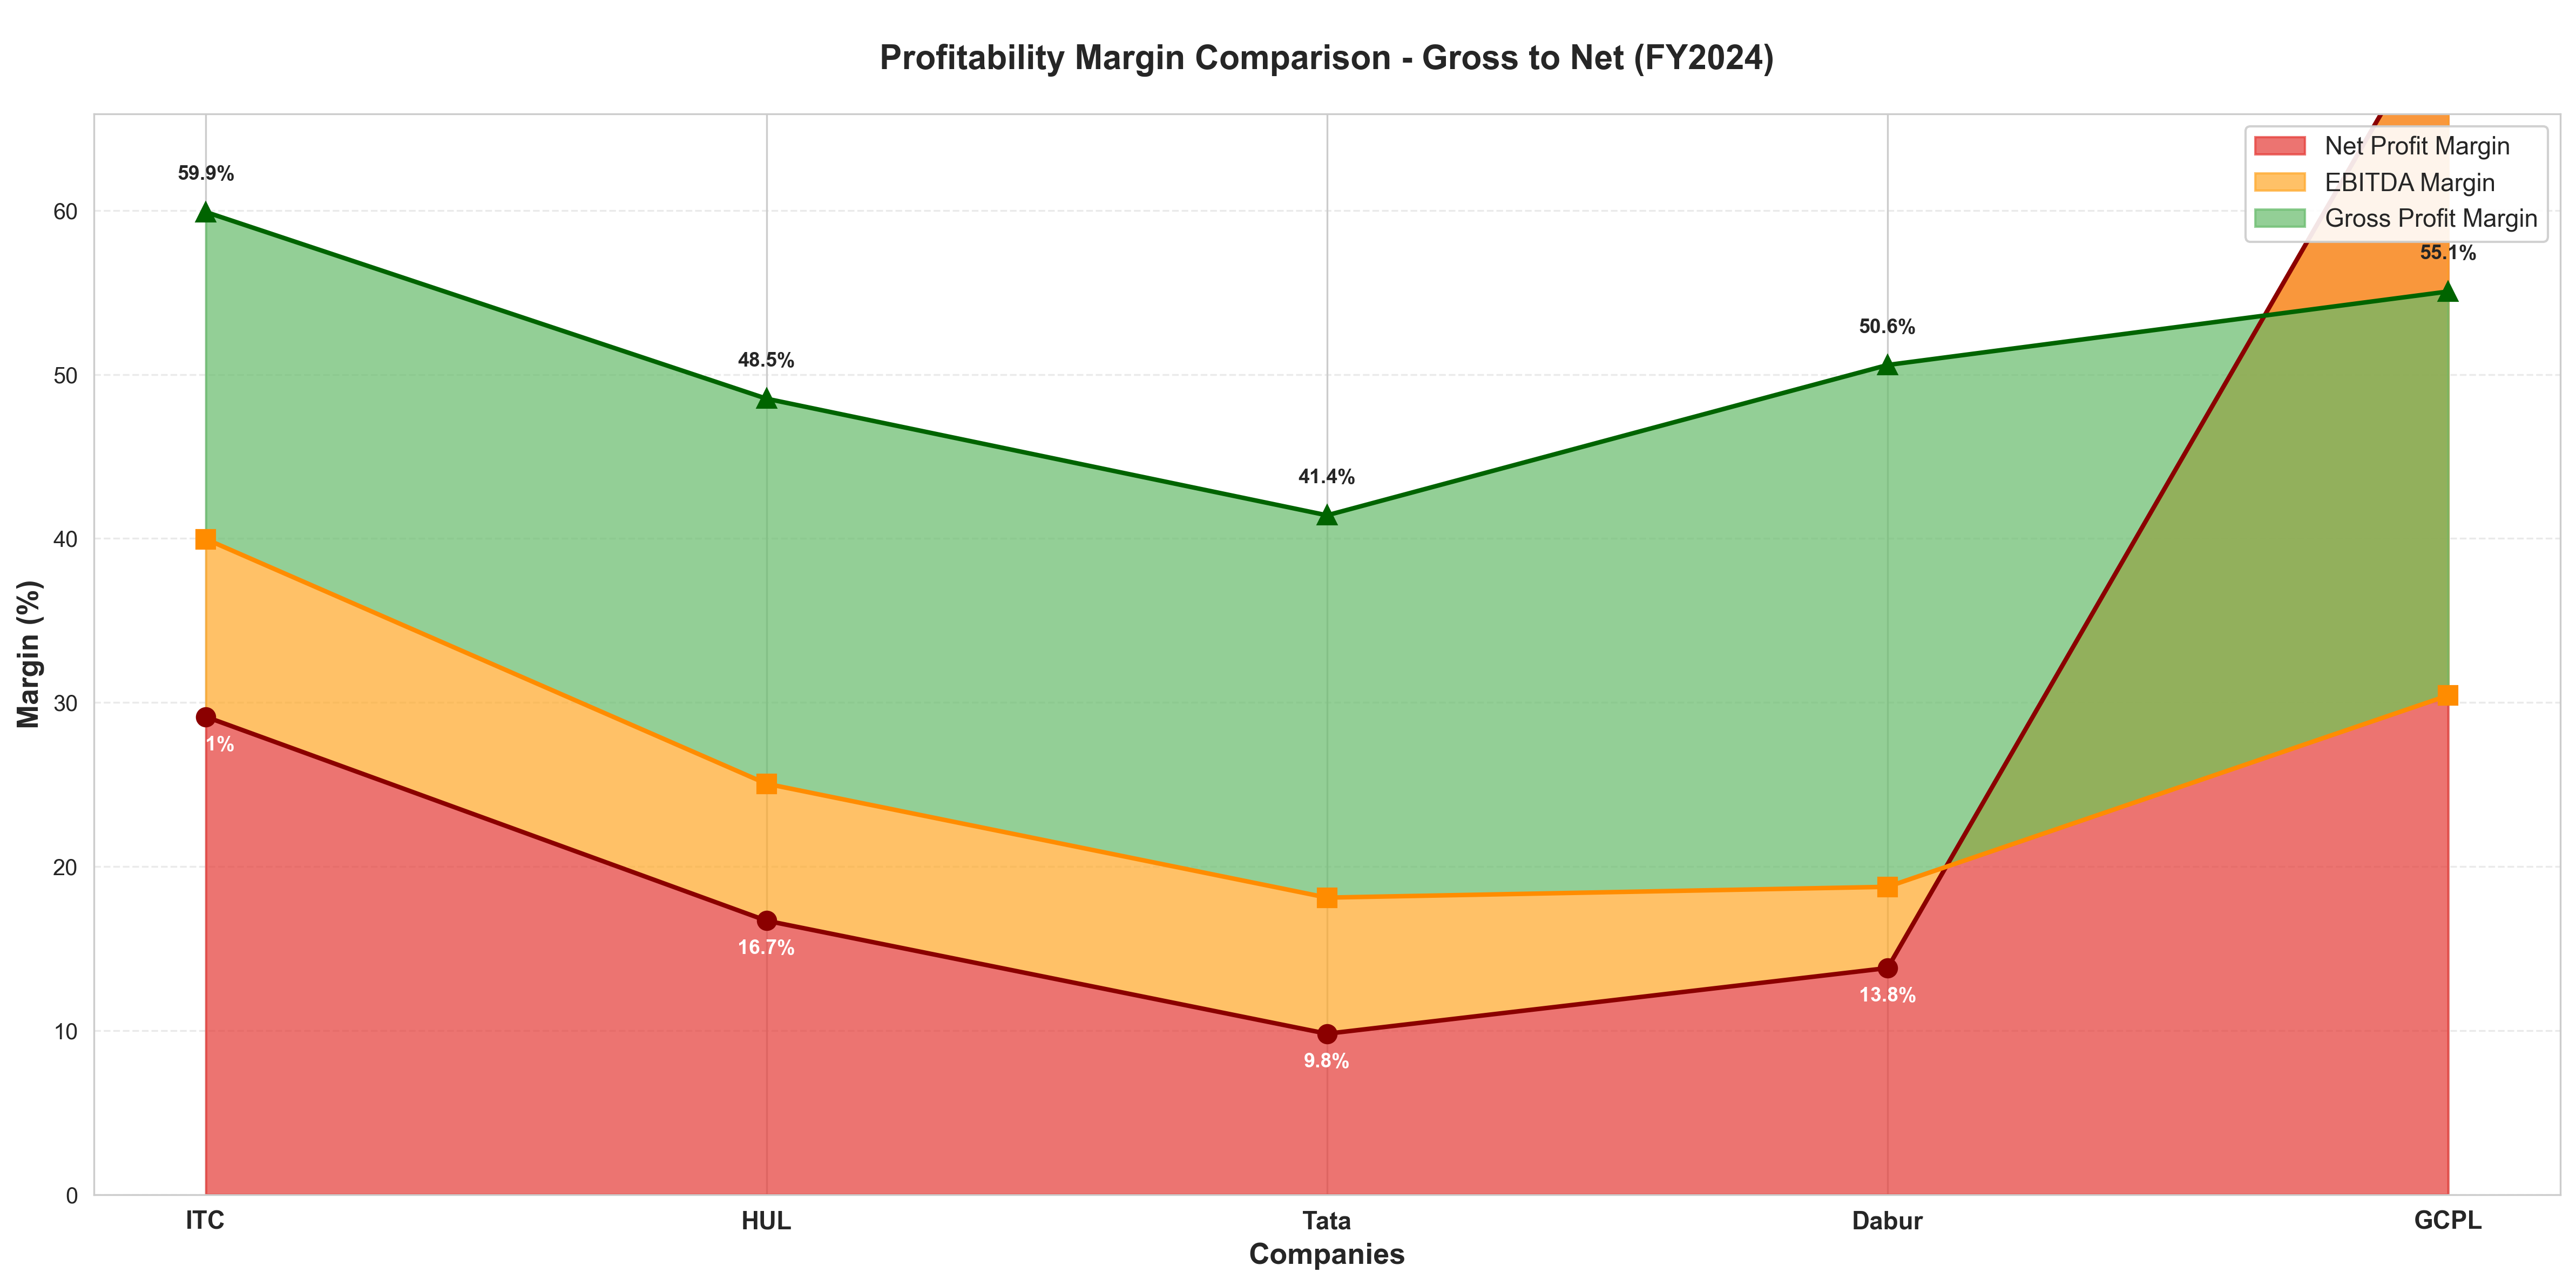
\includegraphics[width=0.8\textwidth]{assets/imperative_analysis/margin_comparison_area.png}
    \caption{Margin Comparison - Gross and Net Margins Across Companies}
\end{figure}

\vspace{0.3cm}

\section{Leverage Analysis: Capital Structure and Financial Risk}

\subsection{Conservative Capital Structures}

ITC maintains a pristine balance sheet with zero debt (D/E: 0.000), reflecting its strong cash generation capacity from tobacco operations. The reported 49.8\% leverage reduction appears to be a data artifact given the zero base.

Britannia executed significant deleveraging, halving its D/E ratio from 0.400 to 0.200 (50\% reduction). This strategic debt reduction, combined with declining profitability, suggests management prioritized financial stability over aggressive growth—a prudent choice for a food company facing volatile commodity markets.

Dabur maintained stable, moderate leverage (D/E: 0.328 → 0.343, +4.8\%), demonstrating disciplined capital allocation while funding operational improvements evidenced by its liquidity and profitability gains.

\subsection{Leverage Build-Up}

GCPL exhibited an astronomical 8,349\% increase in leverage, though the absolute D/E ratio remains conservative at 0.210 (starting from near-zero 0.002). This dramatic relative change likely reflects either debt-funded acquisitions, working capital financing, or capital structure optimization. When considered alongside the 70\% liquidity decline and 327\% profitability surge, this suggests a major corporate event—possibly an acquisition, restructuring, or strategic pivot.

HUL increased leverage 25.3\% (D/E: 0.424 → 0.531), likely reflecting working capital financing or dividend payments exceeding free cash flow. While the absolute ratio remains manageable, the upward trajectory warrants monitoring, especially given gross margin pressures.

Tata showed a modest 12.5\% leverage increase (D/E: 0.015 → 0.017), remaining negligible in absolute terms, suggesting its liquidity challenges stem from operational rather than financial leverage issues.

\begin{figure}[H]
    \centering
    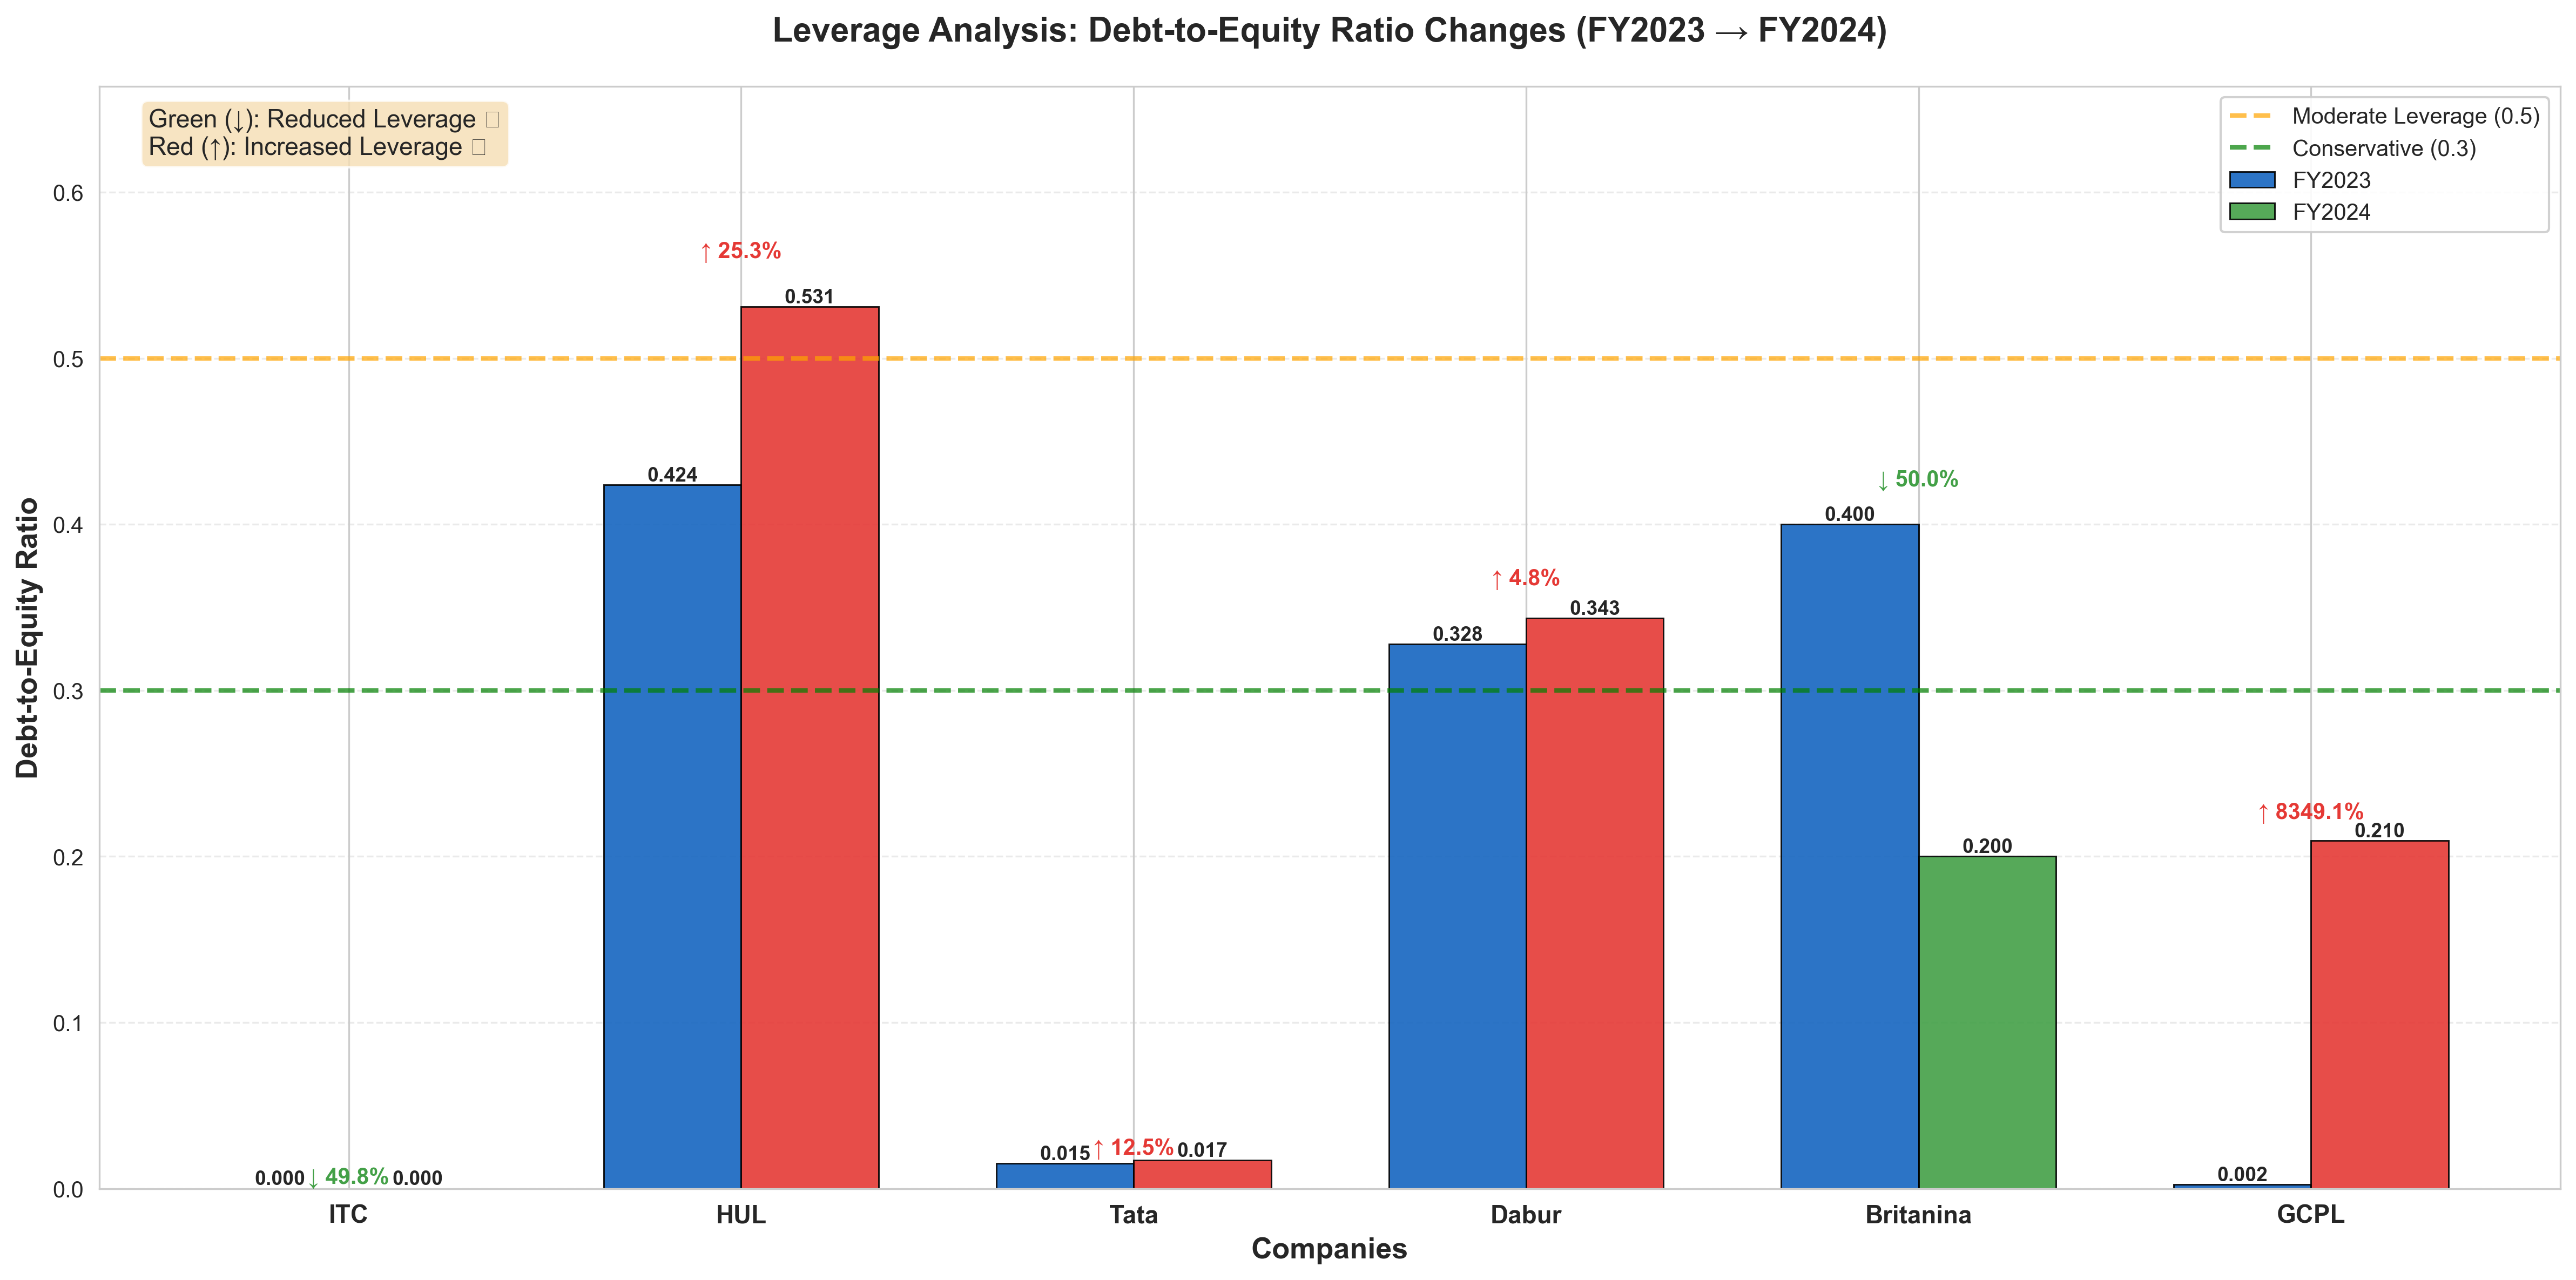
\includegraphics[width=0.8\textwidth]{assets/imperative_analysis/leverage_analysis.png}
    \caption{Leverage Analysis - Debt-to-Equity Ratios}
\end{figure}

\vspace{0.3cm}

\section{Operational Efficiency: Inventory Turnover Analysis}

\subsection{Efficiency Leaders}

Dabur improved inventory turnover 10\% to 5.17x, demonstrating the strongest operational efficiency gains. Combined with improved liquidity and profitability, this suggests comprehensive working capital optimization—faster production cycles, better demand forecasting, or strategic SKU rationalization.

Tata maintained stable, healthy inventory turnover at 3.88x (+0.6\%), indicating consistent operational performance despite profitability pressures and liquidity challenges. This stability suggests Tata's issues lie elsewhere in the working capital cycle, likely in receivables management or payables timing.

\newpage

% ===============================================
% CHAPTER 5: IMPERATIVE ANALYSIS
% ===============================================
\chapter{Imperative Analysis: Strategic Financial Imperatives}

\section{Framework and Methodology}

Imperative Analysis moves beyond standard financial metrics to identify and articulate the specific strategic priorities each company must execute to ensure sustainable value creation. Each company's analysis examines five critical imperatives: (i) Liquidity Management, (ii) Profitability Enhancement, (iii) Leverage Optimization, (iv) Operational Efficiency, and (v) Valuation Strategy. This framework identifies not merely what changed financially, but why it changed and what management must do to sustain positive trends or reverse concerning ones.

\section{Dabur India Limited}

\subsection{Executive Summary}

Dabur's FY24 financial performance demonstrates a company executing a disciplined operational turnaround while maintaining profitable growth. The critical imperatives center on sustaining liquidity improvements, leveraging margin gains for strategic reinvestment, and optimizing the capital structure to balance growth investments with shareholder returns.

\subsection{Liquidity Imperative: Consolidate and Leverage}

\subsubsection{Situation}
In FY24, Dabur witnessed a material improvement in its liquidity position, as evidenced by the rise in the Current Ratio from 0.85 to 1.19 and the Quick Ratio from 0.38 to 0.79. This transition indicates stronger short-term solvency, reflecting the company's enhanced capacity to meet its current obligations using its most liquid assets.

\subsubsection{Imperative Action}
The immediate opportunity is to consolidate these gains through disciplined working capital management. With improved liquidity now above unity, Dabur should: (i) institutionalize the processes that drove the 40\% current ratio improvement, (ii) establish target working capital days metrics to prevent regression, and (iii) deploy the freed-up cash strategically into growth initiatives rather than allowing it to accumulate as idle balances.

\subsubsection{Strategic Implication}
The higher ratios mitigate operational liquidity risk and better position Dabur to withstand unforeseen short-term financial stress. This financial flexibility enables the company to pursue organic expansion—capacity additions, new product launches, or geographic expansion—without the constraint of liquidity stress, contributing to both immediate operational resilience and long-term stability.

\subsection{Profitability Imperative: Sustain and Scale}

\subsubsection{Situation}
Dabur's profitability metrics show a notable uptrend. The Gross Profit Margin increased from 49.85\% to 50.58\%, and the Net Profit Margin improved from 11.96\% to 13.81\%. EBITDA margin also rose from 16.96\% to 18.76\%.

\subsubsection{Imperative Action}
These gains highlight improved pricing power, cost optimization efforts, and efficient management of input costs. To sustain this momentum, Dabur must: (i) protect pricing realizations through brand strengthening and premiumization of core portfolio, (ii) institutionalize cost savings rather than treating them as one-time wins, and (iii) invest margin gains into innovation and market-building to prevent competitor encroachment. Critically, the company should avoid the trap of allowing margin improvement to fund excessive SG\&A inflation or working capital deterioration.

\subsubsection{Strategic Implication}
The expansion in margins enhances short-term profitability, while sustained improvement supports organic growth potential and the reinvestment capacity necessary for long-term value creation. Each percentage point of margin improvement directly increases free cash flow available for dividends, debt reduction, or growth capex—expanding strategic optionality.

\subsection{Leverage Imperative: Maintain Conservative Structure}

\subsubsection{Situation}
The Debt to Equity Ratio increased slightly from 0.33 to 0.34, which indicates a marginal increment in leverage. Proprietary Ratio experienced a minor decline from 67.22\% to 65.66\%, but the Interest Coverage Ratio climbed from 75.62x to 85.89x, showing substantial improvement in the company's ability to service debt.

\subsubsection{Imperative Action}
These shifts demonstrate that management has consciously chosen to maintain conservative financial leverage. The key imperative is to preserve this fortress balance sheet by: (i) maintaining D/E ratios in the 0.30–0.40 range, (ii) using the exceptional interest coverage ratio as headroom for opportunistic debt-funded growth rather than perpetually deleveraging, and (iii) ensuring any incremental debt financing is deployed into return-generating investments (capex, acquisitions) rather than funding working capital or dividends.

\subsubsection{Strategic Implication}
These shifts suggest Dabur remains conservatively leveraged, maintaining low financial risk and strong solvency despite a marginal uptick in debt. Enhanced interest coverage further reduces financial distress risk, strengthening both short-term and long-term financing capacity and enabling the company to act decisively during sector downturns or M\&A opportunities.

\subsection{Operational Imperative: Accelerate Inventory Velocity}

\subsubsection{Situation}
Inventory Turnover ratio, which increased from 4.70x to 5.17x, reflects more efficient inventory management and faster conversion of inventory into sales. This operational efficiency boosts liquidity, minimizes holding costs, and reduces the risk of inventory obsolescence.

\subsubsection{Imperative Action}
Maintain and accelerate inventory velocity by: (i) strengthening demand sensing capabilities through enhanced retail data analytics and point-of-sale integration, (ii) implementing SKU rationalization to eliminate slow-moving variants, (iii) deepening vendor-managed inventory (VMI) programs with key retailers, and (iv) optimizing production batch sizes and scheduling to align supply with actual demand patterns rather than forecast bias.

\subsubsection{Strategic Implication}
The improvement supports a robust working capital cycle, strengthening liquidity and supporting cash flow stability vital for ongoing operations. Every incremental turn of inventory represents capital efficiently deployed, allowing the same balance sheet to support incrementally higher revenue and profit.

\subsection{Valuation Imperative: Recognize Earnings Growth}

\subsubsection{Situation}
Basic and Diluted EPS improved from ₹7.79 to ₹9.68, signaling robust earnings growth. However, the Price to Earnings (P/E) Ratio declined from 56.8x to 50.5x, suggesting either moderated investor expectations or relative undervaluation amidst earnings growth. The Dividend Payout Ratio fell from 70.6\% to 53.7\%, reflecting a policy shift toward earnings retention for growth initiatives.

\subsubsection{Imperative Action}
The declining P/E despite EPS growth presents a market efficiency opportunity. Management should: (i) communicate clearly to investors about the durability of margin improvements and their sources, (ii) articulate how retained earnings are being deployed (capex roadmap, M\&A pipeline, working capital optimization), (iii) consider selective buybacks during periods of P/E compression to return value while maintaining growth flexibility, and (iv) maintain consistent dividend policy signaling while retaining sufficient cash for strategic optionality.

\subsubsection{Strategic Implication}
Dividend Yield remained stable, aligning returns with market valuations and maintaining shareholder value. The 17\% payout ratio reduction creates a capital buffer for accelerating growth initiatives without dilutive equity raises, enabling Dabur to compound shareholder value through both earnings growth and strategic capital deployment.

\subsection{Strategic Alignment: DuPont Imperative}

\subsubsection{Situation}
The DuPont Margin ratio rose from 0.12 to 0.14, underscoring margin improvement's contribution to return on equity. The volume and leverage figures remain broadly stable year-on-year, indicating that higher profitability, rather than changes in asset utilization or leverage, drove the gains in ROE.

\subsubsection{Imperative Action}
This performance reveals that Dabur's superior profitability is the principal engine for value creation. Looking forward, the company should avoid the temptation to pursue ROE growth through increased leverage or aggressive asset expansion. Instead, the focus must remain on: (i) incremental margin accretion through pricing and cost discipline, (ii) modest asset turnover improvement through working capital optimization (as already achieved with inventory), and (iii) maintaining a conservative multiplier that preserves financial flexibility and risk mitigation.

\subsubsection{Strategic Implication}
This suggests Dabur's superior profitability is the principal engine for value creation, rather than riskier financial leverage or rapid asset turnover. A sustainable ROE trajectory depends on defending and expanding margins while avoiding the pitfall of margin exploitation that erodes brand equity or customer relationships.

\subsection{Key Imperatives Summary}

Dabur's financial turnaround positions it well for the next phase of sustainable growth. The imperatives center on three pillars: (i) \textbf{Consolidate liquidity gains} to enable strategic flexibility, (ii) \textbf{Sustain and scale profitability} through pricing discipline and cost institutionalization, and (iii) \textbf{Leverage conservative leverage} to fund growth without excessive financial risk. Success in executing these imperatives will determine whether the FY24 gains represent the start of a virtuous cycle or temporary wins that reverse under competitive or macro pressure.

\newpage

\section{ITC Limited}

\subsection{Executive Summary}

ITC's FY24 performance reveals a company navigating structural transitions in its legacy tobacco business while scaling new growth engines in FMCG, hotels, and agri-ventures. The financial profile—near-zero leverage, exceptional interest coverage, cash-rich balance sheet, and steady profitability—masks operational challenges requiring immediate strategic focus. The critical imperatives center on accelerating working capital optimization, protecting operating margins amid cost pressures, and deploying capital strategically toward high-return opportunities.

\subsection{Liquidity Imperative: Deploy Strategically Rather Than Hoard}

\subsubsection{Situation}
ITC's FY24 shows steady liquidity with Current Ratio improving slightly to approximately 3.0x while Quick Ratio was broadly steady, reflecting a cash-rich balance sheet and limited reliance on short-term debt despite ongoing investment across FMCG, hotels, and paperboards.

\subsubsection{Imperative Action}
ITC's exceptional 3.0x current ratio represents a fortress balance sheet but also signals potential inefficiency in capital deployment. The company should: (i) establish target liquidity ratios (e.g., 1.5–2.0x) and deploy excess cash into high-return, growth-oriented investments rather than maintaining exceptional cushions, (ii) accelerate capital deployment into identified growth opportunities—particularly in FMCG, where margins are improving and market position is strengthening, (iii) review and optimize the dividend vs. buyback mix to ensure capital is deployed to maximize per-share value creation rather than merely distributing excess liquidity, and (iv) consider strategic M\&A in adjacent high-growth segments where ITC's scale and distribution provide competitive advantage.

\subsubsection{Strategic Implication}
Stable operating cash generation and near-zero financial debt underpin short-term solvency; the small movements are mix effects rather than stress signals. Importantly, this stability should be leveraged as a strategic advantage—the confidence of suppliers, creditors, and investors in ITC's financial fortress provides optionality for bold strategic moves. The company that hesitates to deploy its balance sheet strength risks seeing markets reward more aggressive competitors.

\subsection{Profitability Imperative: Protect Margins While Driving Volume}

\subsubsection{Situation}
Gross and EBITDA margins rose as pricing, mix, and cost control offset a consumption slowdown in parts of FMCG. Management flagged resilient FMCG and record hotels performance in FY24, which supports the step-up at the operating line. Net margin increased on better operations and a slightly lower effective tax rate, though depreciation and investment for expansion tempered the upside.

\subsubsection{Imperative Action}
ITC achieved margin expansion despite mixed demand dynamics, reflecting strong operational execution. However, sustaining this requires: (i) pricing discipline grounded in value-add rather than mere cost pass-through—particularly critical as inflation moderates and pricing tolerance erodes, (ii) continuous focus on procurement and supply chain optimization to institutionalize cost savings, (iii) rigorous SKU rationalization in FMCG and paperboards to eliminate low-margin volume, concentrating scale on profitable segments, and (iv) leveraging improved hotels performance to drive higher-margin revenue mix across the portfolio.

\subsubsection{Strategic Implication}
The year ended with higher PAT on largely flat revenue, consistent with mix and efficiency gains. However, this ``margin without volume'' trajectory is structurally unsustainable—competitors are investing aggressively in capacity, and complacency risks market share loss. The imperative is to defend existing margins (through continuous improvement) while simultaneously pursuing volume growth in FMCG through innovation, geographic expansion, and e-commerce penetration.

\subsection{Leverage Imperative: Deploy Fortress Balance Sheet Prudently}

\subsubsection{Situation}
Debt-to-Equity is effectively nil and interest coverage is extraordinarily high, a consequence of strong internal accruals and minimal borrowings across segments, which lowers financial risk and preserves capacity for capex or buybacks/dividends as policy allows.

\subsubsection{Imperative Action}
ITC's near-zero leverage is a strategic asset, not a constraint. The company should: (i) maintain a disciplined but not excessive leverage position (D/E of 0.15–0.25 would be prudent), (ii) use modest leverage to fund high-ROIC investments rather than keeping the balance sheet perpetually fortress-like, (iii) ensure buybacks and special dividends are deployed only after securing funding for all organic capex and strategic investments, and (iv) consider strategic debt issuance if interest rates become favorable, using proceeds for acquisition or capex that exceeds available FCF—this preserves optionality and signals confidence to stakeholders.

\subsubsection{Strategic Implication}
With leverage already near zero, incremental ROE gains must come from margins and asset productivity rather than balance-sheet gearing, which frames capital allocation discussions for FY25. The imperative is clear: avoid the temptation of excess deleveraging, which would be financially inefficient, and instead deploy the balance sheet as a strategic weapon for growth and consolidation in attractive segments.

\subsection{Working Capital Imperative: Accelerate Inventory Velocity}

\subsubsection{Situation}
Inventory turnover slipped from approximately 3.21x to approximately 2.73x and stock velocity lengthened, indicating slower drawdown of stocks as paperboards/packaging faced a weaker cycle and FMCG demand decelerated in parts of the year, both of which reduce throughput per rupee of assets.

\subsubsection{Imperative Action}
The 15\% decline in inventory turnover is material and demands immediate action. ITC should: (i) conduct a detailed segment analysis to differentiate between cyclical (paperboards slowdown) and structural (FMCG demand deceleration) inventory buildup, (ii) implement aggressive inventory optimization programs for slower-moving SKUs, including promotional acceleration and potential SKU elimination, (iii) accelerate the deployment of demand-driven supply chain technologies (IoT tracking, predictive demand models) to reduce forecast bias and excess stock, (iv) strengthen retailer-level sell-through analytics and implement data-driven replenishment systems to align supply with actual demand, and (v) monitor whether paperboards inventory spike is cyclical (and will normalize as cycle recovers) or signals deeper demand weakness requiring capacity action.

\subsubsection{Strategic Implication}
External data also show inventory days rising into FY24–FY25, consistent with a longer cash conversion cycle until paperboards improve and FMCG volumes re-accelerate, making forecasting and SKU discipline key near-term levers. Critically, each day of excess inventory represents foregone cash flow and capital inefficiently deployed. Reducing inventory days even modestly (e.g., from 90 to 80 days) in a ₹50,000+ crore revenue company would unlock ₹5+ crore of cash.

\subsection{Market Value Imperative: Communicate Strategy Clearly}

\subsubsection{Situation}
EPS rose while P/E moved up modestly, implying investors paid a bit more for each rupee of earnings as the market priced steady cigarettes, hotels momentum, and FMCG margin traction despite mixed paper cycle signals. Dividend per share was moderated versus the prior year, lowering yield and normalizing the payout ratio.

\subsubsection{Imperative Action}
ITC's valuation trajectory (rising P/E) reflects investor recognition of operational progress despite structural headwinds. The company should: (i) clearly articulate the long-term vision for the conglomerate—is ITC a high-dividend, low-growth tobacco business in managed decline, or a diversified conglomerate transforming toward higher-growth FMCG/hotels/agri? This ambiguity creates valuation discounts, (ii) provide transparent segment ROE/ROIC disclosure to allow investors to value components and justify capital allocation to growth segments, (iii) establish clear capital allocation principles (e.g., organic capex first, then dividends, then M\&A) to reduce investor uncertainty, and (iv) signal dividend and buyback policy clearly—whether moderated payout ratios are temporary (to fund capex) or permanent (signaling mature business transition).

\subsubsection{Strategic Implication}
This preserves cash for growth and segment investments, a standard trade-off in ratio analysis when reinvestment opportunities are visible. However, the market is interpreting dividend moderation as either reluctance or opportunity for growth investment. Clarity on which is true could materially improve valuations and facilitate strategic capital raises if needed.

\subsection{Profitability Enhancement Imperative: DuPont Framework}

\subsubsection{Situation}
Using $\text{ROE} = \text{Net Margin} \times \text{Asset Turnover} \times \text{Equity Multiplier}$, FY24 shows higher margin, lower turnover, and a slightly lower multiplier, which together explain a broadly flat to marginally lower ROE, in line with the company-level ROE trend disclosed by third-party summaries.

\subsubsection{Imperative Action}
The DuPont decomposition reveals that margin improvement is being offset by turnover deterioration and multiplier compression. The strategic imperative requires managing all three levers: (i) keep margins firm by sustaining pricing discipline and cost control, particularly as cigarettes face tax headwinds and paperboards cycle down, (ii) re-accelerate turnover by fixing the inventory velocity problem described above and pursuing revenue growth through FMCG innovation and geographic expansion, and (iii) consider modest leverage increase (from near-zero base) to fund growth investments, thereby increasing the equity multiplier contributor to ROE.

\subsubsection{Strategic Implication}
The practical takeaway: to lift ROE, management must keep margins firm and re-accelerate turnover as demand normalizes and paperboards recover, since leverage is unlikely to be the chosen lever. This framework clarifies that ITC's near-term ROE trajectory depends critically on two factors: (1) defending FY24 margin gains despite moderating inflation reducing pricing tailwinds, and (2) reversing the inventory/turnover deterioration by accelerating volume growth. Without movement on both fronts, ROE risks heading lower despite ITC's strong balance sheet position.

\subsection{Key Operational Focus Areas}

\subsubsection{Working Capital Tightening}
Tighten working capital in FMCG and paperboards through sharper demand planning and SKU rationalization to bring inventory turns back toward FY23 levels and shorten stock days. This directly translates to cash liberation and improved ROIC.

\subsubsection{Operating Margin Protection}
Sustain pricing/mix and procurement benefits while hotels scale, keeping the EBITDA uplift intact through FY25 even if revenue growth is uneven by segment. Protect against cost inflation that could erode the margin gains.

\subsubsection{Capital Allocation Framework}
With negligible debt and high coverage, prioritize high-return capex in FMCG/packaging and calibrated dividends, using ROCE/ROE hurdles rather than leverage to drive per-share value. The fortress balance sheet should enable strategic optionality—bold investment in growth opportunities while maintaining shareholder returns.

\subsection{Key Imperatives Summary}

ITC stands at an inflection point. The company has successfully navigated FY24 with resilient operations, margin expansion, and strategic progress in growth segments (hotels, FMCG). However, the operational challenges—inventory slowdown, volume stagnation, mixed demand signals—demand immediate and sustained management focus. The imperatives are clear: (i) \textbf{Deploy capital strategically}, using the fortress balance sheet to fund growth in FMCG and adjacent high-return opportunities rather than hoarding liquidity, (ii) \textbf{Fix the working capital cycle} by accelerating inventory turnover and tightening receivables management, (iii) \textbf{Sustain margin expansion} through disciplined pricing and procurement while offsetting with volume growth from FMCG and hotels, and (iv) \textbf{Clarify the long-term conglomerate vision} to reduce valuation uncertainty and unlock investor appreciation of the transformation underway. Success in executing these imperatives will determine whether ITC emerges as a high-return growth compounder or experiences progressive margin compression and margin/valuation compression.

\newpage

\section{Britannia Industries}

\subsection{Executive Summary}

Britannia's FY24 performance reveals a company executing successful deleveraging and liquidity strengthening while simultaneously experiencing margin compression and deteriorating operational efficiency. The paradox of improving financial structure amid operational headwinds requires careful strategic navigation. The critical imperatives center on arresting the margin decline through operational excellence, restoring inventory efficiency to historical levels, and deploying improved leverage capacity strategically to fund growth initiatives that can reignite volume momentum.

\subsection{Liquidity Imperative: Strengthen But Monetize Position}

\subsubsection{Situation}
Britannia's liquidity position showed an improvement from FY23 to FY24. The Current Ratio increased from 1.03 to 1.17, and the Quick Ratio rose from 0.69 to 0.89. This indicates the company strengthened its short-term asset base relative to its current liabilities, enhancing its ability to meet immediate obligations.

\subsubsection{Imperative Action}
The 13.6\% improvement in current ratio, while positive, positions Britannia only marginally above the 1.0 minimum threshold and below the 1.5 industry comfort zone. The imperative is to: (i) ensure the liquidity improvement is durable by institutionalizing the working capital processes that drove it, rather than treating it as a temporary reprieve, (ii) avoid allowing improved liquidity to fund inefficient working capital practices or excessive inventory buildup (a concern given the inventory turnover collapse), (iii) deploy freed-up liquidity strategically toward growth capex or strategic initiatives rather than allowing it to accumulate as idle balances, and (iv) maintain sufficient liquidity buffers to weather potential demand shocks in a cost-conscious consumer environment.

\subsubsection{Strategic Implication}
The higher ratios suggest greater operational flexibility and a stronger buffer against liquidity shocks, supporting better short-term financial resilience and contributing positively to long-term financial stability. However, this financial stability must be leveraged to address the deeper operational challenges—margin compression and efficiency deterioration—rather than viewed as a satisfactory endpoint.

\subsection{Profitability Imperative: Arrest Margin Compression Urgently}

\subsubsection{Situation}
Profitability margins—gross, PBT, and net—declined in FY24 compared to FY23. The Gross Profit Margin fell slightly from 19.4\% to 18.9\%, the Net PBT Margin contracted from 18.6\% to 17.4\%, and the Net Profit Margin decreased from 14.2\% to 12.7\%. Returns on equity and assets also decreased, indicating a potential challenge in translating revenue growth into higher profits.

\subsubsection{Imperative Action}
The synchronized compression across gross, operating, and net margins—all declining simultaneously—signals systemic margin pressure rather than localized operational challenge. The imperative demands immediate, multi-pronged intervention: (i) \textbf{Gross margin stabilization}: conduct detailed input cost analysis to differentiate between unavoidable commodity inflation and controllable inefficiencies. Implement targeted pricing actions in premium segments (e.g., NutriChoice) where brand equity enables pricing power, while accepting mix shift toward more competitive value segments if necessary. Consider strategic SKU rationalization to eliminate products where input cost increases have eroded profitability below hurdle rates, (ii) \textbf{Operating expense discipline}: examine SG\&A inflation drivers—are distribution and marketing costs rising faster than revenue due to inefficient channels, excessive trade spend, or unproductive marketing spend? Implement zero-based budgeting for discretionary spend, (iii) \textbf{Mix management}: accelerate the shift toward higher-margin premium and wellness products where Britannia has competitive advantage and consumer willingness to pay. The 50+ basis point gross margin decline is concerning and suggests insufficient pricing realization or unfavorable mix shift toward lower-margin categories, and (iv) \textbf{Supply chain optimization}: invest in manufacturing efficiency, automation, and vendor consolidation to drive structural cost reduction independent of commodity cycles.

\subsubsection{Strategic Implication}
While Britannia remains profitable, these trends indicate margin pressure, which could dampen short-term profit generation and signal the need for strategic interventions to sustain long-term growth. Critically, margin compression compounds other challenges—lower profitability constrains cash generation for reinvestment, limits management's strategic flexibility, and erodes shareholder returns despite maintained dividend payout ratios. Without intervention, each further margin point of decline directly flows through to earnings and threatens the high dividend payout sustainability.

\subsection{Leverage Imperative: Deploy Improved Debt Capacity for Growth}

\subsubsection{Situation}
Britannia's leverage profile improved in FY24, as seen in the decline of the Debt to Equity Ratio from 0.4 to 0.2, suggesting a conscious shift toward lower reliance on debt financing. The Interest Coverage Ratio rose from 18.35 times to 21.69 times, indicating significantly enhanced ability to service debt from operative earnings.

\subsubsection{Imperative Action}
Britannia's successful 50\% deleveraging is strategically sound, but the risk now is under-utilizing this improved financial position. The imperative is to: (i) recognize that a 0.2 D/E ratio represents conservative leverage and provides substantial headroom for strategic debt-funded growth initiatives—the company should not pursue further deleveraging at the expense of forgoing growth opportunities, (ii) identify high-ROIC capital allocation opportunities: whether capacity expansion in core categories, premiumization of product lines, geographic expansion, or strategic acquisitions in adjacent categories (e.g., functional foods, plant-based proteins) where Britannia's brand equity and distribution can create value, (iii) evaluate whether modest leverage increase (to 0.35–0.40 D/E range) for growth capex would generate returns exceeding the cost of debt, thereby creating shareholder value, and (iv) ensure the improved interest coverage (21.69x) is viewed as capacity for strategic action, not justification for perpetual deleveraging that leaves the balance sheet under-optimized.

\subsubsection{Strategic Implication}
This improvement in financial risk positioning reduces vulnerability to changing interest rates and improves both short and long-term borrowing capacity. Importantly, Britannia now has strategic optionality available to most competitors—the ability to fund growth, defend market position against aggressive competitors, or execute strategic M\&A without equity dilution or financing stress. The imperative is to deploy this optionality before competitive dynamics shift or growth opportunities pass.

\subsection{Operational Efficiency Imperative: Restore Inventory Velocity}

\subsubsection{Situation}
Inventory turnover dropped sharply from 15.69 times in FY23 to 6.88 times in FY24. This dramatic 56.2\% decline is one of the most severe operational efficiency deteriorations across the FMCG peer set. This suggests inventory was held longer during FY24, potentially tying up more capital and possibly increasing carrying costs.

\subsubsection{Imperative Action}
The dramatic inventory turnover collapse demands urgent investigation and remediation. The imperative requires: (i) \textbf{Root cause analysis}: differentiate between cyclical factors (e.g., anticipated demand surge, seasonal stockpiling) and structural issues (demand forecasting failures, SKU over-production, retail channel destocking). Understanding causation is critical to prescribing appropriate response, (ii) \textbf{Demand sensing enhancement}: implement real-time point-of-sale data integration and retailer-level visibility to align production schedules with actual sell-through rather than forecast bias. Modern FMCG companies achieve this through advanced analytics and IoT integration—Britannia must modernize its demand planning infrastructure, (iii) \textbf{SKU rationalization}: the 56\% turnover decline suggests severe imbalance between production and demand. Immediate action should include aggressively eliminating slow-moving SKUs and reallocating production capacity toward core, fast-moving products, (iv) \textbf{Production flexibility}: evaluate whether manufacturing inflexibility (long lead times, minimum batch sizes) is forcing inventory buildup. Investing in flexible manufacturing (shorter changeover times, smaller economic batch sizes) could enable responsive supply management, and (v) \textbf{Promotional strategy}: accelerate movement of excess inventory through tactical promotions, trade schemes, and volume discounts—the cost of these actions is likely far lower than the cost of carrying inventory indefinitely.

\subsubsection{Strategic Implication}
The lower turnover may affect liquidity if not actively managed, although a still-moderate ratio indicates reasonable operational efficiency. However, this assessment understates the severity of the situation—the 56\% decline represents millions of rupees of working capital tied up inefficiently. If Britannia could restore inventory turns to FY23 levels (15.69x), it would liberate enormous cash currently trapped in slow-moving inventory, cash that could fund growth initiatives, reduce debt further, or enhance shareholder returns.

\subsection{Valuation Imperative: Communicate Path to Earnings Recovery}

\subsubsection{Situation}
Earnings per Share (EPS) declined marginally from ₹88.82 to ₹86.56, reflecting reduced net profitability despite overall earnings stability. The Price to Earnings (P/E) ratio remained constant at 66.30 times, signifying that investor expectations and market valuation remained robust, potentially due to Britannia's defensive sector positioning or expected recovery.

\subsubsection{Imperative Action}
The 66.3x P/E ratio is extraordinarily high—among the most premium valuations in the FMCG sector—and reflects market expectations for sustained high growth and profitability. This creates both opportunity and risk: (i) \textbf{communicate strategically}: use the market's confidence as a window to articulate a credible path to margin recovery and volume growth. The market is pricing in recovery; management must validate this optimism with concrete action plans, (ii) \textbf{execute visibly}: demonstrate progress on margin stabilization and inventory optimization through quarterly results and management commentary. Each quarter of execution builds valuation credibility; conversely, further deterioration could trigger a harsh re-rating, (iii) \textbf{shareholder return strategy}: the 83\% dividend payout ratio is sustainable only if profitability stabilizes. Management should signal whether dividend will be maintained at current absolute levels (risking compression of growth investment) or normalized to lower payout ratios to retain earnings for growth reinvestment. Clarity reduces valuation uncertainty, and (iv) \textbf{capital allocation transparency}: articulate how improved leverage capacity will be deployed—whether toward organic growth, M\&A, or further debt reduction. The market rewards clarity and coherent strategy.

\subsubsection{Strategic Implication}
The high Dividend Payout Ratio (over 83\% in both years) indicates a commitment to strong shareholder returns, though it implies limited profit retention for reinvestment. The tension between maintaining high dividends and funding growth investment is acute—if margins continue compressing and volume growth stalls, the dividend becomes unsustainable, risking a sharp correction in valuations and investor sentiment.

\subsection{ROE Imperative: Restore Volume as Primary Lever}

\subsubsection{Situation}
Return on Equity (ROE) decreased from 76.22\% in FY23 to 57.25\% in FY24, as derived from DuPont decomposition. Using $\text{ROE} = \text{Net Margin} \times \text{Asset Turnover} \times \text{Equity Multiplier}$, margin and leverage both improved (Margin from 12.7\% to 14.2\%, Leverage from 2.46 to 2.77), but despite rising leverage and margin, the reduction in volume (Asset Turnover) mitigated the benefits, leading to an overall lower ROE.

\subsubsection{Imperative Action}
The DuPont decomposition reveals the core strategic challenge: Britannia achieved margin improvement (paradoxically, given absolute margin compression mentioned earlier—this likely reflects lower depreciation or tax rate benefit) and increased leverage, but asset turnover collapsed, overwhelming these positive drivers. The imperative framework for ROE recovery is clear: (i) \textbf{Stabilize margins}: arrest the absolute margin compression through pricing, cost control, and mix management discussed above, (ii) \textbf{accelerate asset turnover}: this is the primary lever requiring immediate attention. Asset turnover collapsed because inventory turns plummeted. Restoring inventory efficiency from 6.88x toward 12-15x historical levels is non-discretionary—this directly translates to asset turnover improvement and ROE recovery, (iii) \textbf{leverage optimization}: maintain D/E in the 0.25–0.35 range; avoid excessive deleveraging that would reduce the multiplier benefit, and (iv) \textbf{volume growth}: ultimately, sustainable ROE recovery depends on translating margin stabilization and operational efficiency into revenue growth. Without volume growth, ROE gains are limited to working capital optimization (one-time benefit) and cannot compound.

\subsubsection{Strategic Implication}
Sustaining high ROE will require renewed focus on either improving margins or asset utilization. Given the margin pressures already evident, the near-term imperative centers on asset utilization—specifically, fixing the inventory turnover catastrophe. Success here would immediately improve ROE. Over the medium term, however, volume growth is essential; margin stabilization alone is insufficient for sustainable ROE recovery.

\subsection{Key Imperatives Summary}

Britannia stands at a critical juncture. The company has successfully deleveraged and improved its liquidity position, earning financial flexibility. However, this structural improvement in balance sheet strength is being offset by deteriorating operational metrics—margin compression, inventory efficiency collapse, and ROE decline. The window to deploy improved financial capacity toward growth initiatives is narrowing; further quarters of operational deterioration could trigger valuation compression that erodes the confidence enabling current leverage-funded investment.

The imperatives are urgent and specific: (i) \textbf{Arrest margin compression} through pricing discipline in premium segments, cost structure optimization, and product mix management—this is existential as compressed margins constrain cash generation and dividend sustainability, (ii) \textbf{Restore inventory efficiency} through demand sensing modernization, SKU rationalization, and inventory acceleration—this is the fastest lever to improve working capital and operational ROE, (iii) \textbf{Deploy improved leverage capacity strategically} toward growth capex or high-ROIC opportunities that can reignite volume momentum—the balance sheet improvement is valuable only if deployed, not if hoarded, and (iv) \textbf{Communicate credibly to the market} a path to earnings recovery and capital allocation strategy—the 66.3x P/E valuation provides limited margin of safety and is vulnerable to negative surprises. Transparency and execution are essential to maintain investor confidence and prevent re-rating.

Success in executing these imperatives will determine whether Britannia remains a defensive sector stalwart commanding premium valuations, or experiences a slide into margin compression, valuation pressure, and shareholder value destruction characteristic of companies unable to navigate margin cycles.

\newpage

\section{Hindustan Unilever Limited (HUL)}

\subsection{Executive Summary}

HUL's FY24 performance reveals a company executing a deliberate strategic pivot: sacrificing short-term gross margin to defend volume, investing aggressively in brand-building and distribution to maintain market leadership, and managing a complex balance sheet featuring significant capex and lease-related financial liabilities. The financial profile—improved liquidity, stable net profitability, and elevated dividend payout—masks underlying operational tensions: margin give-backs, inflationary cost pressures, and SKU complexity driving inventory efficiency challenges. The critical imperatives center on rationalizing the product portfolio to improve margin quality, accelerating cash conversion through working capital optimization, and justifying the aggressive cost-of-sales and SG\&A investments through demonstrated volume recovery.

\subsection{Liquidity Imperative: Leverage Improved Position for Strategic Action}

\subsubsection{Situation}
Current ratio improved to approximately 1.64x from approximately 1.38x and quick ratio to approximately 1.33x from approximately 1.03x, driven by a sharp rise in current assets (₹20,296 cr in FY24 vs ₹16,049 cr in FY23) against a milder rise in current liabilities (₹12,403 cr vs ₹11,627 cr), giving the business more room to fund day-to-day operations from its own working capital cycle. Inside the working-capital mix, trade receivables and cash were healthy while payables also rose, which together suggests stronger channel activity and disciplined payables management rather than distress-driven borrowing.

\subsubsection{Imperative Action}
HUL's 19\% improvement in current ratio and 29\% improvement in quick ratio demonstrate successful working capital management and operational cash generation. The imperative is to: (i) sustain the working capital discipline that enabled this improvement—particularly the balanced growth in payables, which suggests strong vendor relationships and favorable payment terms rather than creditor pressure, (ii) deploy the freed-up liquidity strategically toward high-ROI opportunities: whether accelerated innovation in high-growth categories, expansion into emerging segments (e.g., premium naturals, functional foods), or geographic expansion into underpenetrated regions, (iii) maintain current ratio in the 1.5-1.8x range, recognizing that ratios above 1.8x represent excess liquidity that could be deployed more productively, and (iv) avoid allowing improved liquidity to fund margin-destructive promotional spending or inefficient SKU proliferation—the working capital improvement should enable growth investment, not working capital degradation.

\subsubsection{Strategic Implication}
The improved liquidity provides operational flexibility and reduces short-term financial stress, positioning HUL to pursue organic growth initiatives, seasonal working capital needs, and opportunistic investments without liquidity constraints. However, this financial flexibility is valuable only if deployed toward value-creating initiatives; hoarding liquidity wastes shareholder capital.

\subsection{Profitability Imperative: Stabilize Margin Trajectory Through SKU Discipline}

\subsubsection{Situation}
Gross margin printed lower (48.5\% vs 52.8\%) even as cost of materials fell year-on-year (₹17,791 cr vs ₹19,229 cr), pointing to price rollbacks/grammage restoration in select categories and a higher share of traded goods that compress accounting gross margin despite input deflation. EBITDA margin rose to approximately 25.1\% from approximately 24.0\% as operating efficiencies and savings offset the gross margin give-back, while ``other expenses'' climbed (₹14,170 cr vs ₹11,703 cr), consistent with stepped-up brand building, distribution, and go-to-market spending.

\subsubsection{Imperative Action}
The 430 basis point gross margin decline despite falling input costs is striking and signals a deliberate strategic choice: HUL sacrificed margin to defend/grow volumes through pricing restraint and grammage restoration. This is a high-risk strategy that requires disciplined execution: (i) \textbf{Justify the margin sacrifice through volume}: the imperative is to demonstrate that volume growth, market share gains, or category expansion justify the margin compression. If volume growth disappoints, the margin sacrifice becomes indefensible, (ii) \textbf{manage the SKU complexity}: the mention of ``higher share of traded goods'' and ``richer SKU mix'' suggests portfolio proliferation. HUL must rationalize SKUs to focus on high-margin products and eliminate low-margin traded goods that compress overall gross margin without proportional volume benefit, (iii) \textbf{control SG\&A inflation}: while brand-building spending is defensible if it drives profitable growth, the ₹2.5 crore increase in other expenses must translate into demonstrable ROI through market share gains or volume acceleration. Establish clear ROI hurdles and hold marketing/distribution spend accountable to measurable outcomes, and (iv) \textbf{stabilize net margin}: HUL has successfully held net margin flat despite gross margin compression, demonstrating operational excellence. This cannot be sustained indefinitely—if gross margins compress further without operating leverage benefit, net margins will eventually deteriorate.

\subsubsection{Strategic Implication}
PAT grew (₹10,098 cr vs ₹9,856 cr) and net margin was broadly flat (approximately 16.7\% vs approximately 16.7\%), meaning operating execution and scale gains absorbed the higher below-the-line costs and kept bottom-line quality intact. However, this stable net margin amid gross margin compression reflects disciplined cost management that cannot be perpetually maintained—each additional basis point of gross margin compression flows through with mathematical certainty to net margin unless offset by equivalent operating expense reductions.

\subsection{Leverage Imperative: Manage Balance Sheet Complexity Strategically}

\subsubsection{Situation}
Debt-to-equity rose (≈0.53x vs ≈0.42x) and interest coverage fell sharply (≈46x vs ≈129x) because finance cost moved up materially (₹302 cr vs ₹101 cr), reflecting higher lease/financial liabilities and a larger asset base, not weakening operations. Non-current liabilities increased (₹13,700 cr vs ₹9,977 cr) while PPE grew (₹7,178 cr vs ₹6,189 cr), indicating investment and financing choices that lift capacity and capability but add interest and depreciation in the near term.

\subsubsection{Imperative Action}
The 26\% increase in D/E and dramatic interest coverage decline (from 129x to 46x) warrant careful analysis. While the absolute interest coverage remains robust at 46x, the trajectory is concerning if it reflects increased leverage rather than one-time capex financing. The imperative is to: (i) \textbf{justify the capex decisions}: the ₹989 cr increase in PPE represents significant capital deployment. Management must articulate the ROIC of these investments and the timeline to payback—whether capacity expansion, automation, or facility upgrades, (ii) \textbf{manage lease liabilities carefully}: the increase in finance costs driven by lease obligations (under IFRS 16 / IndAS 116) suggests expanded retail footprint or supply chain facilities. While lease financing is economically rational, ensure the decisions are based on strategic necessity rather than opportunistic expansion that could become stranded if consumer demand shifts, (iii) \textbf{avoid further leverage escalation}: maintain D/E in the 0.45–0.55 range; beyond this level, leverage becomes constraining for strategic optionality and dividend capacity. The 0.53 level is acceptable but represents an upper bound, not permission for further increases, and (iv) \textbf{prioritize debt reduction as earnings improve}: as input deflation moderates and pricing normalizes, leverage should trend downward. Use earnings growth not for dividend increases but for debt paydown until D/E returns to historical 0.35–0.40 levels.

\subsubsection{Strategic Implication}
Interest coverage fell from an extraordinary 129x to 46x due to increased financial liabilities and depreciation. While 46x coverage is exceptional by any standard and poses zero financial risk, the trajectory must be monitored. If coverage declines below 25x or leverage rises above 0.65x D/E, financial flexibility constraints could limit strategic optionality during downturns or M\&A opportunities.

\subsection{Working Capital Imperative: Rationalize SKU Mix and Accelerate Turnover}

\subsubsection{Situation}
Inventory turnover reported at approximately 7.48x implies days-on-hand of about 49 days, while stock velocity at approximately 3.92x signals slower drawdown versus sales intensity, a pattern consistent with a tougher consumer backdrop and a richer SKU mix in staples and BPC (Beauty \& Personal Care). The balance sheet shows inventories higher year-on-year within growing current assets, so cash conversion will benefit from tighter forecasting and SKU discipline as demand normalizes.

\subsubsection{Imperative Action}
HUL's inventory profile reveals operational complexity requiring immediate attention: (i) \textbf{SKU rationalization}: the mention of ``richer SKU mix'' is code for portfolio proliferation. While assortment expansion is sometimes defensible (e.g., premiumization, segment-specific products), it often results in inventory fragmentation, lower turnover, and excessive capital lock-up. HUL should conduct a ruthless SKU review: eliminate low-velocity variants, consolidate packaging options, and concentrate production and marketing on core, fast-moving products. This alone could improve inventory turns and free significant working capital, (ii) \textbf{demand sensing modernization}: implement real-time POS data integration and AI-driven demand forecasting to reduce forecast bias. HUL's scale enables investment in advanced analytics that many competitors cannot justify—this is a competitive advantage that must be deployed, (iii) \textbf{inventory optimization by channel}: different channels (e.g., kirana, modern trade, e-commerce) have different SKU velocity and working capital implications. Optimize inventory positioning by channel to maximize turnover, and (iv) \textbf{promotional discipline}: the aggressive promotional spending (reflected in SG\&A) may be driving inventory build if promotions are forward-shifting demand. Implement ROI-based promotional planning to ensure each promotional event drives profitable incremental volume rather than merely shifting demand forward and inflating inventory.

\subsubsection{Strategic Implication}
While 7.48x inventory turnover is healthy in absolute terms, the 49-day inventory cycle ties up substantial working capital. Every percentage point improvement in inventory turns translates to significant cash liberation—in HUL's revenue base of ₹50,000+ cr, a 10\% improvement in inventory efficiency would free ₹500+ cr of cash that could fund growth, reduce debt, or enhance shareholder returns.

\subsection{Valuation Imperative: Justify Premium Valuation Through Visible Growth}

\subsubsection{Situation}
EPS was broadly stable into FY24, while valuation multiples were elevated (P/E ~59.4x vs ~54.7x) and the dividend payout ratio remained high (~96\% vs ~91\%), implying the market paid up for the franchise's consistency and cash return even as management kept reinvesting in brands and capacity. Dividend per share rose (₹42 vs ₹39) with yield steady near 1.8\%.

\subsubsection{Imperative Action}
HUL's 59.4x P/E represents one of the highest valuations in the FMCG sector, reflecting investor faith in the company's brand equity, distribution dominance, and dividend stability. However, this premium valuation is vulnerable to negative surprises and requires careful management: (i) \textbf{deliver visible earnings growth}: EPS stability in FY24 is acceptable for a mature company but insufficient to justify further multiple expansion. HUL must demonstrate EPS growth of 8-10\%+ annually to justify the premium valuation. Growth must come from volume expansion (not just inflation passthrough) or margin recovery as input costs normalize, (ii) \textbf{signal dividend policy clearly}: the 96\% payout ratio is extraordinarily high and leaves minimal room for earnings volatility or capex surprises without cutting dividends. Management should signal whether the payout ratio will normalize to 70-75\% to provide earnings buffer, or whether dividends will be maintained at absolute levels while payout ratio compresses as earnings grow, (iii) \textbf{communicate capex ROI}: the significant capex and lease financing in FY24 must be justified through ROI analysis. Transparent communication about expected returns from these investments would improve investor confidence and support valuations even amid near-term margin pressures, and (iv) \textbf{manage market expectations carefully}: with such elevated valuations, any quarter of disappointing results could trigger sharp re-rating. Conservative guidance and under-promise/over-deliver execution is prudent.

\subsubsection{Strategic Implication}
Dividend per share rose (₹42 vs ₹39) with yield steady near 1.8\%, which is coherent with a high-payout, low-net-debt profile and sustained free-cash generation. The 96\% payout ratio reflects confidence in earnings quality and cash flow stability, but leaves no margin for error if profitability comes under pressure. If margin compression continues or volume growth disappoints, dividend sustainability becomes questionable, risking a harsh re-rating.

\subsection{Strategic Positioning Imperative: Navigate Volume vs. Margin Trade-Off}

\subsubsection{Situation}
HUL's FY24 strategy reflects a deliberate choice: sacrifice gross margin (through pricing restraint and grammage restoration) to defend volume and market share, while investing aggressively in brand-building and distribution (SG\&A up 21\%) to drive category penetration and consumer engagement. This is fundamentally different from peers like Dabur (pursuing margin expansion) or ITC (balancing margin and volume).

\subsubsection{Imperative Action}
This strategic positioning is defensible but requires perfect execution. The imperative is to: (i) \textbf{ensure volume growth materializes}: the margin sacrifice is justified only if it delivers volume growth exceeding inflation. If volumes are flat or declining despite the margin sacrifice, the strategy has failed and management must course-correct immediately, (ii) \textbf{establish clear exit criteria}: define the conditions under which HUL would reverse the volume-focused strategy and return to margin expansion. This prevents perpetual margin erosion if volume growth disappoints, (iii) \textbf{leverage scale advantages}: HUL's distribution and brand scale should enable it to navigate margin cycles better than smaller competitors. Use this advantage to gain market share during constrained periods and extract pricing power during recovery, and (iv) \textbf{pursue premiumization in parallel}: while defending volume in core categories, simultaneously build premium sub-brands and adjacent categories (e.g., naturals, functional products) where higher margins are achievable. This dual-track strategy balances volume defense with margin enhancement.

\subsubsection{Strategic Implication}
HUL is betting that aggressive volume defense and market share gains in FY24 will position it for margin recovery as: (i) input costs normalize and inflation moderates, (ii) consumer demand rebounds and pricing power returns, and (iii) brand investments drive trading-up and category expansion. This bet is reasonable but contingent on execution across multiple fronts. If any link breaks, profitability could deteriorate sharply.

\subsection{Key Imperatives Summary}

HUL stands at a critical inflection point between two strategic paths. The company is choosing to prioritize volume defense and market share through aggressive investment (SG\&A up 21\%, capex expansion, lease financing) while sacrificing gross margin. This is a high-conviction bet that improved market position will enable margin recovery and earnings reacceleration once input cost inflation moderates and demand normalizes.

The imperatives are clear and contingent on successful execution: (i) \textbf{demonstrate volume growth} to justify the margin sacrifice—if volumes remain flat despite aggressive investments, the strategy fails and must be reversed, (ii) \textbf{rationalize SKU portfolio} to improve inventory efficiency and reduce working capital drag—every point of inventory turn improvement liberates cash for reinvestment, (iii) \textbf{manage leverage prudently} by containing D/E in the 0.45–0.55 range and prioritizing debt reduction as margins recover—avoid the trap of perpetual leverage escalation, (iv) \textbf{justify premium valuation} through visible earnings growth and transparent ROI communication on capex and brand investments, and (v) \textbf{prepare for margin recovery} by defining clear trigger points for pricing actions and capacity investments—once consumer demand normalizes and input cost inflation moderates, HUL must execute disciplined pricing to recover margin.

Success in executing these imperatives will determine whether HUL emerges from this investment phase with enhanced market position and earnings momentum, or finds itself trapped in a structural margin compression cycle unable to recover pricing power despite having sacrificed profitability to defend volume. The market is paying a premium valuation for HUL's franchise strength; management must justify this premium through visible delivery of profitable growth.

\newpage

\section{Comparative Rankings and Strategic Positioning}

\subsection{Efficiency Concerns}

Britannia suffered a dramatic 56.2\% inventory turnover collapse from 15.69x to 6.88x. This severe deterioration, while still above the 5x efficiency threshold, signals potential issues: demand forecasting failures, production over-scheduling, or raw material stockpiling ahead of anticipated price increases. Combined with declining profitability and improving liquidity, this suggests Britannia converted cash into inventory—potentially tying up working capital inefficiently.

ITC experienced a 15.2\% inventory turnover decline to 2.73x, indicating slower stock conversion. For a diversified conglomerate, this could reflect strategic inventory building in hotels (ahead of seasonal demand) or FMCG (anticipating supply chain disruptions), but nevertheless represents capital tied up earning suboptimal returns.

HUL and GCPL lack reported inventory turnover data, preventing comprehensive operational efficiency assessment.

\begin{figure}[H]
    \centering
    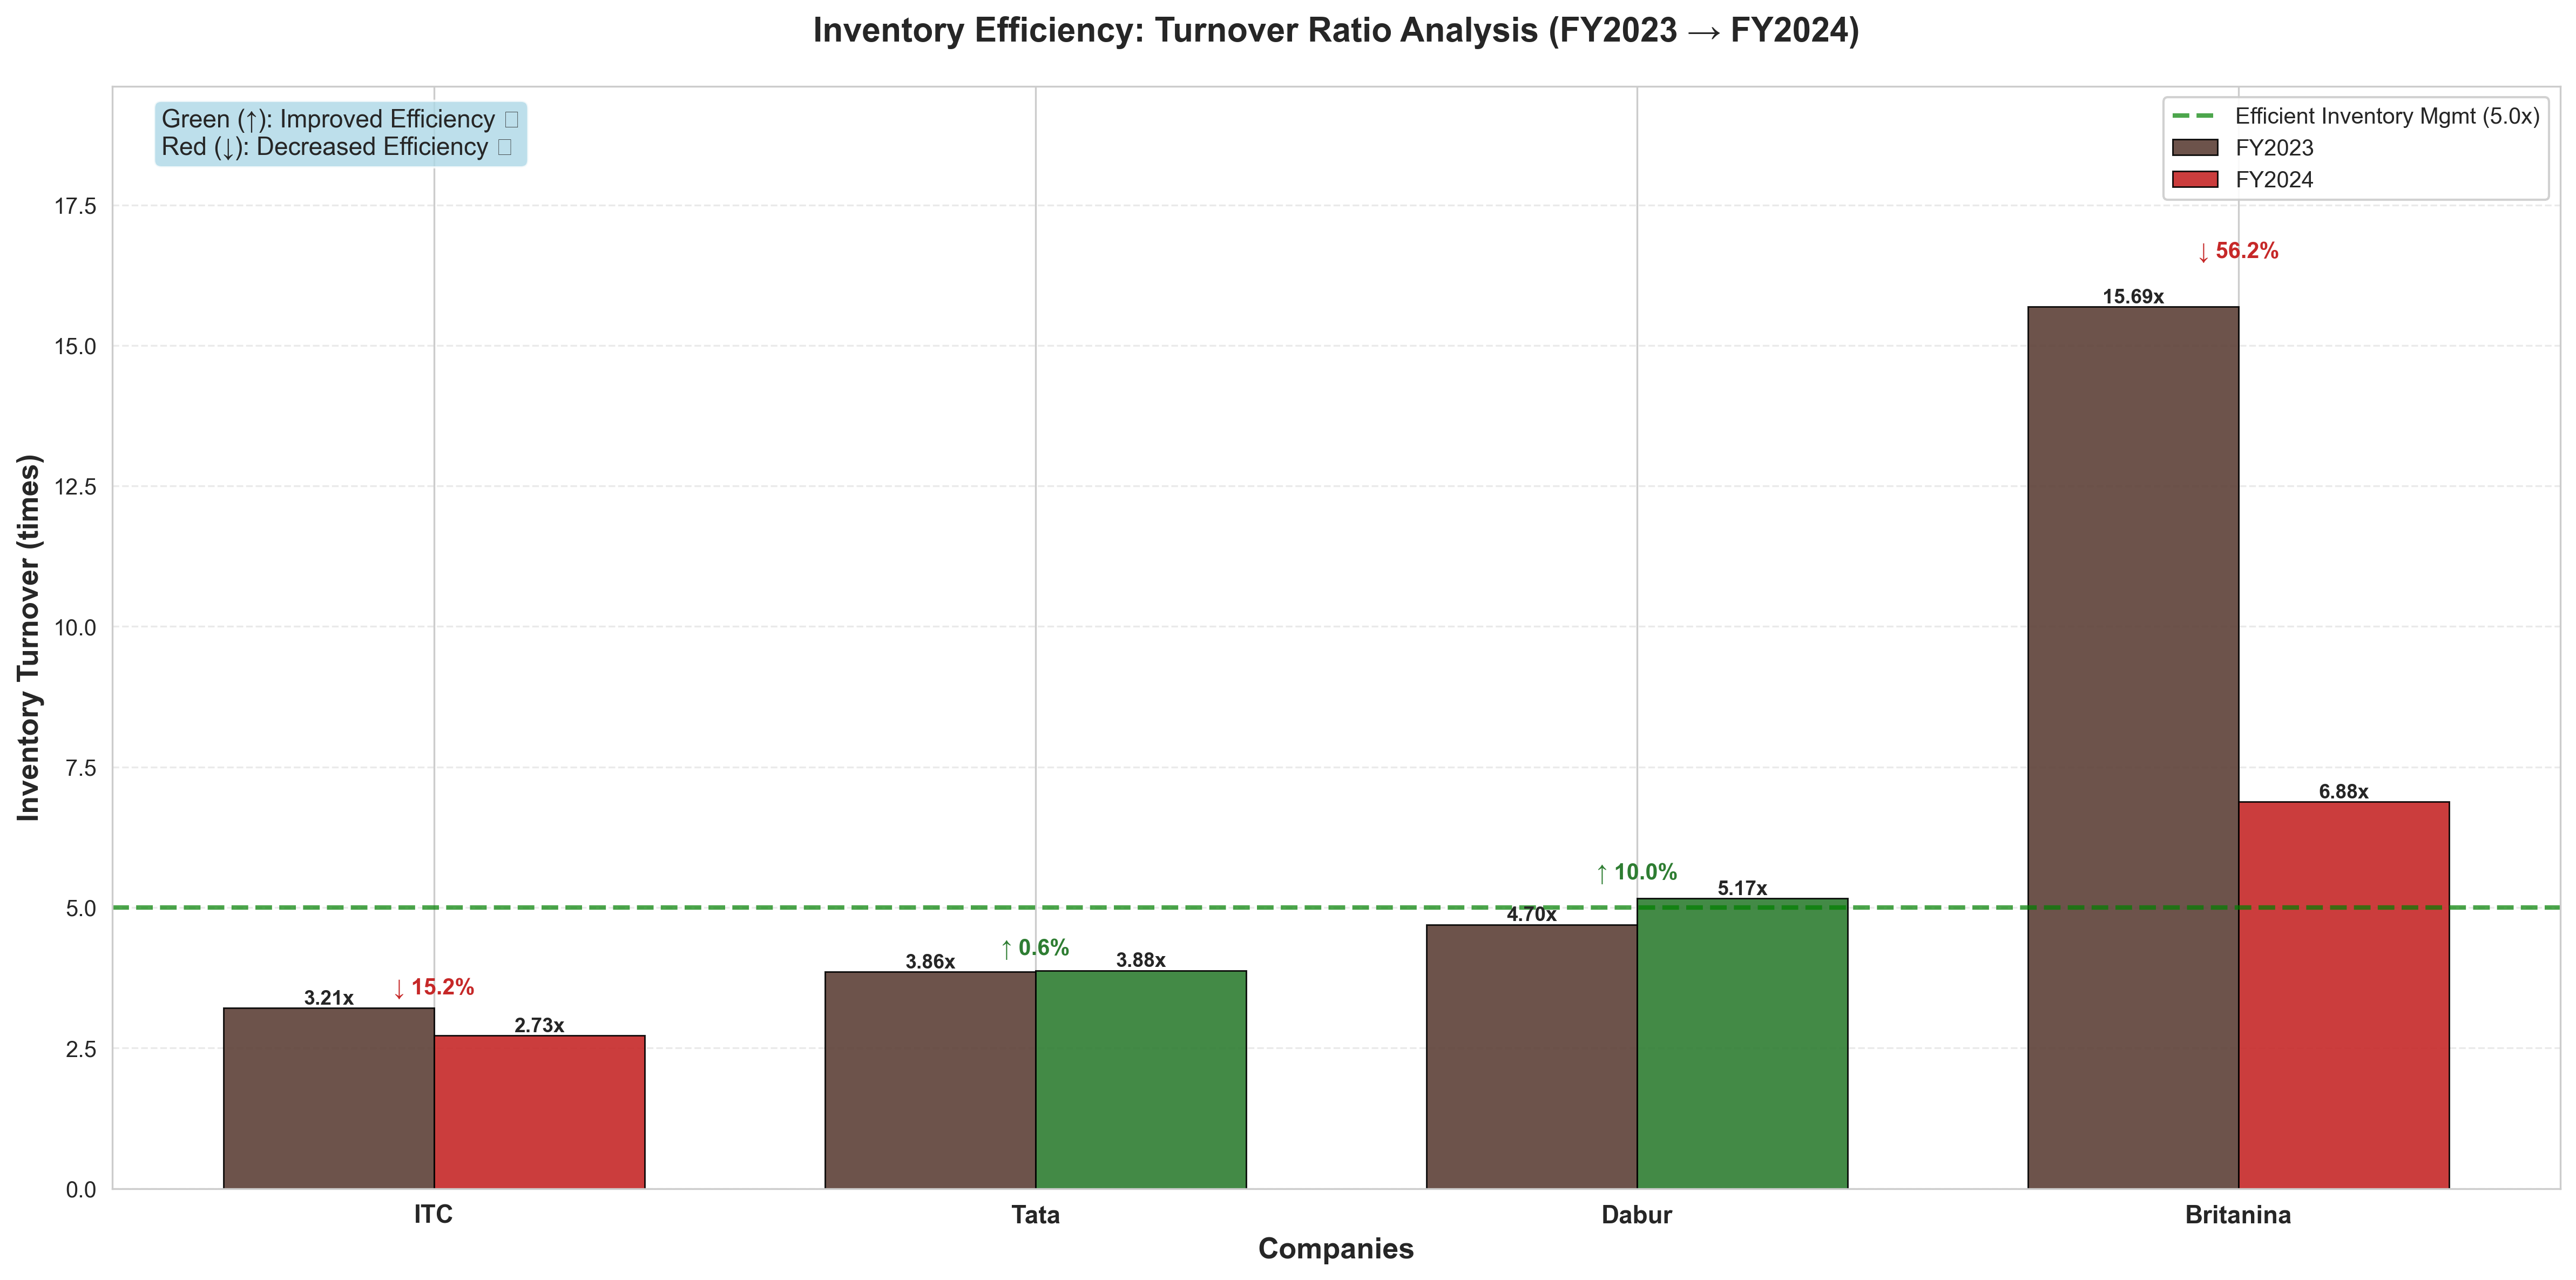
\includegraphics[width=0.8\textwidth]{assets/imperative_analysis/inventory_analysis.png}
    \caption{Inventory Analysis - Turnover Ratios}
\end{figure}

\vspace{0.3cm}

\section{Comparative Rankings and Strategic Positioning}

\subsection{Overall Financial Health Leaders}

\begin{itemize}
    \item \textbf{ITC:} Excellent liquidity (2.91), exceptional profitability (29.1\%), zero debt, though inventory efficiency declined
    \item \textbf{Dabur:} Balanced improvement across all metrics—40\% liquidity gain, 15.5\% profitability increase, 10\% efficiency improvement
    \item \textbf{HUL:} Solid liquidity recovery (18.6\%), stable profitability amid margin pressures, moderate leverage increase
\end{itemize}

\subsection{Companies Requiring Strategic Review}

\begin{itemize}
    \item \textbf{GCPL:} Extreme volatility across all metrics suggests major corporate event requiring investigation
    \item \textbf{Tata:} Severe liquidity crisis (-66\%) despite minimal leverage and stable inventory turnover
    \item \textbf{Britannia:} Profitability and efficiency deterioration despite successful deleveraging
\end{itemize}

\section{Strategic Implications and Recommendations}

\subsection{For Strong Performers (ITC, Dabur)}

These companies should leverage their financial strength for strategic initiatives: market share gains through competitive pricing, strategic acquisitions, or capacity expansion. ITC's inventory slowdown requires attention to ensure working capital efficiency isn't deteriorating.

\subsection{For Companies Under Pressure (Tata, Britannia)}

Immediate focus should address liquidity challenges through accelerated receivables collection, inventory optimization, and potentially renegotiating payment terms with suppliers. The profitability pressures require detailed cost structure analysis to identify controllable expense reduction opportunities.

\subsection{For GCPL}

The extreme metric volatility demands transparent disclosure about the underlying drivers—whether M\&A activity, restructuring, or one-time events. Until clarity emerges, the sustainability of the 73\% net margin and implications of the liquidity collapse remain uncertain.

\subsection{For HUL}

While maintaining stable profitability despite gross margin compression demonstrates operational discipline, this strategy is unsustainable long-term. Management must address the underlying gross margin pressures through innovation, premiumization, or supply chain optimization rather than perpetually squeezing operating expenses.

\section{Conclusion}

The FMCG sector demonstrates bifurcated performance: established leaders like ITC and improving players like Dabur strengthened their competitive positions through balanced financial management, while others face operational challenges or underwent transformative events. The sector appears to be navigating input cost inflation with varying success, with profitability outcomes depending on pricing power, cost management discipline, and strategic choices around growth versus stability. Investors and stakeholders should monitor whether current trends represent temporary headwinds or structural shifts requiring strategic pivots.

\newpage

% ===============================================
% REFERENCES AND SOURCES
% ===============================================
\newpage
\chapter{References and Sources}

This report draws financial data and analysis from the audited annual reports of the companies analyzed. The following are the primary source documents:

\section{Hindustan Unilever Limited (HUL)}

\begin{itemize}
    \item Integrated Annual Report 2024-25: \url{https://www.hul.co.in/files/hul-integrated-annual-report-2024-25.pdf}
    
    \item Annual Reports Archive: \url{https://www.hul.co.in/investors/annual-reports-and-performance-highlights/annual-reports/}
    
    \item Annual Report 2023-24: \url{https://www.hul.co.in/files/annual-report-2023-24.pdf}
\end{itemize}

\section{Godrej Consumer Products Limited (GCPL)}

\begin{itemize}
    \item Integrated Annual Report 2024-25: \url{https://godrejcp.com/annual-report/2024-25/integrated-reporting}
    
    \item Annual Report 2023-24: \url{https://godrejcp.com/annual-report/2023-24/integrated-reporting}
    
    \item Investor Relations - Annual Reports: \url{https://www.godrejcp.com/investors/annual-reports}
\end{itemize}

\section{Britannia Industries}

\begin{itemize}
    \item Annual Report 2024 (PDF): \url{https://britanniapandi.com/wp-content/uploads/2024/06/Britannia-Report-and-financial-statements-2024.pdf}
    
    \item Investor Relations - Annual Reports: \url{https://www.britannia.co.in/investors/financial-performance/annual-report}
    
    \item Financial Results: \url{https://www.britannia.co.in/investors/financial-performance/financial-results}
\end{itemize}

\section{Dabur India Limited}

\begin{itemize}
    \item Annual Report 2024-25 (PDF): \url{https://www.dabur.com/Investors/Financial%20Information/Reports/Annual%20Reports/2024-25/Dabur%20India%20Limited%20Annual%20Report%202024-25.pdf}
    
    \item Digital Annual Reports Archive: \url{https://www.dabur.com/digital-annual-reports/index.php}
    
    \item Investor Relations - Annual Reports: \url{https://www.dabur.com/investor/financial-information/reports/1289/Annual-Reports}
\end{itemize}

\section{ITC Limited}

\begin{itemize}
    \item ITC Report \& Accounts 2024: \url{https://itcportal.com/investors/itc-report-and-accounts.html}
    
    \item NSE Archives - SERA Filing: \url{https://nsearchives.nseindia.com/corporate/ITC_27062025151216_SERA.pdf}
\end{itemize}

\section{Tata Consumer Products Limited}

\begin{itemize}
    \item Interactive Annual Report 2024-25: \url{https://www.tataconsumer.com/investors/investor-information/annual-reports}
    
    \item Annual Report 2023-24 (PDF): \url{https://www.tataconsumer.com/sites/g/files/gfwrlq316/files/2024-05/tata-consumer-ar-2023-24.pdf}
\end{itemize}

\section{Data Sources and Methodology}

\begin{itemize}
    \item \textbf{Financial Data:} All financial metrics, ratios, and year-on-year comparisons are derived from the audited financial statements contained in the companies' annual reports for FY2023-24 and FY2024-25.
    
    \item \textbf{NIC Code:} Represents the National Industrial Classification code. The specific codes have been gathered and contextualized for each major business activity.
    
    \item \textbf{Executive Leadership:} Names and tenures of CEOs and Chairmen are sourced from the companies' annual reports and are current as of October 2025.
    
    \item \textbf{Dividend Information:} All graphs and dividend data show per-share dividend values issued in the last two years for each company, including Final, Interim, and Special dividends as disclosed in corporate governance sections of annual reports.
    
    \item \textbf{Ratio Analysis Framework:} Financial ratios (Liquidity, Profitability, Leverage, Operational Efficiency) are calculated using standard financial formulas and are consistent across all companies for comparative analysis.
    
    \item \textbf{DuPont Analysis:} Return on Equity decomposition follows the standard DuPont model: $\text{ROE} = \text{Net Profit Margin} \times \text{Asset Turnover} \times \text{Equity Multiplier}$
\end{itemize}

\end{document}
